%!TEX root = ../main.tex
\section{Controller Software Development} % (fold)
\label{sub:controller_board_software}

\subsection{Analysis} % (fold)
\label{sub:analysis}
This section will seek to analyse the requirements for the software that runs on the MicroZed mounted on the controller board.
The software will need to serve as a base system, where control algorithms can be run for verification purposes.
It is not intended as the final system as that system should be Linux based and imposes a completely different set of requirements on the system.

\subsubsection{Cart Position} 
\label{ssub:cart_position}
In order to control the position of the cart it is important to know its absolute position.
The \texttt{HEDS5540} \cite{heds5540} encoder mounted on the motor has an \texttt{A}, \texttt{B} and \texttt{Z} incremental quadrature and can be used to measure the relative position of the cart. 
The absolute position of the cart should be referred to the rail and therefore the \texttt{Z} signal cannot be used to determine the absolute position.
The endstops have fixed positions on the rail and the signals from them can therefore be used to infer the absolute position.
Specifically, resetting the position when reaching endstop 1 should be done to calibrate the system.
Hereafter the absolute position can be measured by reading signals \texttt{A} and \texttt{B}.

Implementing this functionality on an FPGA using VHDL has the advantage that all signals can be read simultaneously.
This means that a correct VHDL design will ensure that no edges on pins can go unnoticed.
Furthermore it has the advantage that the processor does not need to do any computation and no jitter is introduced, since no interrupts are used. 
Therefore it was decided to implement the functionality of measuring absolute cart position in a VHDL module.


\subsubsection{Controlling the Motor Driver} % (fold)
\label{ssub:controlling_the_motor_driver}
The motor driver has three inputs that need to be produced by the controller board software.
More specifically, two PWM inputs and a disable pin that disables the outputs of the motor driver.
The PWM signals will be applied to the motor and therefore it was chosen to use a frequency of 22kHz in order to be outside of the audible range.
It was decided to only apply a PWM signal to one channel in order to reduce the stress and current through the MOSFET and the motor.
This means that in order to change direction of the motor, the PWM signal needs to be switched between the two PWM channels.
The duty cycle of the PWM needs to be adjustable in order to control the speed of the motor.
\\
As described earlier, the current through the motor needs to be sampled using an ADC. 
By sampling at the t
\mikkel{SQUIRREL!}
It is beneficial to implement the PWM generation on the FPGA part of the MicroZed as it has no dedicated PWM generating hardware and implementing it in software would require computational time on the processor.

\subsubsection{General Peripheral Hardware Control} % (fold)
\label{ssub:general_peripheral_hardware}
As described in section \ref{ssub:relay_circuitry}, two relays should be controlled by the controller board software. 
An inrush relay that allows for safe charging of the capacitor bank and the main relay. 
Both are controlled by controlling the logic level of an output pin.
Furthermore the software needs to control the three RGB LEDs on the controller board. 
In order to utilize the full functionality of the RGB LEDs each channel of the LED should be controlled by a PWM signal.
Using this method an LED can be illuminated in all colours.
The frequency of the PWM is not of great concern as long as it is faster than a human eye. 
A higher frequency means a higher loss in the MOSFETs and therefore a frequency of 1kHz was chosen, this is fast enough to avoid visible flickering.

\subsubsection{Interboard Communication} % (fold)
\label{ssub:interboard_communication}
The joint boards need to transmit joint angles to the controller board wirelessly using the \texttt{nRFM}.
In section  \ref{ssub:wireless_transmission_of_data} it is determined that two bytes are needed to represent the joint angle data.
The rate of transmission of joint angles should be as high as possible while still maintaining reliable transmission.
Throughout this section this aspect is explored further.

With knowledge of the message size, it is possible to determine the theoretical maximum transmission rate.
The \texttt{nRFM} is capable of transmitting up to 2Mbps.
It uses Enhanced Shockburst, a protocol developed by Nordic Semiconductor specifically for their RF modules.
This protocol adds an overhead for each packet of 6 bytes, including a CRC check and an address, amongst a few other features.
Each packet is therefore $\approx$ 8 bytes with only 25\% of the packet being the intended payload.
This effectively limits the data rate to 0.5Mbps.
It is therefore possible to transmit a position at a rate of 31250Hz.
Since the two joints are communicating with the same module on the controller board, this frequency is halved resulting in 15625Hz.
Transmission at this frequency does entail a few problems, discussed in the following paragraphs.
\paragraph{nRF24L01 Mode Cycling}~\\ % (fold)
\label{par:nrf24l01_mode_cycling}
When transmitting at a rate of 15625Hz a message is to be sent every 64$\mu$s
According to the datasheet of the \texttt{nRFM} it can be kept in transmit mode for no longer than 4ms, meaning that at the most 62 packets can be sent before cycling to standby-mode and back to TX-mode.
Before entering TX-mode a 130$\mu$s settling period is inferred.
This means that at least two packets are lost during this time.
The problem can be overcome by lowering the transmission frequency such that the time between packets is above 130$\mu$s.
%6.25kHz transmission frequency would result in 160$\mu$s delay, enough time to cycle between the modes between each packet.


\paragraph{Air Collisions}~\\
\label{par:air_collisions}
There is a risk that two packets will collide if the joints transmit at the same time.
Due to uneven drift between the two microcontrollers on the joints it is unlikely that collisions will occur indefinitely, however even a few lost packets in a row can cause severe problems in the control of the pendulum.
The lowered transmission frequency alleviates this issue somewhat, but there is still a risk that multiple packets may be lost.
Air collisions could be handled by using the acknowledge feature in the Enhanced Shockburst protocol, this enables the module to resend a message if an ACK message has not been received within 250$\mu$s.
After 250$\mu$s however, the previous position is outdated and the new position should be sent rather than the lost position.
Additionally, the ACK message adds 15 bytes to the transmission of each packet, greatly lowering the possible throughput.
The \texttt{nRFM} is capable of operating on different frequency-bands.
By adding a second receiver on the controller board the two joints can communicate on different frequencies, eliminating the risk of air collisions altogether.
This realisation was made after the controller board was produced and so the additional \texttt{nRFM} has to be retrofitted on the board. 
% paragraph air_collisions (end)
\\~\\
In order to simplify communication between the joint boards and the controller board communcation will be one way only.
This allows the \texttt{nRFM}s on the controller board to stay in RX-mode, listening for new positions from the joints continuously.
The joint boards will, upon powering up, immediately start transmitting the packet mentioned in figure \ref{fig:rfpacket}.

\subsubsection{Utilizing the Zynq Platform} % (fold)
\label{ssub:utializing_the_zynq_platform}
The MicroZed has a Xilinx Zynq 7020 chip embedded on the board. 
This chip has both a Processing System, PS, and Programmable Logic, PL, which enables the use of both concurrent and sequential computing on the same board. 
The PS is a dual core ARM Cortex-A9 processsor and PL is an Artix-7 FPGA \cite{zynq_data_sheet}.
The two parts are connected through the AXI bus.

\paragraph{Concurrent Computing}~\\ % (fold)
\label{par:concurrent_computing}
Programming an FPGA will be done using VHDL, which is a description of hardware rather than a programming language. 
Everything in an FPGA is essentially electronics which makes it possible to do computation in true parallel. 
An FPGA is inherently real-time as it can be analysed exactly how many clock cycles propagation delay there is through a system.

\paragraph{Sequential Computing}~\\ % (fold)
\label{par:sequential_computing}
Programming on a processing systems such as the ARM processor is sequential computing. 
Everything that should be calculated is done by the CPU, which means that code is run sequentially.
True parallel computing cannot be done on such a chip, but using an OS and tasks it is possible to achieve an approximation to parallel computing.
It is possible to make real-time software on a processing system if care is taken by the programmer to meet the required deadlines. 

\paragraph{The AXI Bus and IP Cores}~\\ % (fold)
\label{par:the_axi_bus}
The AXI, Advance eXtensible Interface, standard is part of Arm AMBA, an industry standard for communication between components on SoCs.
AXI4 has been co-developed with Xilinx in an effort to tailor it for use in FPGAs.
Perhaps not surprisingly, Xilinx uses this protocol extensively in their IP, Intellectual Property.
It increases portability by allowing a single interface between different components.
The use of IP allows companies to share functionality without disclosing the underlying code, but also simplifies the connection of various components since every component can be verified independently of the others and can be easily connected using the Block Design feature of Vivado.
AXI is a memory-mapped interface, meaning that communication through the bus is essentially a controlled sharing of specific memory.
Communication between PS and PL requires the use of the AXI bus.
\\~\\
There are three different implementations of the AXI bus:
\begin{itemize}
	\item \textbf{AXI4-Full:} This implementation enables burst transmissions, allowing multiple data transmissions per interaction.
	\item \textbf{AXI4-Lite:} This implementation is lower bandwidth than the above implementation but is especially useful for setting control registers and transmitting low volumes of data.
	\item \textbf{AXI4-Stream:} This implementation foregoes the use of addresses and allows a continuous stream of data.
\end{itemize}
Since the data exchanged between PL and PS in this project is mostly the setting of control registers and reading cart positions at a steady rate the simpler AXI4-Lite implementation is going to be used for the components created in this project.
\subsubsection{Real-Time Software} % (fold)
\label{ssub:real_time}
In general control systems are created as real-time systems.
This ensures that any time-stepping done in the mathematics of the system is well-defined and that the control is therefore well-defined.
Also the literature used as an inspiration for this project \cite{invertpendulum1} \cite{doubleinvertpendulum} \cite{tripleinvertpendulum} describe real-time systems based on real-time Linux and DSpace.
Therefore the software developed here, will also be real-time.

\subsubsection{VHDL and Coding Practices} % (fold)
\label{ssub:vhdl_and_coding_practices}
Some of the software components are written in VHDL.
As the reader likely knows, programming in VHDL can be a complex venture.
The Zynq platform adds another layer of complexity in requiring communication through the AXI Bus.
In order to minimize the complexity of the VHDL programming task a number of practices will be employed by the authors:
\begin{itemize}
	\item \textbf{Utilization of Test Benches:} VHDL was developed primarily as a means to simulate hardware.
	This ability means that any code can be verified in simulation before being synthesised.
	In simulation the value of any register and signal can be monitored, greatly easing the task of debugging the system.
	Additionally, each iteration is significantly faster since it foregoes the need for the complete bitstream on every iteration.
	\item \textbf{Atomic Components:} In the experience of the authors, the complexity of writing VHDL rises rapidly with the number of features of a given component.
	Writing components in their atomic form, that is, writing components with as few features as is possible, makes it significantly easier to debug and finalise each component.
	More complex components can then be made up of several smaller, known-to-function components.
	\item \textbf{Utilization of IP Cores:} Vivado, the development environment for the Zynq platform, relies heavily on the concept of Intellectual Property Cores.
	VHDL components can be compiled into an IP core which can then be easily distributed amongst multiple users.
	They also provide a means to more easily build a system by connecting several IP cores of arbitrary complexity.
\end{itemize}
In addition to the points made above, it is the expectation that future developers will develop Linux drivers which provide an intuitive interface to the firmware developed in this project.

\subsubsection{Requirement Specification} % (fold)
\label{ssub:controller_requirements}
The requirements specified below are tested and verified in section \ref{ssub:verification_controller_board_software}.
\paragraph{Functional:}
\begin{enumerate}[resume]
	\item Correct cart position should be known at all times.
	\label{enum:correct_cart_position}
	\begin{itemize}
		\item Encoder signals should be used to measure relative position.
		\item Endstop signal should be used to calibrate and infer the absolute position.
	\end{itemize}
	\item General peripheral hardware should be controlled.
	\label{enum:general_peripheral_hardware}
	\begin{itemize}
		\item Main relay and inrush relay should be controlled through output pins.
		\item 3 channel 1kHz PWM with adjustable duty cycle should control each RGB LED.
	\end{itemize}
	\item Software should produce correct signals to motor driver that allows for control of speed and direction of the motor.
	\label{enum:software_correct_motor_driver_signals}
	\begin{itemize}
		\item 22kHz PWM signals on two channels.
		\item Adjustable duty cycle.
		\item Control \texttt{DIS} signal.
 	\end{itemize}
	\item Receive joint angle data from the two joint boards using the \texttt{nRFM}.
	\label{enum:receive_joint_angle}
	\begin{itemize}
		\item MicroZed as SPI master.
		\item Setup of \texttt{nRFM} settings.
		\item Receive joint angle data form joint boards.
	\end{itemize}
	\item Real-time behaviour of software.
	\label{enum:real_time_behavior}
\end{enumerate}

\paragraph{Design:}
\begin{enumerate}[resume]
	\item VHDL modules should be designed and implemented using the following practices.
	\label{enum:vhdl_implementation_practices}
	\begin{itemize}
		\item Utilization of Test Benches.
		\item Atomic Components.
		\item Utilization of IP Cores.
	\end{itemize}
\end{enumerate}
\paragraph{Safety:}
\begin{enumerate}[resume]
	\item Software should handle emergency situations.
	\label{enum:software_should_handle_emergency}
	\begin{itemize}
		\item Should detect emergency condition.
		\item Should be able to produce an emergency signal.
	\end{itemize}
\end{enumerate}

\subsection{Design and Implementation} % (fold)
\label{sub:implementation}
This section presents the design and implementation of the software written for the controller board.
The process used for writing VHDL components in this project is presented and the associated C code shown.
Finally the setup of wireless communication for the MicroZed.
\thomas{Done - introduction to design and implementation of control software section}
\subsubsection{Implementation of Cart Position Counter} % (fold)
\label{ssub:vhdl_components}
A number of VHDL components were designed and implemented for use on the MicroZed.
An indepth description of each is not necessary and the authors have decided to instead focus on the implementation of just the cart position counter as it provides a good description of the workflow used for each component.
\\~\\
The cart position counter is, as the name implies, responsible for maintaining knowledge of the current position of the cart.
This is done by decoding the incremental quadrature of the motor and reading the state of the endstops.
Absolute knowledge of the cart position can be maintained by initially moving the cart to one of the endstops, setting the position to zero and then keeping the cart between the two endstops.
The decoding task is done by a seperate component which is then instantiated in the counting component.

\paragraph{Incremental Quadrature Decoding}~\\ % (fold)
\label{par:incremental_quadrature}
The motor provides three signals for incremental quadrature, \texttt{A}, \texttt{B} and \texttt{Z}. 
Figure \ref{fig:quadrature} is a depiction of this quadrature scheme.
The two signals \texttt{A} and \texttt{B} are 90$^\circ$ out of phase and their frequency is determined by the angular velocity of the joint.
As can be seen from the figure the signals create four unique stages, counting these allows knowledge of both the direction, position and, potentially, the velocity of the joint.
The \texttt{Z} signal is a unique pulse which happens on every revolution of the motor.

\begin{figure}[h]
	\centering
	\includegraphics[width=.5\linewidth]{graphics/quadrature}
	\caption[Incremental quadrature as implemented on the \texttt{HEDS5540}]{Incremental quadrature scheme as implemented on the \texttt{HEDS5540}.}
	\label{fig:quadrature}
\end{figure}

\paragraph{State Machine Structure}~\\ % (fold)
\label{par:state_machine_structure}
Each state machine written for this project is done using a Moore SM in a three-part structure:
\begin{itemize}
	\item \textbf{Sync Process:} This is the only process which is synchronized with the clock signal.
	It is used to ensure that state and signals are changed only on the rising edge of the clock.
	\item \textbf{Output Decode:} In each state the output signals are to be in a specific configuration.
	Given any state, this process ensures that the signals are in that configuration.
	\item \textbf{Next State Decode:} In this process the next state is determined based on the current state and the current inputs.
\end{itemize}
Using this structure ensures that each process has one responsibility and will generally result in cleaner, more simple code.
\\~\\
The component described in this section is comprised of two subcomponents.
The first is a state machine responsible for reading the current direction of travel and generating a tick on every edge of signals \texttt{A} and \texttt{B}.
A depiction of the SM responsible for decoding the incremental quadrature can be seen in figure \ref{fig:quadstatemachine}.
On this figure \texttt{A}, \texttt{B} and \texttt{Z} are the quadrature signals, \texttt{p} and \texttt{pl} are the \texttt{phase} and \texttt{last\_phase} variables, \texttt{T\_i}, \texttt{D\_i} and \texttt{I\_i} are the \texttt{tick}, \texttt{direction} and \texttt{index} variables.
Note that VHDL notation has been omitted for clarity.
As can be seen, the SM is comprised of six states, explained in more detail in the following paragraphs.
\begin{figure}[h]
	\centering
	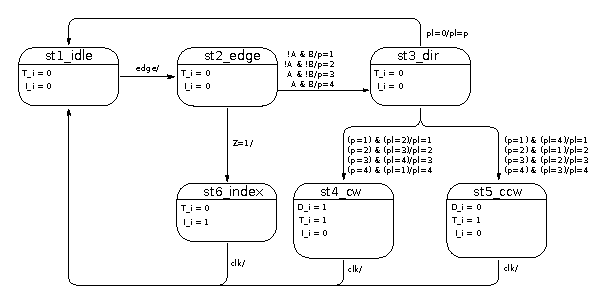
\includegraphics[width=.85\linewidth]{graphics/quad_state_machine}
	\caption[State machine of incremental quadrature decoder.]{State machine of the incremental quadrature decoder created for the MicroZed.}
	\label{fig:quadstatemachine}
\end{figure}
\paragraph{st1\_idle:} % (fold)
Is the initial state and the state that is returned to between edges on the quadrature signal.
Since the quadrature signal is not synchronous with the driving clock of the system the \texttt{rising\_edge()} and \texttt{falling\_edge()} functions cannot be used to determine edges.
Listing \ref{code:edge_detection} shows how an edge is detected on a signal. 
The current value of the signal is continuously compared to the last value, which is saved on every clock cycle.
If the two values are not equal an edge must have occured within the last clock cycle.
In this component both rising and falling edges are used and so any difference between the two is registered.
This code is repeated for all three input signals, with the exception that the \texttt{Z} channel sets \texttt{next\_state} to \texttt{st6\_index} instead.

\begin{listing}[H]
\begin{minted}{vhdl}
case (state) is
	when st1_idle =>
		if A_i /= last_A_i then
	        next_state <= st2_edge;
	    end if;
	    @$\vdots$@
\end{minted}
\caption{VHDL edge detection of asynchronous signal.}
\label{code:edge_detection}
\end{listing}

\paragraph{st2\_edge:} % (fold)
Is responsible for determining which phase is currently active.
The different phases can be seen in figure \ref{fig:quadrature}.
The phase is found simply by comparing the signals as seen in listing \ref{code:phase_detection}.
Regardless of the detected phase \texttt{next\_state} is set to \texttt{st3\_dir}.
\begin{listing}[H]
\begin{minted}{vhdl}
when st2_edge =>
	if A = '1' then
	    if B = '1' then
	        phase <= p4;
	    else
	        phase <= p3;
	    end if;
	    next_state <= st3_dir;
	    @$\vdots$@
\end{minted}
\caption{VHDL for phase detection in incremental quadrature.}
\label{code:phase_detection}
\end{listing}
\paragraph{st3\_dir:} % (fold)
Determines the current direction of travel.
This can be seen by comparing the current phase to the last phase.
Listing \ref{code:determine_direction} shows the structure of the code responsible for this step.
\begin{listing}[H]
\begin{minted}{vhdl}
when st3_dir =>
	if last_phase /= p0 then
	    if phase = p1 then
	        if last_phase = p4 then
	            next_state <= st5_ccw;
	        end if;
	        if last_phase = p2 then
	            next_state <= st4_cw;
	        end if;
	        next_last_phase <= p1;
	    end if;
	    if phase = p2 then
	    @$\vdots$@
    else
        next_last_phase <= phase;
        next_state <= st1_idle;
    end if;
\end{minted}
\caption[VHDL for determining direction of movement.]{VHDL for determining direction of movement in incremental quadrature.}
\label{code:determine_direction}
\end{listing}
As can be seen in the code there is a reference to phase 0.
This is required since the initial phase is unknown.
During the first run the direction-determination is skipped and \texttt{last\_phase} is initialized to \texttt{phase}.
On every subsequent run, depending on the direction, \texttt{next\_state} is set to either \texttt{st4\_cw} or \texttt{st5\_ccw}.
\paragraph{st4\_cw and st5\_ccw:} % (fold)
The SM is in these states for one clock cycle to allow for the outputs to be adjusted and a tick to be generated.
\paragraph{st6\_index:} % (fold)
The SM is in this state for one clock cycle when the \texttt{Z} input goes high and generates a signal to indicate that the index has been reached.
While this feature is unused in the cart position counter as it currently exists, it was decided to include it to allow future developers to use it if the need arises.

\paragraph{Cart Position Counter}~\\ % (fold)
\label{par:cart_position_counter}
This component maintains a counter which is incremented or decremented at every tick generated by the incremental quadrature decoder depending on the state of the direction signal.
If the endstop 1 signal is set high the counter is set to zero.
Upon booting the system the cart should be moved to the rightmost end-stop in order to calibrate the system.
Moving the cart will now increment the position with leftward motion and decrement with rightward motion.

\begin{figure}[h]
	\centering
	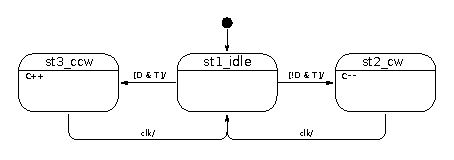
\includegraphics[width=.75\linewidth]{graphics/count_state_machine}
	\caption[State machine of the cart position counter]{State machine of the cart position counter created for the MicroZed.}
	\label{fig:countstatemachine}
\end{figure}

The SM of the system can be seen in figure \ref{fig:countstatemachine}.
In this figure \texttt{C} is \texttt{counter\_i}, \texttt{D} is \texttt{direction} and \texttt{T} is \texttt{tick}.
It should be noted that the end signal is treated as a reset signal and as such is not part of the actual SM.
Since it is essentially a reset signal handling of it is placed in the \texttt{sync process} to avoid an asynchronous reset of the values.
The code in question can be seen in listing \ref{code:cart_sync_proc}.

\begin{listing}[H]
\begin{minted}{vhdl}
SYNC_PROC:  process(clk)
	begin
	    if rising_edge(clk) then
	        if emend = '0' then
	            counter_i <= (others => '0');
	            state <= st1_idle;
	            cal_i <= '1';
	        else
	            state <= next_state;
	            counter_i <= next_counter_i;
	            last_T_i <= T_i;
	        end if;
	    end if;
	end process;
\end{minted}
\caption{Synchronous reset based on endstop signals.}
\label{code:cart_sync_proc}
\end{listing}

The SM has only three simple states.
\texttt{st1\_idle} which is the state where the SM waits for a rising edge on the tick signal, \texttt{T}.
If the direction signal, \texttt{D} is low when a tick arrives the SM proceeds to \texttt{st2\_cw} if the opposite is true it proceeds to \texttt{st3\_ccw}.
In those states the position variable, \texttt{counter\_i} is either decremented or incremented.

\paragraph{Test Benches}~\\ % (fold)
\label{par:test_benches}
A part of developing these components has been to develop and use test benches to verify code as it is being written.
VHDL was originally thought as a language to describe and simulate hardware and logic and has later been used as the programming language used to create FPGA designs.
All of the original features of the language are still present and as such it is possible to create a component which fully exercises whichever component is under development, the unit-under-test or UUT.
\\~\\
The test bench written for the cart position counter is comprised of three processes, the \texttt{clk\_proc} which is responsible for generating the driving clock for the component, \texttt{quad\_proce\_ccw} or \texttt{quad\_proce\_cw} for simulating the quadrature signal in either the counter-clockwise or the clockwise direction and finally the \texttt{stim\_proc} which is responsible for exercising any of the input signals.
\\~\\
\thomas{insert code snippet from testbench}

The UUT is instantiated as a component in the test bench and Vivado provides tools for investigating the flow of execution.
An excerpt illustrating the functionality can be seen in figure \ref{fig:testbench}.
As can be seen \texttt{B\_i} is leading \texttt{A\_i}, resulting in \texttt{D\_i} going \texttt{high}.
Since \texttt{emend\_i} is \texttt{high} the component starts counting on every rising edge of \texttt{T\_i}.
When \texttt{emend\_i} goes \texttt{low} the counter is reset and future ticks are ignored until \texttt{emend\_i} returns to \texttt{high}.

\begin{figure}[h]
	\centering
	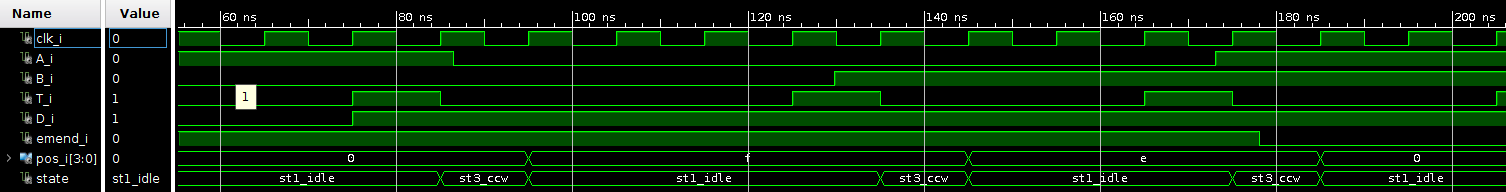
\includegraphics[width=\linewidth]{graphics/test_bench_narrow}
	\caption{Excerpt of testbench simulation results.}
	\label{fig:testbench}
\end{figure}

\paragraph{Packaging an AXI-Enabled IP Core}~\\ % (fold)
\label{par:ip_cores}
Once the component is confirmed functioning as intended, the component is packaged as an IP core capable of AXI communication.
Vivado provides an IP packager which auto-generates the files required for instantiating the components for AXI-communication.
The user can choose the number and width of the registers to be available in the instantiated AXI component.
In the generated files the user is expected to add their own code and alter existing code such that it correctly implements the desired functionality.
\\~\\
In relation to the components created in this project, the \texttt{.vhd} code files are imported to the project and the component instantiated.
Every user-defined port is brought out through the AXI component so that they can be constrained correctly in the \texttt{.xdc} constraint file.
Since every component is made as an IP core the system can be created using a block design.
For illustration purposes the block design of the full system has been included in figure \ref{fig:blockdesign}.
The rightmost blocks include three of the authors' designs and a Xilinx \texttt{axi\_gpio} block.
The GPIO block is used to handle hardware signals for creating a safety condition, enabling the motor driver and similar tasks.
\thomas{rewrite for proper safety condition}
As can be seen, a simple RGB LED controller has been written to handle the debug LEDs on the board.
By creating the component to control just a single LED, that code can be instantiated as many times as is required by the application and in any application.
In common for all of these blocks is that they require at least some of their input from the AXI bus.

\begin{figure}[h]
	\centering
	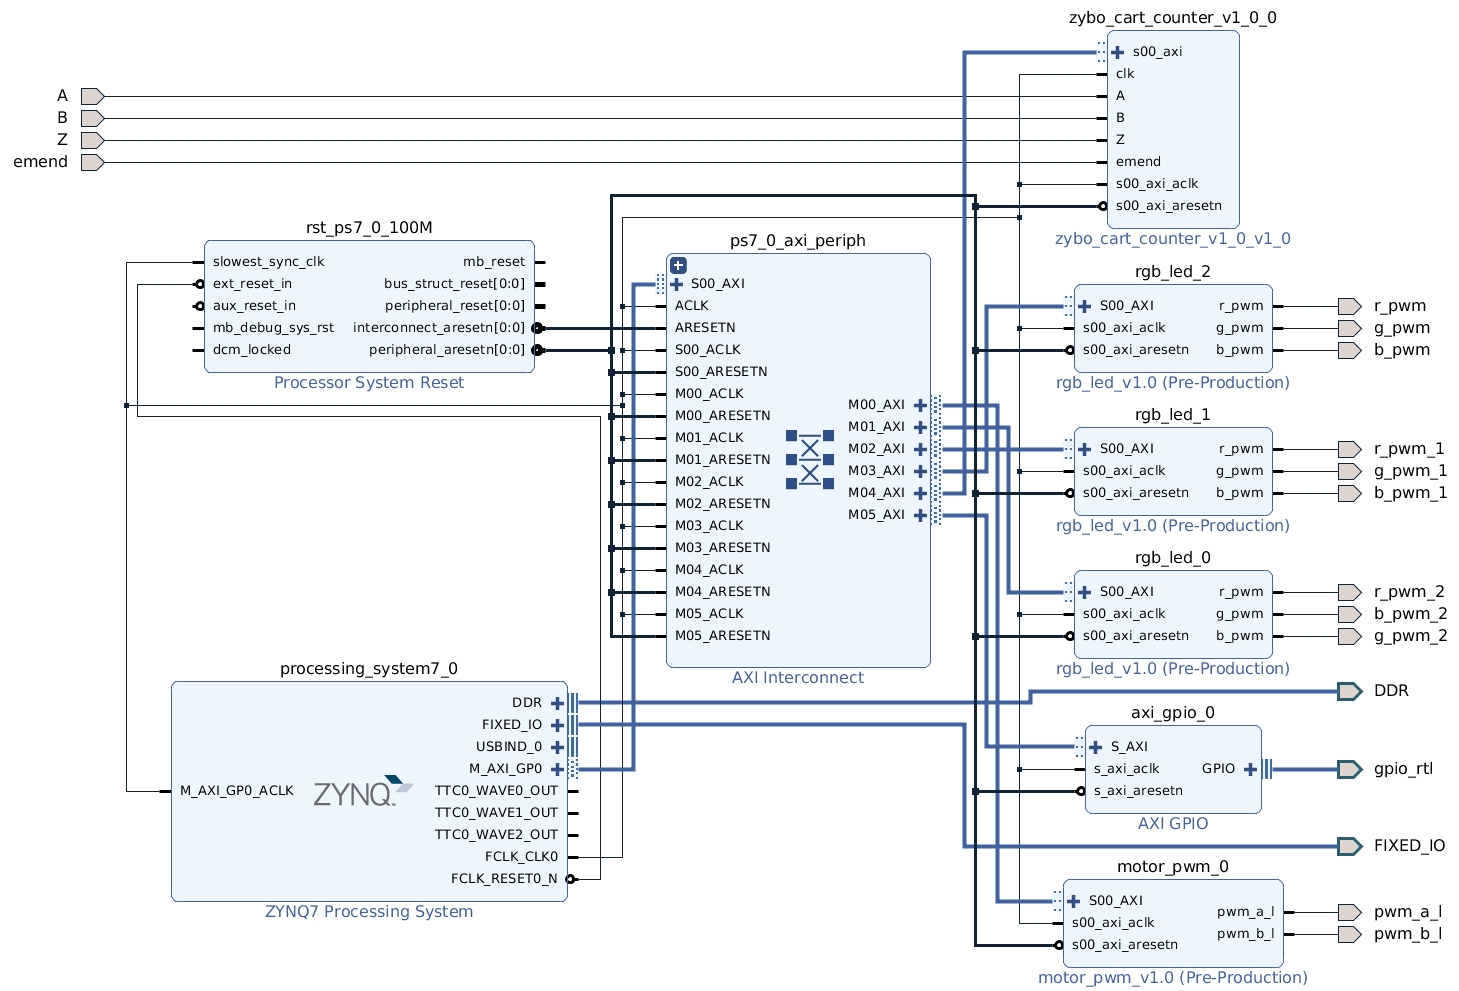
\includegraphics[width=\linewidth]{graphics/block_design}
	\caption{Vivado block design of the complete system.}
	\label{fig:blockdesign}
\end{figure}

\paragraph{Communication Through the AXI Bus}~\\ % (fold)
\label{par:communication_through_the_axi_bus}
In this project the AXI bus is used to communicate between PS and PL.
Doing this requires setup in both domains.
In PL registers are generated which the user can input data to.
An example of how this is set up can be seen in listing \ref{code:axiconnection}.
Individual bits in a register can be set to different variables and the remaining bits left unchanged.

\begin{listing}[H]
\begin{minted}{vhdl}
cart_counter_inst : cart_counter
	port map(
	    clk => clk,
	    A => A,
	    B => B,
	    Z => Z,
	    emend => emend,
	    cal => slv_reg0(1),
	    dir => slv_reg0(0),
	    pos => slv_reg1
	);
\end{minted}
\caption[Code showing the connection of AXI registers]{Code showing the connection of AXI registers to the cart position counter signals.}
\label{code:axiconnection}
\end{listing}

In PS these registers can be accessed using the \texttt{Xil\_In32()} and \texttt{Xil\_Out32()}.
These functions require an address and in the case of the output function, a payload to write to the register.
Each device in the design is given a base address which can be found in the \texttt{xparameters.h} header file which is generated for each hardware design.
Accessing a parameter is then done by adding the appropriate offset.
The offset is determined by the width of the registers.
In this case registers are 32 bits wide and so every offset is \texttt{0x04} bytes.
In code this is handled as seen in listing \ref{code:axiconnectionps}

\begin{listing}[H]
\begin{minted}{c}
#define CART_BASEADDR XPAR_ZYBO_CART_COUNTER_V1_0_0_BASEADDR

#define CAL_ADDR    0x00
#define DIR_ADDR    0x00
#define POS_ADDR    0x04
	
#define CALIBRATED  0x01
		@$\vdots$@
	
void get_position(uint32_t *position)
{
	if(is_calibrated() == CALIBRATED)
		*position = Xil_In32(CART_BASEADDR+POS_ADDR);
	else
		position = NULL;
}

		@$\vdots$@
void cart_task(void)
{
	uint32_t* pos = NULL;
	if(get_position(pos) != NULL)
	{
		//Do Something
	}
		@$\vdots$@
}
\end{minted}
\caption[Code handling communication with the cart position counter.]{Excerpt from the code written to handle the communication with the cart position counter. \texttt{is\_calibrated()} returns the status of calibration.}
\label{code:axiconnectionps}
\end{listing}

Here a wrapper function for \texttt{Xil\_In32()} is shown.
A number of these are written to simplify the code and reduce the risk of errors.
In this case the position is only valid if the calibration bit is set \texttt{high}.
When it is not, a null pointer is returned.
Rather than checking both the calibration status and the position, both can be done using a single function call.

\subsubsection{Interfacing the nRF24L01} % (fold)
\label{ssubs:nrf24l01}
~\\
The \texttt{nRFM} is interfaced through a standard SPI connection and a \texttt{CE} pin that is used to activate the chip. 
It also has an interrupt pin, but it was chosen not to use it and instead poll the device. 
Configuration of the device is done through SPI.

\paragraph{Setup} % (fold)
\label{par:nrfsetup}
~\\
The \texttt{nRFM} has multiple different modes of operations and care should be taken when setting it up.
The flowchart of figure \ref{fig:nrf_setup} gives an overview of what registers are set in order to gain the settings used in this project.
A description of each step and register is given below.
\begin{figure}[h]
	\centering
	\includegraphics[width=.8\linewidth]{graphics/nfr_setup}
	\caption{Flowchart showing the setup process of the \texttt{nRFM} module.}
	\label{fig:nrf_setup}
\end{figure}
\begin{itemize}
	\item \texttt{RF\_SETUP} register is set in order to gain 1Mbps air transmission and maximum output power in TX mode.
	\item \texttt{RF\_CH} register is used to set the channel used. It should be set differently for each \texttt{nRFM} pair.
	\item \texttt{SETUP\_AW} register is set to use the shortest available address width of three bytes.
	\item \texttt{EN\_AA} register is set to disable auto acknowledgement.
	\item \texttt{SETUP\_RETR} register is set to disable automatic retransmission.
\end{itemize}

The \texttt{PWR\_UP} bit is then set to \texttt{1} to power up the module. 
A wait of 4.5ms is then initiated to allow for proper start-up of the crystal.
\\~\\
If receive mode, \texttt{RX}, is needed the \texttt{PRIM\_RX} bit should be set to \texttt{1} and the receive address written to \texttt{RX\_ADDR\_P0}.
Furthermore \texttt{RX\_PW\_P0} is set to 2 in order to set the payload size to two bytes.
Finally \texttt{EN\_RX\_ADDR} is set to enable data on data pipe 0 and \texttt{CE} is set \texttt{high} to initiate the transition to \texttt{RX} mode.
\\~\\
If transmit mode, \texttt{TX}, is needed \texttt{PRIM\_RX} should be set to \texttt{0} and the transmit address should be written to \texttt{PRIM\_RX}.
Hereafter \texttt{CE} is set \texttt{high} to initiate the transition to \texttt{TX} mode.

\paragraph{Writing to a Register} % (fold)
\label{par:writing_to_a_register}
~\\
Figure \ref{fig:rw_register} illustrates the bits that are sent to the \texttt{nRFM} in order to write a value to a register. 
The three command bits specify if the action to be done is read or write.
The five address bits specify address of the register that is to be written to. 
The next one to five bytes is the value that are to be written to the register.

\begin{figure}[!h]
	\centering
	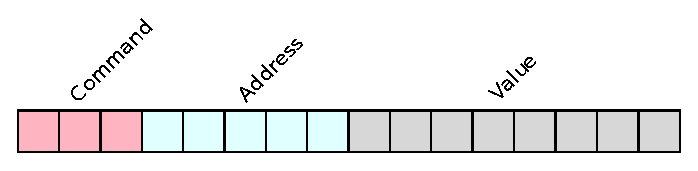
\includegraphics[width=.5\linewidth]{graphics/rw_register.eps}
	\caption[Writing bits to a register on nRF24L01.]{Bits written to the \texttt{nRFM} in order to write a value to a register. \texttt{Command} specifies if it is a read or write action, \texttt{Address} specifies the register address and \texttt{Value} specifies the value written to or read from the register.}
	\label{fig:rw_register}
\end{figure}
\thomas{fix figure to include arbitrary length value}

The C code in listing \ref{code:rf_write_register_code} is used to write a value to a register. 
Line 5 makes sure that a valid address and command is sent, regardless of the inputs.
Line 6 collects all bits that needs to be sent in one variable. 
The 2 bytes are sent using SPI in line 7, where it can also be seen that the answer from the \texttt{nRFM} is ignored as the null pointer is given as the input buffer.  

\begin{listing}[!h]
\begin{minted}{c}
#define W_REGISTER      0b00100000
#define REGISTER_MASK   0b00011111

void RF_write_register(XSpiPs *SPI_inst, u8 reg, u8 value){
	u8 cmd_addr =  (W_REGISTER | ( REGISTER_MASK & reg));
	u8 output_buffer[] = {cmd_addr, value};
	XSpiPs_PolledTransfer(SPI_inst, output_buffer, NULL, 2);
}
\end{minted}
\caption[C function that writes a value to a register on the nRFM]{Implementation of a C function that writes a register value to a specific register on the \texttt{nRFM}. Macros are shown for clarity.}
\label{code:rf_write_register_code}
\end{listing}

The corresponding SPI signals are measured and plotted in figure \ref{fig:nrf24_spi}.
It can be seen that the \texttt{MOSI} signal corresponds to \texttt{0b00100000, 0b00110101}, which means that the value \texttt{0b00110101} is written to the \texttt{RF\_CONFIG} register which has address \texttt{0x00}.
It can also be noted that data is available on the \texttt{MISO} signal. 
The \texttt{nRFM} always responds with the value of the \texttt{STATUS} when detecting a falling edge on \texttt{SS}.

\begin{figure}[h]
	\centering
    %% This file was created by matlab2tikz.
%
%The latest updates can be retrieved from
%  http://www.mathworks.com/matlabcentral/fileexchange/22022-matlab2tikz-matlab2tikz
%where you can also make suggestions and rate matlab2tikz.
%
\definecolor{mycolor1}{rgb}{0.00000,0.44700,0.74100}%
\definecolor{mycolor2}{rgb}{0.85000,0.32500,0.09800}%
\definecolor{mycolor3}{rgb}{0.92900,0.69400,0.12500}%
\definecolor{mycolor4}{rgb}{0.49400,0.18400,0.55600}%
%
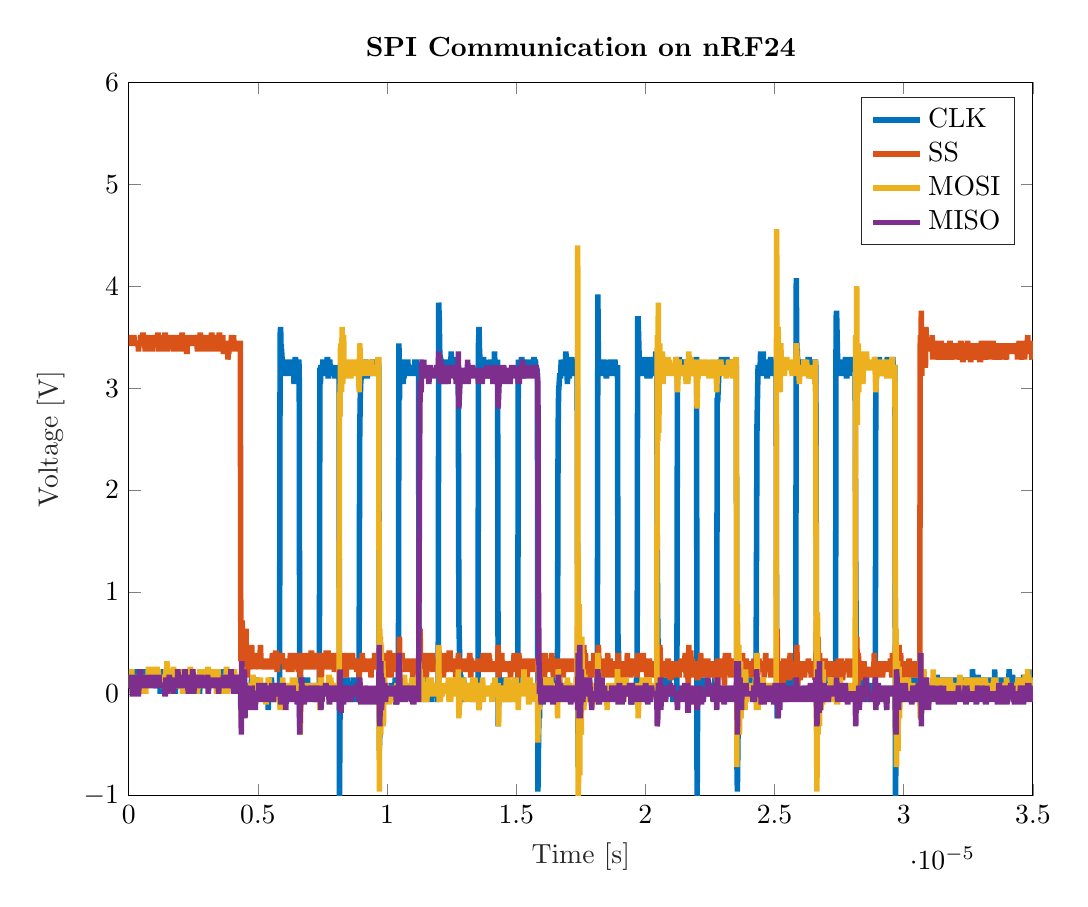
\begin{tikzpicture}

\begin{axis}[%
width=4.521in,
height=3.566in,
at={(0.758in,0.481in)},
scale only axis,
xmin=0,
xmax=3.5e-05,
xlabel style={font=\color{white!15!black}},
xlabel={Time [s]},
ymin=-1,
ymax=6,
ylabel style={font=\color{white!15!black}},
ylabel={Voltage [V]},
axis background/.style={fill=white},
title style={font=\bfseries},
title={SPI Communication on nRF24},
legend style={legend cell align=left, align=left, draw=white!15!black}
]
\addplot [color=mycolor1, line width=2.0pt]
  table[row sep=crcr]{%
-1.99999998784506e-08	0.0800000000000001\\
0	0.16\\
1.99999998784506e-08	0.16\\
3.99999997569012e-08	0.24\\
5.99999996353517e-08	0.0800000000000001\\
8.00000004019807e-08	0.0800000000000001\\
1.00000000280431e-07	0.16\\
1.20000000158882e-07	0.0800000000000001\\
1.40000000037332e-07	0.16\\
1.59999999915783e-07	0.16\\
1.79999999794234e-07	0.0800000000000001\\
1.99999999672684e-07	0.16\\
2.20000000439313e-07	0.16\\
2.40000000317764e-07	0.24\\
2.60000000196214e-07	0.0800000000000001\\
2.80000000074665e-07	0.0800000000000001\\
3.19999999831566e-07	0.24\\
3.39999999710017e-07	0.16\\
3.59999999588467e-07	0.16\\
3.80000000355096e-07	0.0800000000000001\\
4.20000000111997e-07	0.24\\
4.59999999868899e-07	0.0800000000000001\\
4.79999999747349e-07	0.16\\
4.999999996258e-07	0.0800000000000001\\
5.20000000392429e-07	0.24\\
5.40000000270879e-07	0.16\\
5.6000000014933e-07	0.24\\
5.80000000027781e-07	0.16\\
6.39999999663132e-07	0.16\\
6.60000000429761e-07	0.0800000000000001\\
6.80000000308212e-07	0.16\\
7.99999999578915e-07	0.16\\
8.20000000345544e-07	0.0800000000000001\\
8.40000000223995e-07	0.16\\
9.39999999616248e-07	0.16\\
9.60000000382877e-07	0.0800000000000001\\
9.80000000261327e-07	0.16\\
1.00000000013978e-06	0.16\\
1.02000000001823e-06	0.24\\
1.03999999989668e-06	0.0800000000000001\\
1.05999999977513e-06	0.0800000000000001\\
1.07999999965358e-06	0.24\\
1.10000000042021e-06	0.16\\
1.12000000029866e-06	0.16\\
1.14000000017711e-06	0.0800000000000001\\
1.17999999993401e-06	0.24\\
1.19999999981246e-06	0.16\\
1.21999999969091e-06	0\\
1.23999999956936e-06	0.0800000000000001\\
1.26000000033599e-06	0.24\\
1.28000000021444e-06	0\\
1.30000000009289e-06	0.16\\
1.31999999997134e-06	0.0800000000000001\\
1.35999999972825e-06	0.24\\
1.3799999996067e-06	0.16\\
1.40000000037332e-06	0.16\\
1.42000000025178e-06	0.0800000000000001\\
1.44000000013023e-06	0.0800000000000001\\
1.46000000000868e-06	0.16\\
1.51999999964403e-06	0.16\\
1.54000000041066e-06	0.0800000000000001\\
1.56000000028911e-06	0.24\\
1.58000000016756e-06	0.16\\
1.60000000004601e-06	0.16\\
1.61999999992446e-06	0.24\\
1.65999999968136e-06	0.0800000000000001\\
1.67999999955981e-06	0.16\\
1.72000000020489e-06	0.16\\
1.74000000008334e-06	0.0800000000000001\\
1.75999999996179e-06	0.16\\
1.79999999971869e-06	0\\
1.81999999959714e-06	0.0800000000000001\\
1.84000000036377e-06	0.24\\
1.86000000024222e-06	0.16\\
1.88000000012067e-06	0.16\\
1.89999999999912e-06	0.0800000000000001\\
1.91999999987758e-06	0.16\\
1.93999999975603e-06	0.0800000000000001\\
1.95999999963448e-06	0.16\\
1.98000000040111e-06	0.0800000000000001\\
2.00000000027956e-06	0.16\\
2.02000000015801e-06	0.16\\
2.04000000003646e-06	0.0800000000000001\\
2.14000000031689e-06	0.0800000000000001\\
2.18000000007379e-06	0.24\\
2.19999999995224e-06	0.0800000000000001\\
2.21999999983069e-06	0.16\\
2.23999999970914e-06	0.0800000000000001\\
2.28000000035422e-06	0.0800000000000001\\
2.30000000023267e-06	0.16\\
2.32000000011112e-06	0.16\\
2.33999999998957e-06	0.0800000000000001\\
2.35999999986802e-06	0.0800000000000001\\
2.37999999974647e-06	0.16\\
2.46000000014845e-06	0.16\\
2.48000000002691e-06	0.0800000000000001\\
2.49999999990536e-06	0.16\\
2.53999999966226e-06	0.16\\
2.56000000042889e-06	0\\
2.58000000030734e-06	0.16\\
2.60000000018579e-06	0.16\\
2.62000000006424e-06	0.0800000000000001\\
2.63999999994269e-06	0.0800000000000001\\
2.65999999982114e-06	0.16\\
2.67999999969959e-06	0.16\\
2.69999999957804e-06	0.0800000000000001\\
2.72000000034467e-06	0.0800000000000001\\
2.74000000022312e-06	0\\
2.76000000010157e-06	0.0800000000000001\\
2.77999999998002e-06	0.24\\
2.79999999985847e-06	0.0800000000000001\\
2.81999999973692e-06	0.16\\
2.83999999961537e-06	0.0800000000000001\\
2.860000000382e-06	0.16\\
2.92000000001735e-06	0.16\\
2.9399999998958e-06	0.0800000000000001\\
2.95999999977425e-06	0.24\\
2.9799999996527e-06	0.16\\
3.02000000029778e-06	0.16\\
3.04000000017624e-06	0.0800000000000001\\
3.06000000005469e-06	0.0800000000000001\\
3.07999999993314e-06	0.16\\
3.11999999969004e-06	0.16\\
3.13999999956849e-06	0.0800000000000001\\
3.16000000033512e-06	0.24\\
3.18000000021357e-06	0.16\\
3.20000000009202e-06	0.16\\
3.21999999997047e-06	0.24\\
3.23999999984892e-06	0.16\\
3.27999999960582e-06	0.16\\
3.30000000037245e-06	0.24\\
3.3200000002509e-06	0.0800000000000001\\
3.34000000012935e-06	0.24\\
3.3600000000078e-06	0.16\\
3.37999999988625e-06	0.16\\
3.3999999997647e-06	0.0800000000000001\\
3.41999999964315e-06	0.0800000000000001\\
3.44000000040978e-06	0.16\\
3.50000000004513e-06	0.16\\
3.51999999992358e-06	0.0800000000000001\\
3.53999999980203e-06	0.24\\
3.55999999968049e-06	0.0800000000000001\\
3.57999999955894e-06	0.16\\
3.60000000032556e-06	0.0800000000000001\\
3.62000000020402e-06	0.0800000000000001\\
3.64000000008247e-06	0.16\\
3.65999999996092e-06	0.16\\
3.67999999983937e-06	0.0800000000000001\\
3.69999999971782e-06	0.0800000000000001\\
3.71999999959627e-06	0.24\\
3.7400000003629e-06	0.0800000000000001\\
3.76000000024135e-06	0.16\\
3.7800000001198e-06	0.16\\
3.79999999999825e-06	0.0800000000000001\\
3.8199999998767e-06	0.16\\
3.88000000040023e-06	0.16\\
3.90000000027868e-06	0.0800000000000001\\
3.92000000015713e-06	0.16\\
3.94000000003558e-06	0.16\\
3.95999999991403e-06	0.0800000000000001\\
3.97999999979248e-06	0.16\\
3.99999999967093e-06	0.16\\
4.02000000043756e-06	0.0800000000000001\\
4.04000000031601e-06	0.16\\
4.06000000019446e-06	0.0800000000000001\\
4.08000000007291e-06	0.0800000000000001\\
4.09999999995136e-06	0.16\\
4.11999999982982e-06	0.0800000000000001\\
4.15999999958672e-06	0.0800000000000001\\
4.18000000035335e-06	0.16\\
4.2000000002318e-06	0.16\\
4.22000000011025e-06	0.0800000000000001\\
4.2399999999887e-06	0.0800000000000001\\
4.25999999986715e-06	0.16\\
4.32000000039068e-06	0.16\\
4.34000000026913e-06	-0.16\\
4.38000000002603e-06	0\\
4.39999999990448e-06	0.16\\
4.41999999978293e-06	0\\
4.43999999966138e-06	0\\
4.46000000042801e-06	-0.0800000000000001\\
4.48000000030646e-06	0.0800000000000001\\
4.52000000006336e-06	0.0800000000000001\\
4.53999999994181e-06	-0.0800000000000001\\
4.55999999982026e-06	0.0800000000000001\\
4.57999999969871e-06	0\\
4.62000000034379e-06	0\\
4.64000000022224e-06	0.0800000000000001\\
4.67999999997915e-06	-0.0800000000000001\\
4.6999999998576e-06	-0.0800000000000001\\
4.76000000038113e-06	0.16\\
4.78000000025958e-06	0\\
4.80000000013803e-06	0.0800000000000001\\
4.82000000001648e-06	0\\
4.83999999989493e-06	0\\
4.85999999977338e-06	0.0800000000000001\\
4.90000000041846e-06	0.0800000000000001\\
4.92000000029691e-06	0\\
4.94000000017536e-06	0.16\\
4.96000000005381e-06	0.0800000000000001\\
4.97999999993226e-06	0.0800000000000001\\
4.99999999981071e-06	0\\
5.01999999968916e-06	0\\
5.03999999956761e-06	0.0800000000000001\\
5.08000000021269e-06	0.0800000000000001\\
5.10000000009114e-06	0\\
5.11999999996959e-06	0\\
5.13999999984804e-06	0.0800000000000001\\
5.15999999972649e-06	0.0800000000000001\\
5.17999999960495e-06	0\\
5.24000000012848e-06	0\\
5.26000000000693e-06	0.0800000000000001\\
5.27999999988538e-06	0.0800000000000001\\
5.29999999976383e-06	0\\
5.31999999964228e-06	0.0800000000000001\\
5.34000000040891e-06	0.0800000000000001\\
5.36000000028736e-06	0\\
5.38000000016581e-06	0\\
5.40000000004426e-06	-0.16\\
5.41999999992271e-06	0.0800000000000001\\
5.45999999967961e-06	0.0800000000000001\\
5.47999999955806e-06	0\\
5.50000000032469e-06	0\\
5.52000000020314e-06	0.16\\
5.54000000008159e-06	0.0800000000000001\\
5.57999999983849e-06	0.0800000000000001\\
5.59999999971694e-06	0\\
5.61999999959539e-06	0\\
5.64000000036202e-06	0.0800000000000001\\
5.66000000024047e-06	-0.0800000000000001\\
5.69999999999737e-06	0.0800000000000001\\
5.71999999987582e-06	0\\
5.73999999975427e-06	0\\
5.75999999963273e-06	-0.0800000000000001\\
5.80000000027781e-06	0.0800000000000001\\
5.84000000003471e-06	0.0800000000000001\\
5.85999999991316e-06	3.52\\
5.87999999979161e-06	3.6\\
5.89999999967006e-06	3.36\\
5.92000000043669e-06	3.36\\
5.96000000019359e-06	3.2\\
5.98000000007204e-06	3.2\\
5.99999999995049e-06	3.12\\
6.01999999982894e-06	3.2\\
6.08000000035247e-06	3.2\\
6.10000000023092e-06	3.12\\
6.13999999998782e-06	3.28\\
6.15999999986627e-06	3.12\\
6.17999999974472e-06	3.2\\
6.19999999962317e-06	3.12\\
6.24000000026825e-06	3.28\\
6.2600000001467e-06	3.2\\
6.33999999966051e-06	3.2\\
6.36000000042714e-06	3.28\\
6.38000000030559e-06	3.2\\
6.40000000018404e-06	3.04\\
6.43999999994094e-06	3.28\\
6.45999999981939e-06	3.28\\
6.47999999969784e-06	3.2\\
6.49999999957629e-06	3.28\\
6.52000000034292e-06	3.2\\
6.54000000022137e-06	3.28\\
6.56000000009982e-06	3.2\\
6.57999999997827e-06	3.28\\
6.59999999985672e-06	3.2\\
6.61999999973517e-06	-0.32\\
6.63999999961362e-06	0.4\\
6.66000000038025e-06	-0.0800000000000001\\
6.6800000002587e-06	0.0800000000000001\\
6.7200000000156e-06	0.0800000000000001\\
6.73999999989405e-06	0.16\\
6.7599999997725e-06	0\\
6.77999999965095e-06	0.0800000000000001\\
6.80000000041758e-06	0\\
6.82000000029603e-06	0\\
6.84000000017448e-06	0.0800000000000001\\
6.86000000005293e-06	0\\
6.87999999993139e-06	0.0800000000000001\\
6.89999999980984e-06	0\\
6.91999999968829e-06	0.16\\
6.93999999956674e-06	0\\
6.96000000033337e-06	0.0800000000000001\\
6.98000000021182e-06	0\\
7.00000000009027e-06	0.0800000000000001\\
7.03999999984717e-06	0.0800000000000001\\
7.05999999972562e-06	0\\
7.1000000003707e-06	0\\
7.12000000024915e-06	0.0800000000000001\\
7.1400000001276e-06	0\\
7.16000000000605e-06	0\\
7.1799999998845e-06	0.0800000000000001\\
7.19999999976295e-06	0.0800000000000001\\
7.2199999996414e-06	-0.0800000000000001\\
7.24000000040803e-06	0\\
7.26000000028648e-06	0\\
7.28000000016493e-06	-0.0800000000000001\\
7.30000000004338e-06	0.0800000000000001\\
7.31999999992183e-06	0\\
7.35999999967873e-06	0\\
7.37999999955719e-06	0.0800000000000001\\
7.40000000032381e-06	3.2\\
7.42000000020226e-06	3.04\\
7.44000000008072e-06	3.2\\
7.45999999995917e-06	3.2\\
7.47999999983762e-06	3.12\\
7.51999999959452e-06	3.28\\
7.5600000002396e-06	3.12\\
7.58000000011805e-06	3.2\\
7.61999999987495e-06	3.2\\
7.6399999997534e-06	3.28\\
7.65999999963185e-06	3.2\\
7.68000000039848e-06	3.28\\
7.70000000027693e-06	3.28\\
7.72000000015538e-06	3.12\\
7.74000000003383e-06	3.12\\
7.77999999979073e-06	3.28\\
7.82000000043581e-06	3.12\\
7.84000000031426e-06	3.2\\
7.89999999994961e-06	3.2\\
7.91999999982806e-06	3.12\\
7.93999999970652e-06	3.2\\
7.95999999958497e-06	3.2\\
7.98000000035159e-06	3.12\\
8.00000000023005e-06	3.12\\
8.0200000001085e-06	3.2\\
8.14000000026738e-06	3.2\\
8.16000000014583e-06	-1.04\\
8.18000000002428e-06	-0.16\\
8.19999999990273e-06	-0.0800000000000001\\
8.21999999978118e-06	-0.16\\
8.26000000042626e-06	0.0800000000000001\\
8.28000000030471e-06	0.0800000000000001\\
8.30000000018316e-06	0\\
8.32000000006161e-06	0\\
8.33999999994006e-06	0.16\\
8.37999999969696e-06	-0.0800000000000001\\
8.39999999957541e-06	0\\
8.42000000034204e-06	0\\
8.44000000022049e-06	0.0800000000000001\\
8.46000000009894e-06	0\\
8.47999999997739e-06	0.16\\
8.49999999985585e-06	-0.0800000000000001\\
8.5199999997343e-06	0.0800000000000001\\
8.53999999961275e-06	0\\
8.56000000037938e-06	0\\
8.58000000025783e-06	0.0800000000000001\\
8.60000000013628e-06	0\\
8.62000000001473e-06	0.0800000000000001\\
8.63999999989318e-06	-0.0800000000000001\\
8.65999999977163e-06	0\\
8.67999999965008e-06	0\\
8.72000000029516e-06	0.16\\
8.74000000017361e-06	0\\
8.76000000005206e-06	0.0800000000000001\\
8.77999999993051e-06	0\\
8.81999999968741e-06	0\\
8.83999999956586e-06	-0.0800000000000001\\
8.86000000033249e-06	0.0800000000000001\\
8.88000000021094e-06	0\\
8.90000000008939e-06	0.0800000000000001\\
8.91999999996784e-06	0.4\\
8.93999999984629e-06	2.48\\
8.95999999972474e-06	2.88\\
8.97999999960319e-06	3.04\\
9.00000000036982e-06	3.12\\
9.07999999988363e-06	3.12\\
9.09999999976208e-06	3.28\\
9.11999999964053e-06	3.12\\
9.16000000028561e-06	3.28\\
9.18000000016406e-06	3.2\\
9.20000000004251e-06	3.2\\
9.21999999992096e-06	3.12\\
9.23999999979941e-06	3.12\\
9.25999999967786e-06	3.2\\
9.34000000007984e-06	3.2\\
9.35999999995829e-06	3.12\\
9.37999999983674e-06	3.2\\
9.41999999959364e-06	3.2\\
9.44000000036027e-06	3.28\\
9.46000000023872e-06	3.2\\
9.48000000011717e-06	3.28\\
9.49999999999562e-06	3.2\\
9.51999999987407e-06	3.2\\
9.53999999975252e-06	3.12\\
9.55999999963097e-06	3.2\\
9.60000000027605e-06	3.2\\
9.6200000001545e-06	3.12\\
9.65999999991141e-06	3.28\\
9.67999999978986e-06	3.2\\
9.69999999966831e-06	-0.56\\
9.74000000031339e-06	-0.24\\
9.76000000019184e-06	0\\
9.81999999982719e-06	0\\
9.83999999970564e-06	0.0800000000000001\\
9.85999999958409e-06	0\\
9.90000000022917e-06	0\\
9.92000000010762e-06	0.0800000000000001\\
9.93999999998607e-06	0.0800000000000001\\
9.95999999986452e-06	0\\
9.97999999974297e-06	0\\
9.99999999962142e-06	0.0800000000000001\\
1.00200000003881e-05	0\\
1.00400000002665e-05	0.0800000000000001\\
1.0060000000145e-05	0\\
1.00800000000234e-05	0.0800000000000001\\
1.00999999999019e-05	0\\
1.01199999997803e-05	0.0800000000000001\\
1.01399999996588e-05	0.0800000000000001\\
1.01600000004254e-05	0\\
1.02399999999392e-05	0\\
1.02599999998176e-05	-0.0800000000000001\\
1.03200000003412e-05	0.16\\
1.03400000002196e-05	-0.0800000000000001\\
1.03600000000981e-05	-0.0800000000000001\\
1.03799999999765e-05	0.0800000000000001\\
1.0399999999855e-05	0\\
1.04199999997334e-05	0.0800000000000001\\
1.04399999996119e-05	0.0800000000000001\\
1.04600000003785e-05	3.44\\
1.0480000000257e-05	2.88\\
1.05000000001354e-05	3.28\\
1.05200000000139e-05	3.2\\
1.05399999998923e-05	3.2\\
1.05599999997708e-05	3.12\\
1.06000000004158e-05	3.28\\
1.06200000002943e-05	3.04\\
1.06400000001727e-05	3.12\\
1.06600000000512e-05	3.12\\
1.06999999998081e-05	3.28\\
1.07199999996865e-05	3.2\\
1.07600000003316e-05	3.2\\
1.07800000002101e-05	3.12\\
1.08000000000885e-05	3.28\\
1.08399999998454e-05	3.12\\
1.08599999997239e-05	3.2\\
1.10199999996397e-05	3.2\\
1.10400000004063e-05	3.12\\
1.10800000001632e-05	3.28\\
1.11000000000416e-05	3.2\\
1.11199999999201e-05	3.2\\
1.11399999997985e-05	3.28\\
1.11800000004436e-05	3.12\\
1.12000000003221e-05	3.2\\
1.12200000002005e-05	3.12\\
1.1240000000079e-05	0\\
1.12599999999574e-05	0.32\\
1.12799999998359e-05	0.0800000000000001\\
1.12999999997143e-05	0.0800000000000001\\
1.13400000003594e-05	-0.0800000000000001\\
1.13600000002378e-05	0.0800000000000001\\
1.13800000001163e-05	0\\
1.13999999999947e-05	0\\
1.14199999998732e-05	0.0800000000000001\\
1.14599999996301e-05	0.0800000000000001\\
1.14800000003967e-05	0\\
1.15000000002752e-05	0.16\\
1.15400000000321e-05	-0.0800000000000001\\
1.1579999999789e-05	0.0800000000000001\\
1.15999999996674e-05	0\\
1.16200000004341e-05	0\\
1.16400000003125e-05	0.0800000000000001\\
1.1660000000191e-05	0\\
1.16800000000694e-05	0\\
1.16999999999479e-05	-0.0800000000000001\\
1.17399999997048e-05	0.0800000000000001\\
1.17800000003498e-05	0.0800000000000001\\
1.18000000002283e-05	0\\
1.18399999999852e-05	0\\
1.18599999998636e-05	0.0800000000000001\\
1.18799999997421e-05	0\\
1.18999999996205e-05	0.0800000000000001\\
1.19200000003872e-05	0.0800000000000001\\
1.19400000002656e-05	-0.0800000000000001\\
1.19800000000225e-05	0.0800000000000001\\
1.1999999999901e-05	3.84\\
1.20199999997794e-05	3.68\\
1.20399999996579e-05	3.36\\
1.20600000004245e-05	3.28\\
1.2080000000303e-05	3.28\\
1.21000000001814e-05	3.2\\
1.21200000000599e-05	3.2\\
1.21599999998168e-05	3.04\\
1.21799999996952e-05	3.28\\
1.21999999995737e-05	3.12\\
1.22200000003403e-05	3.2\\
1.22400000002187e-05	3.2\\
1.22600000000972e-05	3.04\\
1.22799999999756e-05	3.2\\
1.22999999998541e-05	3.28\\
1.23199999997325e-05	3.12\\
1.2339999999611e-05	3.12\\
1.23600000003776e-05	3.28\\
1.23800000002561e-05	3.12\\
1.24000000001345e-05	3.28\\
1.2420000000013e-05	3.2\\
1.24399999998914e-05	3.28\\
1.24599999997699e-05	3.12\\
1.24799999996483e-05	3.36\\
1.25400000001719e-05	3.12\\
1.25600000000503e-05	3.28\\
1.25799999999288e-05	3.2\\
1.26399999995641e-05	3.2\\
1.26600000003307e-05	3.28\\
1.26800000002092e-05	3.28\\
1.27000000000876e-05	3.2\\
1.27199999999661e-05	3.28\\
1.27399999998445e-05	3.2\\
1.2759999999723e-05	2.88\\
1.27799999996014e-05	0.72\\
1.28200000002465e-05	0.24\\
1.2840000000125e-05	0.16\\
1.28600000000034e-05	0.16\\
1.28799999998819e-05	0\\
1.28999999997603e-05	0.0800000000000001\\
1.29199999996388e-05	-0.0800000000000001\\
1.29400000004054e-05	0\\
1.29600000002839e-05	0.16\\
1.29800000001623e-05	0.0800000000000001\\
1.30000000000408e-05	0.0800000000000001\\
1.30199999999192e-05	0\\
1.30399999997977e-05	0\\
1.30599999996761e-05	0.0800000000000001\\
1.30800000004427e-05	0.0800000000000001\\
1.31000000003212e-05	0\\
1.31599999999565e-05	0\\
1.3179999999835e-05	0.0800000000000001\\
1.31999999997134e-05	0.0800000000000001\\
1.32199999995919e-05	0\\
1.32400000003585e-05	0.0800000000000001\\
1.3260000000237e-05	0\\
1.32999999999939e-05	0\\
1.33199999998723e-05	-0.0800000000000001\\
1.33399999997508e-05	0.0800000000000001\\
1.33800000003959e-05	0.0800000000000001\\
1.34000000002743e-05	0\\
1.34200000001528e-05	0\\
1.34400000000312e-05	0.0800000000000001\\
1.34599999999097e-05	0\\
1.35200000004332e-05	0\\
1.35400000003116e-05	3.44\\
1.35600000001901e-05	3.6\\
1.35800000000685e-05	3.36\\
1.3599999999947e-05	3.28\\
1.36199999998254e-05	3.28\\
1.36399999997039e-05	3.2\\
1.36599999995823e-05	3.2\\
1.3680000000349e-05	3.12\\
1.37000000002274e-05	3.28\\
1.37399999999843e-05	3.28\\
1.37799999997412e-05	3.12\\
1.37999999996197e-05	3.12\\
1.38200000003863e-05	3.2\\
1.38999999999001e-05	3.2\\
1.39199999997786e-05	3.12\\
1.3939999999657e-05	3.12\\
1.39600000004236e-05	3.28\\
1.39800000003021e-05	3.2\\
1.40399999999374e-05	3.2\\
1.40599999998159e-05	3.28\\
1.40799999996943e-05	3.2\\
1.41200000003394e-05	3.2\\
1.41400000002179e-05	3.12\\
1.41600000000963e-05	3.36\\
1.41799999999748e-05	3.2\\
1.41999999998532e-05	3.2\\
1.42199999997317e-05	3.12\\
1.42399999996101e-05	3.2\\
1.42600000003767e-05	3.2\\
1.42800000002552e-05	3.28\\
1.43000000001337e-05	-0.32\\
1.43200000000121e-05	0.4\\
1.43399999998906e-05	0.0800000000000001\\
1.44000000004141e-05	0.0800000000000001\\
1.44200000002925e-05	0.16\\
1.4440000000171e-05	0\\
1.44600000000494e-05	0.16\\
1.44799999999279e-05	0.0800000000000001\\
1.44999999998063e-05	0.0800000000000001\\
1.45199999996848e-05	-0.0800000000000001\\
1.45399999995632e-05	0.0800000000000001\\
1.45600000003299e-05	0.0800000000000001\\
1.45800000002083e-05	0\\
1.46000000000868e-05	0\\
1.46199999999652e-05	0.0800000000000001\\
1.46399999998437e-05	0.0800000000000001\\
1.46599999997221e-05	0.16\\
1.46799999996006e-05	0\\
1.47000000003672e-05	0.0800000000000001\\
1.47200000002456e-05	-0.0800000000000001\\
1.47600000000025e-05	0.0800000000000001\\
1.4779999999881e-05	0\\
1.47999999997595e-05	0.0800000000000001\\
1.48199999996379e-05	0\\
1.48400000004045e-05	0.0800000000000001\\
1.4860000000283e-05	0\\
1.48800000001614e-05	0.0800000000000001\\
1.49000000000399e-05	0.0800000000000001\\
1.49199999999183e-05	0\\
1.49399999997968e-05	0\\
1.49599999996752e-05	0.0800000000000001\\
1.49800000004419e-05	0.0800000000000001\\
1.50000000003203e-05	-0.0800000000000001\\
1.50200000001988e-05	0\\
1.50400000000772e-05	0.16\\
1.50599999999557e-05	0.0800000000000001\\
1.50799999998341e-05	3.28\\
1.50999999997126e-05	3.12\\
1.5119999999591e-05	3.2\\
1.51800000001145e-05	3.2\\
1.5199999999993e-05	3.28\\
1.52199999998714e-05	3.28\\
1.52599999996283e-05	3.12\\
1.5280000000395e-05	3.12\\
1.53000000002734e-05	3.2\\
1.53200000001519e-05	3.2\\
1.53400000000303e-05	3.12\\
1.53599999999088e-05	3.28\\
1.53799999997872e-05	3.2\\
1.54200000004323e-05	3.2\\
1.54400000003108e-05	3.12\\
1.54600000001892e-05	3.2\\
1.54800000000677e-05	3.2\\
1.54999999999461e-05	3.12\\
1.55199999998246e-05	3.2\\
1.5539999999703e-05	3.12\\
1.55800000003481e-05	3.28\\
1.56000000002265e-05	3.2\\
1.56599999998619e-05	3.2\\
1.56799999997403e-05	3.28\\
1.56999999996188e-05	3.28\\
1.57200000003854e-05	3.2\\
1.57400000002639e-05	3.28\\
1.57800000000208e-05	3.12\\
1.57999999998992e-05	3.2\\
1.58199999997777e-05	3.12\\
1.58399999996561e-05	-0.96\\
1.58800000003012e-05	-0.16\\
1.59000000001797e-05	-0.24\\
1.59200000000581e-05	0\\
1.59399999999366e-05	0.0800000000000001\\
1.5959999999815e-05	-0.0800000000000001\\
1.59799999996935e-05	0.0800000000000001\\
1.60200000003385e-05	-0.0800000000000001\\
1.6040000000217e-05	0\\
1.60600000000954e-05	0\\
1.60799999999739e-05	0.0800000000000001\\
1.60999999998523e-05	0\\
1.61199999997308e-05	0\\
1.61399999996092e-05	0.0800000000000001\\
1.61600000003759e-05	0.0800000000000001\\
1.61800000002543e-05	-0.0800000000000001\\
1.62000000001328e-05	0\\
1.62200000000112e-05	-0.0800000000000001\\
1.62599999997681e-05	0.16\\
1.63000000004132e-05	-0.0800000000000001\\
1.63200000002917e-05	0\\
1.63400000001701e-05	0\\
1.63600000000486e-05	0.16\\
1.6379999999927e-05	-0.0800000000000001\\
1.63999999998055e-05	0.0800000000000001\\
1.64199999996839e-05	-0.0800000000000001\\
1.64399999995624e-05	0.16\\
1.64800000002074e-05	0\\
1.65000000000859e-05	0\\
1.65199999999643e-05	0.0800000000000001\\
1.65399999998428e-05	0.0800000000000001\\
1.65599999997212e-05	-0.0800000000000001\\
1.65799999995997e-05	0\\
1.66000000003663e-05	0.48\\
1.66200000002448e-05	2.56\\
1.66400000001232e-05	2.96\\
1.66799999998801e-05	3.12\\
1.6719999999637e-05	3.12\\
1.67400000004037e-05	3.28\\
1.67600000002821e-05	3.12\\
1.67800000001606e-05	3.2\\
1.6800000000039e-05	3.12\\
1.68399999997959e-05	3.28\\
1.68599999996744e-05	3.2\\
1.69000000003194e-05	3.2\\
1.69200000001979e-05	3.36\\
1.69599999999548e-05	3.2\\
1.69799999998332e-05	3.04\\
1.69999999997117e-05	3.2\\
1.70199999995901e-05	3.2\\
1.70400000003568e-05	3.12\\
1.70600000002352e-05	3.12\\
1.70800000001137e-05	3.2\\
1.71199999998706e-05	3.2\\
1.7139999999749e-05	3.28\\
1.71599999996275e-05	3.28\\
1.71800000003941e-05	3.2\\
1.7220000000151e-05	3.2\\
1.72400000000295e-05	3.12\\
1.72599999999079e-05	3.2\\
1.72799999997864e-05	3.12\\
1.72999999996648e-05	3.28\\
1.73200000004314e-05	3.2\\
1.73400000003099e-05	3.28\\
1.73600000001883e-05	3.2\\
1.73800000000668e-05	0.0800000000000001\\
1.73999999999452e-05	-0.72\\
1.74199999998237e-05	0.16\\
1.74399999997021e-05	-0.0800000000000001\\
1.74599999995806e-05	-0.0800000000000001\\
1.74800000003472e-05	0.0800000000000001\\
1.75000000002257e-05	-0.0800000000000001\\
1.75200000001041e-05	0.0800000000000001\\
1.7559999999861e-05	-0.0800000000000001\\
1.75799999997395e-05	0.16\\
1.75999999996179e-05	0\\
1.76200000003846e-05	0.0800000000000001\\
1.7640000000263e-05	0.0800000000000001\\
1.76600000001415e-05	0\\
1.76800000000199e-05	0.16\\
1.77199999997768e-05	0\\
1.77800000003003e-05	0\\
1.78000000001788e-05	0.0800000000000001\\
1.78200000000572e-05	0\\
1.78399999999357e-05	0\\
1.78599999998141e-05	0.0800000000000001\\
1.78799999996926e-05	0\\
1.7899999999571e-05	0\\
1.79200000003377e-05	0.0800000000000001\\
1.79400000002161e-05	0\\
1.79600000000946e-05	0.0800000000000001\\
1.7979999999973e-05	0\\
1.79999999998515e-05	0.0800000000000001\\
1.80199999997299e-05	0\\
1.81000000001319e-05	0\\
1.81200000000104e-05	0.16\\
1.81399999998888e-05	0.0800000000000001\\
1.81599999997673e-05	3.92\\
1.81799999996457e-05	3.28\\
1.82000000004123e-05	3.2\\
1.82999999998046e-05	3.2\\
1.8319999999683e-05	3.12\\
1.83399999995615e-05	3.2\\
1.83600000003281e-05	3.2\\
1.83800000002066e-05	3.28\\
1.8400000000085e-05	3.2\\
1.84199999999635e-05	3.28\\
1.84399999998419e-05	3.12\\
1.84599999997204e-05	3.2\\
1.84799999995988e-05	3.12\\
1.85000000003654e-05	3.12\\
1.85200000002439e-05	3.28\\
1.85400000001223e-05	3.12\\
1.85600000000008e-05	3.2\\
1.85799999998792e-05	3.2\\
1.85999999997577e-05	3.12\\
1.86199999996361e-05	3.28\\
1.86400000004028e-05	3.2\\
1.86600000002812e-05	3.28\\
1.87000000000381e-05	3.12\\
1.87199999999166e-05	3.28\\
1.8739999999795e-05	3.12\\
1.87599999996735e-05	3.2\\
1.87800000004401e-05	3.12\\
1.8820000000197e-05	3.28\\
1.88599999999539e-05	3.12\\
1.88799999998324e-05	3.2\\
1.89199999995893e-05	3.2\\
1.89400000003559e-05	0.4\\
1.89600000002343e-05	0.4\\
1.89800000001128e-05	0.16\\
1.89999999999912e-05	0.16\\
1.90199999998697e-05	0\\
1.90399999997481e-05	0\\
1.90599999996266e-05	0.0800000000000001\\
1.90800000003932e-05	0\\
1.91000000002717e-05	0\\
1.91200000001501e-05	0.0800000000000001\\
1.91400000000286e-05	0\\
1.9159999999907e-05	0.0800000000000001\\
1.91999999996639e-05	0.0800000000000001\\
1.92200000004306e-05	0\\
1.92600000001875e-05	0\\
1.92800000000659e-05	0.0800000000000001\\
1.93199999998228e-05	0.0800000000000001\\
1.93399999997013e-05	0\\
1.93599999995797e-05	0\\
1.93800000003463e-05	0.0800000000000001\\
1.94200000001032e-05	0.0800000000000001\\
1.94599999998601e-05	-0.0800000000000001\\
1.94799999997386e-05	-0.0800000000000001\\
1.9499999999617e-05	0.0800000000000001\\
1.95200000003837e-05	0\\
1.95400000002621e-05	0\\
1.95600000001406e-05	0.0800000000000001\\
1.9580000000019e-05	0.0800000000000001\\
1.95999999998975e-05	0\\
1.96199999997759e-05	0\\
1.9660000000421e-05	0.16\\
1.96800000002995e-05	0.0800000000000001\\
1.97000000001779e-05	3.68\\
1.97200000000564e-05	3.68\\
1.97599999998133e-05	3.28\\
1.97799999996917e-05	3.12\\
1.98200000003368e-05	3.28\\
1.98600000000937e-05	3.12\\
1.98799999999721e-05	3.2\\
1.98999999998506e-05	3.12\\
1.9919999999729e-05	3.2\\
1.99399999996075e-05	3.2\\
1.99600000003741e-05	3.28\\
2.0000000000131e-05	3.28\\
2.00200000000095e-05	3.2\\
2.00399999998879e-05	3.2\\
2.00599999997664e-05	3.12\\
2.00799999996448e-05	3.12\\
2.01000000004115e-05	3.28\\
2.01200000002899e-05	3.2\\
2.01400000001684e-05	3.28\\
2.01600000000468e-05	3.12\\
2.01799999999253e-05	3.12\\
2.02199999996822e-05	3.28\\
2.02399999995606e-05	3.28\\
2.02600000003272e-05	3.2\\
2.02800000002057e-05	3.28\\
2.03000000000841e-05	3.12\\
2.03199999999626e-05	3.2\\
2.0339999999841e-05	3.2\\
2.03599999997195e-05	3.28\\
2.03799999995979e-05	3.2\\
2.04000000003646e-05	3.36\\
2.0420000000243e-05	3.2\\
2.04400000001215e-05	3.28\\
2.04599999999999e-05	1.36\\
2.04799999998784e-05	0.64\\
2.05199999996353e-05	0.0800000000000001\\
2.05600000002804e-05	0.0800000000000001\\
2.05800000001588e-05	0\\
2.06000000000373e-05	0.24\\
2.06199999999157e-05	0\\
2.06399999997942e-05	0.16\\
2.06599999996726e-05	0\\
2.07000000003177e-05	0.16\\
2.07200000001961e-05	0\\
2.0759999999953e-05	0\\
2.07799999998315e-05	0.0800000000000001\\
2.08199999995884e-05	0.0800000000000001\\
2.0840000000355e-05	0\\
2.08600000002335e-05	0.0800000000000001\\
2.08999999999904e-05	0.0800000000000001\\
2.09199999998688e-05	0.16\\
2.09399999997473e-05	0\\
2.09599999996257e-05	0\\
2.09800000003924e-05	0.0800000000000001\\
2.10000000002708e-05	0\\
2.10200000001493e-05	0\\
2.10400000000277e-05	0.0800000000000001\\
2.10599999999062e-05	-0.0800000000000001\\
2.10999999996631e-05	0.0800000000000001\\
2.11200000004297e-05	0\\
2.11400000003081e-05	0\\
2.11600000001866e-05	0.0800000000000001\\
2.11999999999435e-05	-0.0800000000000001\\
2.12199999998219e-05	0.0800000000000001\\
2.12399999997004e-05	3.28\\
2.12599999995788e-05	3.28\\
2.12800000003455e-05	3.2\\
2.13000000002239e-05	3.28\\
2.13200000001024e-05	3.28\\
2.13399999999808e-05	3.2\\
2.13799999997377e-05	3.2\\
2.13999999996162e-05	3.28\\
2.14200000003828e-05	3.2\\
2.14400000002613e-05	3.2\\
2.14600000001397e-05	3.28\\
2.14999999998966e-05	3.12\\
2.15399999996535e-05	3.28\\
2.15600000004201e-05	3.2\\
2.1600000000177e-05	3.2\\
2.16200000000555e-05	3.28\\
2.16399999999339e-05	3.2\\
2.16999999995693e-05	3.2\\
2.17200000003359e-05	3.12\\
2.17400000002144e-05	3.2\\
2.18199999997282e-05	3.2\\
2.18399999996066e-05	3.12\\
2.18800000002517e-05	3.28\\
2.19000000001301e-05	3.2\\
2.1939999999887e-05	3.2\\
2.19599999997655e-05	3.28\\
2.1979999999644e-05	3.28\\
2.20000000004106e-05	-1.2\\
2.2020000000289e-05	-0.16\\
2.20400000001675e-05	0\\
2.20600000000459e-05	-0.0800000000000001\\
2.20999999998028e-05	0.0800000000000001\\
2.21199999996813e-05	0\\
2.21600000003264e-05	0\\
2.22000000000833e-05	0.16\\
2.22199999999617e-05	0.0800000000000001\\
2.22399999998402e-05	0.0800000000000001\\
2.22599999997186e-05	0\\
2.22799999995971e-05	0\\
2.23000000003637e-05	0.0800000000000001\\
2.23200000002421e-05	0\\
2.23400000001206e-05	0.0800000000000001\\
2.2359999999999e-05	0\\
2.23799999998775e-05	0.0800000000000001\\
2.23999999997559e-05	0\\
2.2440000000401e-05	0\\
2.24600000002795e-05	0.0800000000000001\\
2.24800000001579e-05	0.0800000000000001\\
2.25000000000364e-05	0\\
2.25399999997933e-05	0\\
2.25599999996717e-05	0.0800000000000001\\
2.26400000000737e-05	0.0800000000000001\\
2.26599999999522e-05	0\\
2.26799999998306e-05	0.16\\
2.26999999997091e-05	0.0800000000000001\\
2.27199999995875e-05	0.0800000000000001\\
2.27400000003541e-05	0\\
2.27600000002326e-05	0.0800000000000001\\
2.2780000000111e-05	2.88\\
2.27999999999895e-05	2.88\\
2.28399999997464e-05	3.12\\
2.28599999996248e-05	3.2\\
2.28800000003915e-05	3.2\\
2.29000000002699e-05	3.28\\
2.29200000001484e-05	3.12\\
2.29400000000268e-05	3.28\\
2.29599999999053e-05	3.28\\
2.29799999997837e-05	3.2\\
2.29999999996622e-05	3.2\\
2.30200000004288e-05	3.28\\
2.30400000003073e-05	3.2\\
2.31199999998211e-05	3.2\\
2.31399999996995e-05	3.28\\
2.3159999999578e-05	3.28\\
2.31800000003446e-05	3.2\\
2.32399999999799e-05	3.2\\
2.32599999998584e-05	3.12\\
2.32999999996153e-05	3.28\\
2.33200000003819e-05	3.2\\
2.33800000000173e-05	3.2\\
2.33999999998957e-05	3.28\\
2.34199999997742e-05	3.12\\
2.34600000004193e-05	3.28\\
2.34800000002977e-05	3.2\\
2.35200000000546e-05	3.2\\
2.35399999999331e-05	-0.64\\
2.35599999998115e-05	-0.96\\
2.35999999995684e-05	-0.0800000000000001\\
2.3620000000335e-05	0\\
2.36400000002135e-05	0\\
2.36600000000919e-05	0.0800000000000001\\
2.36999999998488e-05	0.0800000000000001\\
2.37199999997273e-05	0\\
2.37399999996057e-05	0.0800000000000001\\
2.38000000001293e-05	0.0800000000000001\\
2.38200000000077e-05	0\\
2.38399999998862e-05	0\\
2.38599999997646e-05	0.0800000000000001\\
2.38799999996431e-05	0\\
2.39000000004097e-05	0.0800000000000001\\
2.39600000000451e-05	0.0800000000000001\\
2.39799999999235e-05	0\\
2.40399999995589e-05	0\\
2.40600000003255e-05	0.16\\
2.40800000002039e-05	0.0800000000000001\\
2.41199999999608e-05	0.0800000000000001\\
2.41399999998393e-05	0\\
2.41599999997177e-05	0\\
2.41799999995962e-05	0.0800000000000001\\
2.42000000003628e-05	0\\
2.42200000002413e-05	0.0800000000000001\\
2.42599999999982e-05	-0.0800000000000001\\
2.42799999998766e-05	0\\
2.43199999996335e-05	2.64\\
2.43600000002786e-05	3.2\\
2.44399999997924e-05	3.2\\
2.44599999996709e-05	3.36\\
2.44800000004375e-05	3.12\\
2.45000000003159e-05	3.2\\
2.45200000001944e-05	3.2\\
2.45599999999513e-05	3.36\\
2.45799999998297e-05	3.12\\
2.45999999997082e-05	3.2\\
2.46199999995866e-05	3.2\\
2.46400000003533e-05	3.12\\
2.46600000002317e-05	3.2\\
2.46800000001102e-05	3.2\\
2.46999999999886e-05	3.12\\
2.47199999998671e-05	3.12\\
2.47399999997455e-05	3.28\\
2.4759999999624e-05	3.2\\
2.47800000003906e-05	3.28\\
2.48000000002691e-05	3.12\\
2.4840000000026e-05	3.28\\
2.48599999999044e-05	3.28\\
2.48999999996613e-05	3.12\\
2.49400000003064e-05	3.28\\
2.49600000001848e-05	3.2\\
2.49800000000633e-05	3.2\\
2.49999999999417e-05	3.28\\
2.50199999998202e-05	3.2\\
2.50399999996986e-05	3.2\\
2.50599999995771e-05	3.28\\
2.50800000003437e-05	0.24\\
2.51000000002222e-05	-0.24\\
2.51200000001006e-05	0.0800000000000001\\
2.51599999998575e-05	-0.0800000000000001\\
2.5179999999736e-05	0.0800000000000001\\
2.51999999996144e-05	0\\
2.5220000000381e-05	0\\
2.52400000002595e-05	0.0800000000000001\\
2.52800000000164e-05	0.0800000000000001\\
2.52999999998949e-05	-0.0800000000000001\\
2.53199999997733e-05	0.16\\
2.53399999996518e-05	0\\
2.53800000002968e-05	0\\
2.54000000001753e-05	-0.0800000000000001\\
2.54399999999322e-05	0.0800000000000001\\
2.54799999996891e-05	0.0800000000000001\\
2.54999999995675e-05	0.16\\
2.55200000003342e-05	0.0800000000000001\\
2.55400000002126e-05	0.0800000000000001\\
2.55600000000911e-05	0\\
2.5599999999848e-05	0.16\\
2.56199999997264e-05	0\\
2.56399999996049e-05	0.0800000000000001\\
2.56600000003715e-05	0.0800000000000001\\
2.56800000002499e-05	0\\
2.57000000001284e-05	0.0800000000000001\\
2.57200000000068e-05	0.0800000000000001\\
2.57399999998853e-05	0\\
2.57599999997637e-05	0.0800000000000001\\
2.57799999996422e-05	0.0800000000000001\\
2.58000000004088e-05	0\\
2.58200000002873e-05	0\\
2.58400000001657e-05	4.08\\
2.58600000000442e-05	3.36\\
2.58799999999226e-05	3.36\\
2.58999999998011e-05	3.2\\
2.59199999996795e-05	3.2\\
2.5939999999558e-05	3.28\\
2.59600000003246e-05	3.2\\
2.59800000002031e-05	3.28\\
2.60000000000815e-05	3.2\\
2.601999999996e-05	3.2\\
2.60399999998384e-05	3.28\\
2.60599999997169e-05	3.2\\
2.60799999995953e-05	3.28\\
2.61000000003619e-05	3.12\\
2.61200000002404e-05	3.2\\
2.61799999998757e-05	3.2\\
2.61999999997542e-05	3.12\\
2.62199999996326e-05	3.2\\
2.62600000002777e-05	3.2\\
2.62800000001562e-05	3.12\\
2.63000000000346e-05	3.28\\
2.63399999997915e-05	3.28\\
2.635999999967e-05	3.2\\
2.63800000004366e-05	3.2\\
2.64000000003151e-05	3.12\\
2.64200000001935e-05	3.2\\
2.6440000000072e-05	3.2\\
2.64599999999504e-05	3.12\\
2.64999999997073e-05	3.12\\
2.65400000003524e-05	3.28\\
2.65600000002308e-05	3.2\\
2.65800000001093e-05	3.28\\
2.65999999999877e-05	3.2\\
2.66199999998662e-05	0.8\\
2.66399999997446e-05	0.64\\
2.66800000003897e-05	0.16\\
2.67000000002682e-05	0.0800000000000001\\
2.67599999999035e-05	0.0800000000000001\\
2.6779999999782e-05	-0.0800000000000001\\
2.68200000004271e-05	0.0800000000000001\\
2.68400000003055e-05	0\\
2.6860000000184e-05	0.0800000000000001\\
2.68800000000624e-05	-0.0800000000000001\\
2.68999999999409e-05	0\\
2.69199999998193e-05	0.24\\
2.69599999995762e-05	0.0800000000000001\\
2.70599999998566e-05	0.0800000000000001\\
2.70799999997351e-05	0\\
2.70999999996135e-05	0.0800000000000001\\
2.71200000003802e-05	0\\
2.71400000002586e-05	0.0800000000000001\\
2.71600000001371e-05	0\\
2.71800000000155e-05	0\\
2.7199999999894e-05	0.0800000000000001\\
2.72600000004175e-05	0.0800000000000001\\
2.7280000000296e-05	0\\
2.73000000001744e-05	0\\
2.73200000000529e-05	0.0800000000000001\\
2.73399999999313e-05	0.0800000000000001\\
2.73599999998098e-05	0\\
2.73799999996882e-05	3.68\\
2.73999999995667e-05	3.76\\
2.74400000002117e-05	3.28\\
2.74600000000902e-05	3.2\\
2.74799999999686e-05	3.28\\
2.75199999997255e-05	3.12\\
2.7539999999604e-05	3.2\\
2.75600000003706e-05	3.2\\
2.75800000002491e-05	3.28\\
2.76000000001275e-05	3.2\\
2.76399999998844e-05	3.2\\
2.76599999997629e-05	3.12\\
2.76799999996413e-05	3.2\\
2.77200000002864e-05	3.2\\
2.77400000001649e-05	3.28\\
2.77600000000433e-05	3.28\\
2.77799999999218e-05	3.12\\
2.77999999998002e-05	3.12\\
2.78399999995571e-05	3.28\\
2.78600000003237e-05	3.28\\
2.78800000002022e-05	3.12\\
2.79199999999591e-05	3.28\\
2.7959999999716e-05	3.28\\
2.79799999995944e-05	3.2\\
2.8040000000118e-05	3.2\\
2.80599999999964e-05	3.28\\
2.80799999998749e-05	3.2\\
2.81199999996318e-05	3.2\\
2.81400000003984e-05	1.36\\
2.81600000002769e-05	0.56\\
2.81800000001553e-05	0.24\\
2.82199999999122e-05	0.0800000000000001\\
2.82399999997907e-05	0.16\\
2.82599999996691e-05	0.0800000000000001\\
2.82800000004357e-05	0.16\\
2.83000000003142e-05	0.0800000000000001\\
2.83200000001926e-05	0.16\\
2.83400000000711e-05	0\\
2.83599999999495e-05	0\\
2.8379999999828e-05	0.0800000000000001\\
2.83999999997064e-05	0\\
2.84199999995849e-05	0.16\\
2.84400000003515e-05	0\\
2.84800000001084e-05	0\\
2.85199999998653e-05	0.16\\
2.85399999997438e-05	0.0800000000000001\\
2.85599999996222e-05	0.16\\
2.85800000003888e-05	-0.0800000000000001\\
2.86200000001458e-05	0.0800000000000001\\
2.86400000000242e-05	0\\
2.86599999999027e-05	0.0800000000000001\\
2.86799999997811e-05	0\\
2.86999999996596e-05	0.0800000000000001\\
2.87400000003046e-05	0.0800000000000001\\
2.87600000001831e-05	0\\
2.87800000000615e-05	0.0800000000000001\\
2.88399999996969e-05	0.0800000000000001\\
2.88599999995753e-05	0\\
2.8880000000342e-05	0\\
2.89000000002204e-05	0.0800000000000001\\
2.89200000000989e-05	3.28\\
2.89799999997342e-05	3.28\\
2.89999999996127e-05	3.2\\
2.90200000003793e-05	3.2\\
2.90400000002577e-05	3.28\\
2.90600000001362e-05	3.28\\
2.90800000000146e-05	3.2\\
2.913999999965e-05	3.2\\
2.91600000004166e-05	3.12\\
2.91800000002951e-05	3.2\\
2.92399999999304e-05	3.2\\
2.92599999998089e-05	3.12\\
2.92799999996873e-05	3.2\\
2.92999999995658e-05	3.12\\
2.93200000003324e-05	3.2\\
2.93400000002109e-05	3.12\\
2.93600000000893e-05	3.28\\
2.93799999999678e-05	3.28\\
2.93999999998462e-05	3.2\\
2.94199999997247e-05	3.2\\
2.94399999996031e-05	3.28\\
2.94800000002482e-05	3.28\\
2.95200000000051e-05	3.12\\
2.9559999999762e-05	3.28\\
2.95799999996404e-05	3.28\\
2.96000000004071e-05	3.2\\
2.96600000000424e-05	3.2\\
2.96799999999209e-05	-1.12\\
2.96999999997993e-05	-0.48\\
2.97399999995562e-05	0\\
2.97600000003229e-05	-0.0800000000000001\\
2.98000000000798e-05	0.0800000000000001\\
2.98199999999582e-05	0\\
2.98399999998367e-05	0.16\\
2.98599999997151e-05	0\\
2.98799999995936e-05	0.0800000000000001\\
2.99400000001171e-05	0.0800000000000001\\
2.99599999999955e-05	-0.0800000000000001\\
2.99999999997524e-05	0.0800000000000001\\
3.00400000003975e-05	0.0800000000000001\\
3.0060000000276e-05	0\\
3.00800000001544e-05	0\\
3.01000000000329e-05	0.0800000000000001\\
3.01199999999113e-05	0.0800000000000001\\
3.01399999997898e-05	0\\
3.02000000003133e-05	0\\
3.02200000001918e-05	0.0800000000000001\\
3.02400000000702e-05	-0.0800000000000001\\
3.02599999999487e-05	0.16\\
3.02799999998271e-05	0\\
3.02999999997056e-05	0.0800000000000001\\
3.03600000002291e-05	0.0800000000000001\\
3.03800000001075e-05	0\\
3.0399999999986e-05	0.16\\
3.04199999998644e-05	0.0800000000000001\\
3.04399999997429e-05	-0.0800000000000001\\
3.05000000002664e-05	0.16\\
3.05200000001449e-05	0\\
3.05400000000233e-05	0.16\\
3.05599999999018e-05	0\\
3.05799999997802e-05	0.0800000000000001\\
3.05999999996587e-05	0.0800000000000001\\
3.06200000004253e-05	0\\
3.06400000003038e-05	0.0800000000000001\\
3.06600000001822e-05	0.0800000000000001\\
3.06800000000607e-05	0.24\\
3.06999999999391e-05	0\\
3.07199999998176e-05	0.0800000000000001\\
3.0739999999696e-05	0\\
3.07599999995745e-05	0.0800000000000001\\
3.08799999997333e-05	0.0800000000000001\\
3.08999999996118e-05	0\\
3.09200000003784e-05	0.0800000000000001\\
3.09400000002569e-05	0\\
3.09600000001353e-05	0.0800000000000001\\
3.11000000001727e-05	0.0800000000000001\\
3.11200000000511e-05	0\\
3.11399999999296e-05	0\\
3.1159999999808e-05	0.16\\
3.11799999996865e-05	0.0800000000000001\\
3.11999999995649e-05	0.16\\
3.12200000003315e-05	0.0800000000000001\\
3.12600000000884e-05	0.0800000000000001\\
3.12799999999669e-05	0.16\\
3.12999999998453e-05	0.16\\
3.13399999996022e-05	0\\
3.13600000003689e-05	0\\
3.13800000002473e-05	0.16\\
3.14200000000042e-05	0\\
3.14399999998827e-05	0.16\\
3.14599999997611e-05	0.0800000000000001\\
3.15200000002847e-05	0.0800000000000001\\
3.15400000001631e-05	0.16\\
3.15600000000416e-05	0.0800000000000001\\
3.157999999992e-05	0.16\\
3.15999999997985e-05	0.0800000000000001\\
3.16199999996769e-05	0.16\\
3.16400000004435e-05	0.0800000000000001\\
3.17199999999573e-05	0.0800000000000001\\
3.17399999998358e-05	0\\
3.17799999995927e-05	0.16\\
3.18000000003593e-05	0\\
3.18200000002378e-05	0.16\\
3.18400000001162e-05	0.0800000000000001\\
3.18799999998731e-05	0.0800000000000001\\
3.18999999997516e-05	0\\
3.191999999963e-05	0.0800000000000001\\
3.19600000002751e-05	-0.0800000000000001\\
3.19800000001536e-05	0.16\\
3.2000000000032e-05	0.0800000000000001\\
3.20599999996674e-05	0.0800000000000001\\
3.2080000000434e-05	0\\
3.21000000003124e-05	0.16\\
3.21200000001909e-05	0\\
3.21400000000693e-05	0.0800000000000001\\
3.21599999999478e-05	0.0800000000000001\\
3.21799999998262e-05	0\\
3.21999999997047e-05	0.0800000000000001\\
3.22199999995831e-05	0\\
3.22400000003498e-05	0.16\\
3.22600000002282e-05	0\\
3.22800000001067e-05	0.0800000000000001\\
3.22999999999851e-05	0\\
3.23199999998636e-05	0.16\\
3.2339999999742e-05	0\\
3.23599999996205e-05	0.0800000000000001\\
3.23800000003871e-05	0.0800000000000001\\
3.24000000002655e-05	0\\
3.2420000000144e-05	0.0800000000000001\\
3.24599999999009e-05	0.0800000000000001\\
3.24799999997794e-05	0.16\\
3.24999999996578e-05	0\\
3.25200000004244e-05	0.16\\
3.25600000001813e-05	0\\
3.25800000000598e-05	0.0800000000000001\\
3.26199999998167e-05	0.0800000000000001\\
3.26399999996951e-05	0\\
3.26599999995736e-05	0.24\\
3.27000000002187e-05	0.0800000000000001\\
3.27200000000971e-05	0.0800000000000001\\
3.27399999999756e-05	0.16\\
3.2759999999854e-05	0.0800000000000001\\
3.2840000000256e-05	0.0800000000000001\\
3.28600000001344e-05	0.16\\
3.28800000000129e-05	0.16\\
3.28999999998913e-05	0\\
3.29199999997698e-05	0.0800000000000001\\
3.29800000002933e-05	0.0800000000000001\\
3.30000000001718e-05	0\\
3.30399999999287e-05	0.16\\
3.30799999996856e-05	0\\
3.3099999999564e-05	0.0800000000000001\\
3.31200000003307e-05	0\\
3.31400000002091e-05	0.0800000000000001\\
3.31600000000876e-05	0\\
3.3179999999966e-05	0.16\\
3.31999999998445e-05	0.0800000000000001\\
3.32199999997229e-05	0.0800000000000001\\
3.32399999996014e-05	0.16\\
3.3260000000368e-05	0.0800000000000001\\
3.32800000002464e-05	0.16\\
3.33000000001249e-05	0.0800000000000001\\
3.34000000004053e-05	0.0800000000000001\\
3.34200000002838e-05	0.16\\
3.34400000001622e-05	0\\
3.34999999997976e-05	0\\
3.3519999999676e-05	0.24\\
3.35400000004427e-05	0\\
3.35600000003211e-05	0.16\\
3.35800000001996e-05	0.0800000000000001\\
3.3600000000078e-05	0.0800000000000001\\
3.36199999999565e-05	0.16\\
3.36399999998349e-05	0.0800000000000001\\
3.37200000002369e-05	0.0800000000000001\\
3.37400000001153e-05	0.16\\
3.37599999999938e-05	0.0800000000000001\\
3.3939999999788e-05	0.0800000000000001\\
3.39599999996665e-05	0.16\\
3.39800000004331e-05	0.0800000000000001\\
3.402000000019e-05	0.0800000000000001\\
3.40400000000685e-05	0\\
3.40599999999469e-05	0.0800000000000001\\
3.40799999998254e-05	0.24\\
3.40999999997038e-05	0.0800000000000001\\
3.41199999995823e-05	0.0800000000000001\\
3.41400000003489e-05	0\\
3.41600000002273e-05	0\\
3.41800000001058e-05	0.16\\
3.42199999998627e-05	0.16\\
3.42399999997411e-05	0\\
3.42599999996196e-05	0.16\\
3.42800000003862e-05	0.0800000000000001\\
3.43400000000216e-05	0.0800000000000001\\
3.43599999999e-05	0.16\\
3.43999999996569e-05	0\\
3.44200000004236e-05	0.0800000000000001\\
3.4440000000302e-05	0.0800000000000001\\
3.44600000001805e-05	0.16\\
3.44800000000589e-05	0.0800000000000001\\
3.44999999999374e-05	0.16\\
3.45199999998158e-05	0\\
3.45599999995727e-05	0.16\\
3.45800000003393e-05	0.0800000000000001\\
3.46000000002178e-05	0.16\\
3.46200000000962e-05	0\\
3.46399999999747e-05	0.16\\
3.46799999997316e-05	0.16\\
3.469999999961e-05	0.0800000000000001\\
3.47200000003767e-05	0.0800000000000001\\
3.47400000002551e-05	0.16\\
3.47600000001336e-05	0.16\\
3.4780000000012e-05	0.0800000000000001\\
3.48199999997689e-05	0.0800000000000001\\
3.48399999996474e-05	0.24\\
3.4860000000414e-05	0\\
3.48800000002925e-05	0.0800000000000001\\
3.49200000000494e-05	0.0800000000000001\\
3.49399999999278e-05	0.16\\
3.49799999996847e-05	0\\
3.49999999995632e-05	0\\
3.50200000003298e-05	0.16\\
};
\addlegendentry{CLK}

\addplot [color=mycolor2, line width=2.0pt]
  table[row sep=crcr]{%
-1.99999998784506e-08	3.44\\
4.00000002009904e-08	3.44\\
6.0000000079441e-08	3.52\\
7.99999999578915e-08	3.44\\
1.20000000158882e-07	3.44\\
1.40000000037332e-07	3.52\\
1.59999999915783e-07	3.44\\
1.79999999794234e-07	3.44\\
2.00000000116773e-07	3.52\\
2.19999999995224e-07	3.44\\
3.60000000032556e-07	3.44\\
3.79999999911007e-07	3.36\\
3.99999999789458e-07	3.44\\
4.39999999990448e-07	3.44\\
4.59999999868899e-07	3.52\\
4.80000000191438e-07	3.44\\
5.1999999994834e-07	3.44\\
5.3999999982679e-07	3.52\\
5.6000000014933e-07	3.52\\
5.80000000027781e-07	3.44\\
6.19999999784682e-07	3.44\\
6.40000000107221e-07	3.36\\
6.59999999985672e-07	3.44\\
7.00000000186662e-07	3.44\\
7.20000000065113e-07	3.52\\
7.59999999822014e-07	3.36\\
7.80000000144554e-07	3.44\\
8.39999999779906e-07	3.44\\
8.60000000102445e-07	3.52\\
8.79999999980896e-07	3.36\\
8.99999999859347e-07	3.44\\
9.20000000181886e-07	3.36\\
9.40000000060337e-07	3.44\\
1.00000000013978e-06	3.44\\
1.02000000001823e-06	3.52\\
1.03999999989668e-06	3.44\\
1.09999999997612e-06	3.44\\
1.11999999985457e-06	3.52\\
1.14000000017711e-06	3.52\\
1.16000000005556e-06	3.36\\
1.17999999993401e-06	3.52\\
1.19999999981246e-06	3.44\\
1.220000000135e-06	3.44\\
1.24000000001345e-06	3.52\\
1.2599999998919e-06	3.44\\
1.36000000017233e-06	3.44\\
1.38000000005079e-06	3.36\\
1.39999999992924e-06	3.52\\
1.41999999980769e-06	3.52\\
1.44000000013023e-06	3.44\\
1.46000000000868e-06	3.44\\
1.47999999988713e-06	3.52\\
1.50000000020967e-06	3.36\\
1.52000000008812e-06	3.52\\
1.53999999996657e-06	3.44\\
1.63999999980291e-06	3.44\\
1.66000000012545e-06	3.52\\
1.6800000000039e-06	3.44\\
1.72000000020489e-06	3.44\\
1.74000000008334e-06	3.36\\
1.77999999984024e-06	3.52\\
1.80000000016278e-06	3.44\\
1.82000000004123e-06	3.44\\
1.83999999991968e-06	3.52\\
1.85999999979813e-06	3.36\\
1.88000000012067e-06	3.52\\
1.91999999987758e-06	3.36\\
1.94000000020011e-06	3.44\\
1.99999999983547e-06	3.44\\
2.02000000015801e-06	3.36\\
2.05999999991491e-06	3.52\\
2.07999999979336e-06	3.52\\
2.1000000001159e-06	3.36\\
2.11999999999435e-06	3.44\\
2.1399999998728e-06	3.36\\
2.16000000019534e-06	3.44\\
2.18000000007379e-06	3.44\\
2.19999999995224e-06	3.36\\
2.21999999983069e-06	3.52\\
2.24000000015323e-06	3.36\\
2.26000000003168e-06	3.36\\
2.27999999991013e-06	3.52\\
2.29999999978858e-06	3.44\\
2.32000000011112e-06	3.44\\
2.33999999998957e-06	3.52\\
2.35999999986802e-06	3.44\\
2.40000000006901e-06	3.44\\
2.41999999994746e-06	3.52\\
2.43999999982591e-06	3.44\\
2.60000000018579e-06	3.44\\
2.62000000006424e-06	3.52\\
2.65999999982114e-06	3.36\\
2.68000000014368e-06	3.44\\
2.73999999977903e-06	3.44\\
2.76000000010157e-06	3.52\\
2.77999999998002e-06	3.52\\
2.79999999985847e-06	3.44\\
2.82000000018101e-06	3.44\\
2.84000000005946e-06	3.36\\
2.85999999993791e-06	3.44\\
2.92000000001735e-06	3.44\\
2.9399999998958e-06	3.52\\
2.96000000021834e-06	3.44\\
2.98000000009679e-06	3.44\\
2.99999999997524e-06	3.36\\
3.0199999998537e-06	3.44\\
3.04000000017624e-06	3.44\\
3.06000000005469e-06	3.36\\
3.07999999993314e-06	3.44\\
3.14000000001258e-06	3.44\\
3.15999999989103e-06	3.52\\
3.18000000021357e-06	3.44\\
3.20000000009202e-06	3.52\\
3.21999999997047e-06	3.52\\
3.26000000017146e-06	3.36\\
3.28000000004991e-06	3.44\\
3.34000000012935e-06	3.44\\
3.3600000000078e-06	3.52\\
3.37999999988625e-06	3.44\\
3.40000000020879e-06	3.52\\
3.42000000008724e-06	3.44\\
3.45999999984414e-06	3.44\\
3.48000000016668e-06	3.36\\
3.50000000004513e-06	3.52\\
3.51999999992358e-06	3.52\\
3.56000000012457e-06	3.36\\
3.58000000000303e-06	3.52\\
3.62000000020402e-06	3.36\\
3.64000000008247e-06	3.52\\
3.65999999996092e-06	3.36\\
3.67999999983937e-06	3.36\\
3.70000000016191e-06	3.44\\
3.8199999998767e-06	3.44\\
3.84000000019924e-06	3.28\\
3.86000000007769e-06	3.36\\
3.87999999995614e-06	3.36\\
3.89999999983459e-06	3.44\\
3.95999999991403e-06	3.44\\
3.97999999979248e-06	3.52\\
4.00000000011502e-06	3.44\\
4.03999999987192e-06	3.44\\
4.06000000019446e-06	3.52\\
4.08000000007291e-06	3.36\\
4.09999999995136e-06	3.44\\
4.11999999982982e-06	3.36\\
4.14000000015236e-06	3.44\\
4.19999999978771e-06	3.44\\
4.22000000011025e-06	3.36\\
4.2399999999887e-06	3.44\\
4.31999999994659e-06	3.44\\
4.33999999982504e-06	0.32\\
4.36000000014758e-06	0.56\\
4.38000000002603e-06	-0.16\\
4.39999999990448e-06	0.72\\
4.41999999978293e-06	0.16\\
4.44000000010547e-06	0.4\\
4.45999999998392e-06	0.24\\
4.47999999986237e-06	0.48\\
4.52000000006336e-06	0.24\\
4.53999999994181e-06	0.64\\
4.55999999982026e-06	0.16\\
4.5800000001428e-06	0.48\\
4.60000000002125e-06	0.16\\
4.6199999998997e-06	0.48\\
4.63999999977815e-06	0.24\\
4.66000000010069e-06	0.32\\
4.72000000018014e-06	0.32\\
4.74000000005859e-06	0.24\\
4.75999999993704e-06	0.48\\
4.77999999981549e-06	0.32\\
4.80000000013803e-06	0.32\\
4.82000000001648e-06	0.24\\
4.83999999989493e-06	0.4\\
4.88000000009592e-06	0.24\\
4.89999999997437e-06	0.4\\
4.91999999985282e-06	0.24\\
4.94000000017536e-06	0.4\\
4.96000000005381e-06	0.32\\
5.0400000000117e-06	0.32\\
5.05999999989015e-06	0.24\\
5.10000000009114e-06	0.48\\
5.11999999996959e-06	0.32\\
5.24000000012848e-06	0.32\\
5.26000000000693e-06	0.24\\
5.27999999988538e-06	0.32\\
5.4600000001237e-06	0.32\\
5.48000000000215e-06	0.24\\
5.4999999998806e-06	0.32\\
5.52000000020314e-06	0.32\\
5.54000000008159e-06	0.24\\
5.55999999996004e-06	0.4\\
5.57999999983849e-06	0.24\\
5.60000000016103e-06	0.32\\
5.65999999979638e-06	0.32\\
5.68000000011892e-06	0.4\\
5.71999999987582e-06	0.4\\
5.74000000019836e-06	0.24\\
5.76000000007681e-06	0.24\\
5.79999999983372e-06	0.4\\
5.82000000015626e-06	0.32\\
5.9199999999926e-06	0.32\\
5.93999999987105e-06	0.4\\
5.96000000019359e-06	0.32\\
6.01999999982894e-06	0.32\\
6.04000000015148e-06	0.24\\
6.06000000002993e-06	0.32\\
6.07999999990838e-06	0.32\\
6.09999999978683e-06	0.24\\
6.12000000010937e-06	0.32\\
6.15999999986627e-06	0.32\\
6.18000000018881e-06	0.24\\
6.20000000006726e-06	0.24\\
6.21999999994571e-06	0.32\\
6.23999999982416e-06	0.32\\
6.2600000001467e-06	0.4\\
6.28000000002515e-06	0.24\\
6.31999999978206e-06	0.24\\
6.3400000001046e-06	0.32\\
6.35999999998305e-06	0.24\\
6.40000000018404e-06	0.4\\
6.42000000006249e-06	0.32\\
6.54000000022137e-06	0.32\\
6.56000000009982e-06	0.24\\
6.59999999985672e-06	0.24\\
6.62000000017926e-06	0.4\\
6.64000000005771e-06	0.16\\
6.67999999981461e-06	0.4\\
6.70000000013715e-06	0.32\\
6.76000000021659e-06	0.32\\
6.78000000009504e-06	0.24\\
6.79999999997349e-06	0.4\\
6.81999999985194e-06	0.24\\
6.84000000017448e-06	0.32\\
6.86000000005293e-06	0.24\\
6.89999999980984e-06	0.4\\
6.92000000013238e-06	0.24\\
6.94000000001083e-06	0.32\\
6.95999999988928e-06	0.24\\
6.98000000021182e-06	0.32\\
7.01999999996872e-06	0.32\\
7.03999999984717e-06	0.24\\
7.06000000016971e-06	0.4\\
7.08000000004816e-06	0.4\\
7.09999999992661e-06	0.32\\
7.1400000001276e-06	0.32\\
7.16000000000605e-06	0.24\\
7.1799999998845e-06	0.32\\
7.23999999996394e-06	0.32\\
7.25999999984239e-06	0.4\\
7.28000000016493e-06	0.32\\
7.38000000000127e-06	0.32\\
7.39999999987973e-06	0.0800000000000001\\
7.42000000020226e-06	0.4\\
7.44000000008072e-06	0.32\\
7.45999999995917e-06	0.16\\
7.47999999983762e-06	0.32\\
7.50000000016016e-06	0.24\\
7.53999999991706e-06	0.4\\
7.55999999979551e-06	0.24\\
7.5999999999965e-06	0.4\\
7.61999999987495e-06	0.32\\
7.64000000019749e-06	0.4\\
7.72000000015538e-06	0.4\\
7.75999999991228e-06	0.24\\
7.77999999979073e-06	0.32\\
7.80000000011327e-06	0.24\\
7.81999999999172e-06	0.32\\
7.86000000019271e-06	0.32\\
7.88000000007116e-06	0.4\\
7.89999999994961e-06	0.32\\
7.91999999982806e-06	0.4\\
7.96000000002905e-06	0.24\\
7.97999999990751e-06	0.24\\
7.99999999978596e-06	0.4\\
8.03999999998695e-06	0.24\\
8.0599999998654e-06	0.32\\
8.08000000018794e-06	0.24\\
8.10000000006639e-06	0.4\\
8.11999999994484e-06	0.32\\
8.13999999982329e-06	0.32\\
8.16000000014583e-06	0.24\\
8.18000000002428e-06	0.32\\
8.19999999990273e-06	0.16\\
8.21999999978118e-06	0.32\\
8.24000000010372e-06	0.24\\
8.27999999986062e-06	0.4\\
8.30000000018316e-06	0.24\\
8.32000000006161e-06	0.24\\
8.33999999994006e-06	0.4\\
8.35999999981851e-06	0.24\\
8.4000000000195e-06	0.4\\
8.41999999989795e-06	0.16\\
8.44000000022049e-06	0.4\\
8.46000000009894e-06	0.32\\
8.47999999997739e-06	0.4\\
8.52000000017838e-06	0.24\\
8.54000000005684e-06	0.32\\
8.60000000013628e-06	0.32\\
8.62000000001473e-06	0.24\\
8.66000000021572e-06	0.4\\
8.68000000009417e-06	0.32\\
8.71999999985107e-06	0.32\\
8.74000000017361e-06	0.24\\
8.76000000005206e-06	0.32\\
8.79999999980896e-06	0.32\\
8.8200000001315e-06	0.24\\
8.84000000000995e-06	0.24\\
8.8599999998884e-06	0.32\\
8.88000000021094e-06	0.24\\
8.90000000008939e-06	0.32\\
8.91999999996784e-06	0.16\\
8.93999999984629e-06	0.32\\
8.96000000016883e-06	0.32\\
8.98000000004728e-06	0.24\\
9.01999999980418e-06	0.24\\
9.04000000012672e-06	0.4\\
9.06000000000518e-06	0.32\\
9.12000000008462e-06	0.32\\
9.13999999996307e-06	0.24\\
9.15999999984152e-06	0.32\\
9.18000000016406e-06	0.24\\
9.20000000004251e-06	0.24\\
9.21999999992096e-06	0.32\\
9.26000000012195e-06	0.32\\
9.2800000000004e-06	0.24\\
9.29999999987885e-06	0.32\\
9.32000000020139e-06	0.24\\
9.34000000007984e-06	0.24\\
9.35999999995829e-06	0.32\\
9.37999999983674e-06	0.16\\
9.40000000015928e-06	0.32\\
9.48000000011717e-06	0.32\\
9.49999999999562e-06	0.24\\
9.51999999987407e-06	0.4\\
9.54000000019661e-06	0.24\\
9.56000000007506e-06	0.32\\
9.59999999983197e-06	0.32\\
9.6200000001545e-06	0.24\\
9.64000000003296e-06	0.32\\
9.67999999978986e-06	0.32\\
9.7000000001124e-06	0.24\\
9.71999999999085e-06	-0.16\\
9.7399999998693e-06	0.56\\
9.78000000007029e-06	0.16\\
9.79999999994874e-06	0.32\\
9.81999999982719e-06	0.24\\
9.84000000014973e-06	0.24\\
9.86000000002818e-06	0.32\\
9.87999999990663e-06	0.24\\
9.89999999978508e-06	0.4\\
9.92000000010762e-06	0.32\\
9.93999999998607e-06	0.16\\
9.95999999986452e-06	0.4\\
9.98000000018706e-06	0.32\\
1.00000000000655e-05	0.32\\
1.0019999999944e-05	0.4\\
1.0060000000145e-05	0.24\\
1.00800000000234e-05	0.4\\
1.00999999999019e-05	0.4\\
1.01199999997803e-05	0.24\\
1.01400000001028e-05	0.32\\
1.01599999999813e-05	0.16\\
1.01799999998597e-05	0.32\\
1.02000000001823e-05	0.24\\
1.02200000000607e-05	0.4\\
1.02399999999392e-05	0.32\\
1.02599999998176e-05	0.32\\
1.02800000001402e-05	0.24\\
1.03000000000186e-05	0.32\\
1.03199999998971e-05	0.24\\
1.03400000002196e-05	0.24\\
1.03600000000981e-05	0.4\\
1.03799999999765e-05	0.32\\
1.0399999999855e-05	0.32\\
1.04200000001775e-05	0.4\\
1.0440000000056e-05	0.32\\
1.04599999999344e-05	0.16\\
1.04799999998129e-05	0.56\\
1.05000000001354e-05	0.24\\
1.05399999998923e-05	0.24\\
1.05800000000933e-05	0.4\\
1.05999999999717e-05	0.24\\
1.06199999998502e-05	0.32\\
1.06400000001727e-05	0.24\\
1.06600000000512e-05	0.32\\
1.06799999999296e-05	0.24\\
1.06999999998081e-05	0.32\\
1.07200000001306e-05	0.24\\
1.07400000000091e-05	0.24\\
1.07599999998875e-05	0.32\\
1.0819999999967e-05	0.32\\
1.08399999998454e-05	0.24\\
1.0860000000168e-05	0.24\\
1.08800000000464e-05	0.32\\
1.09199999998033e-05	0.32\\
1.09400000001258e-05	0.24\\
1.09600000000043e-05	0.32\\
1.09799999998828e-05	0.32\\
1.10000000002053e-05	0.16\\
1.10200000000837e-05	0.32\\
1.10399999999622e-05	0.32\\
1.10599999998406e-05	0.24\\
1.10800000001632e-05	0.32\\
1.11000000000416e-05	0.32\\
1.11199999999201e-05	0.24\\
1.11399999997985e-05	0.24\\
1.11600000001211e-05	0.32\\
1.11799999999995e-05	0.24\\
1.12200000002005e-05	0.24\\
1.1240000000079e-05	0.4\\
1.12599999999574e-05	0.0800000000000001\\
1.12799999998359e-05	0.64\\
1.13000000001584e-05	0.16\\
1.13399999999153e-05	0.32\\
1.13599999997938e-05	0.24\\
1.13800000001163e-05	0.4\\
1.13999999999947e-05	0.24\\
1.14199999998732e-05	0.32\\
1.14400000001957e-05	0.24\\
1.14799999999526e-05	0.24\\
1.14999999998311e-05	0.32\\
1.15200000001536e-05	0.16\\
1.15400000000321e-05	0.24\\
1.15599999999105e-05	0.4\\
1.16000000001115e-05	0.24\\
1.161999999999e-05	0.32\\
1.1660000000191e-05	0.32\\
1.16800000000694e-05	0.24\\
1.16999999999479e-05	0.32\\
1.17199999998263e-05	0.32\\
1.17400000001489e-05	0.4\\
1.17600000000273e-05	0.24\\
1.17799999999058e-05	0.24\\
1.17999999997842e-05	0.32\\
1.18200000001067e-05	0.24\\
1.18399999999852e-05	0.32\\
1.18800000001862e-05	0.32\\
1.19000000000646e-05	0.24\\
1.19199999999431e-05	0.32\\
1.19800000000225e-05	0.32\\
1.1999999999901e-05	0.4\\
1.20199999997794e-05	0.4\\
1.2040000000102e-05	0.32\\
1.20799999998589e-05	0.32\\
1.21000000001814e-05	0.24\\
1.21200000000599e-05	0.32\\
1.21399999999383e-05	0.24\\
1.21599999998168e-05	0.32\\
1.21800000001393e-05	0.16\\
1.22000000000178e-05	0.24\\
1.22199999998962e-05	0.24\\
1.22400000002187e-05	0.4\\
1.22600000000972e-05	0.24\\
1.22799999999756e-05	0.32\\
1.22999999998541e-05	0.24\\
1.23200000001766e-05	0.24\\
1.23400000000551e-05	0.32\\
1.23599999999335e-05	0.24\\
1.24000000001345e-05	0.4\\
1.24399999998914e-05	0.4\\
1.2460000000214e-05	0.24\\
1.24800000000924e-05	0.32\\
1.25199999998493e-05	0.32\\
1.25400000001719e-05	0.24\\
1.25799999999288e-05	0.24\\
1.25999999998072e-05	0.32\\
1.26400000000082e-05	0.32\\
1.26599999998867e-05	0.16\\
1.26800000002092e-05	0.32\\
1.27000000000876e-05	0.24\\
1.27399999998445e-05	0.24\\
1.27600000001671e-05	0.4\\
1.27800000000455e-05	0.24\\
1.28199999998024e-05	0.24\\
1.2840000000125e-05	0.32\\
1.28600000000034e-05	0.24\\
1.28799999998819e-05	0.24\\
1.29000000002044e-05	0.32\\
1.29200000000829e-05	0.32\\
1.29399999999613e-05	0.24\\
1.29599999998398e-05	0.32\\
1.29800000001623e-05	0.24\\
1.30000000000408e-05	0.32\\
1.30199999999192e-05	0.32\\
1.30399999997977e-05	0.24\\
1.31599999999565e-05	0.24\\
1.32000000001575e-05	0.4\\
1.3220000000036e-05	0.32\\
1.32399999999144e-05	0.16\\
1.32599999997929e-05	0.32\\
1.32800000001154e-05	0.32\\
1.32999999999939e-05	0.24\\
1.33199999998723e-05	0.32\\
1.33400000001949e-05	0.24\\
1.33600000000733e-05	0.32\\
1.33799999999518e-05	0.24\\
1.34200000001528e-05	0.24\\
1.34400000000312e-05	0.32\\
1.34599999999097e-05	0.24\\
1.35199999999891e-05	0.24\\
1.35399999998675e-05	0.32\\
1.35800000000685e-05	0.32\\
1.3599999999947e-05	0.24\\
1.36199999998254e-05	0.32\\
1.36600000000264e-05	0.32\\
1.36799999999049e-05	0.24\\
1.36999999997833e-05	0.24\\
1.37200000001059e-05	0.4\\
1.37399999999843e-05	0.24\\
1.37599999998628e-05	0.32\\
1.38199999999422e-05	0.32\\
1.38399999998207e-05	0.24\\
1.38600000001432e-05	0.4\\
1.38800000000217e-05	0.24\\
1.38999999999001e-05	0.24\\
1.39400000001011e-05	0.4\\
1.39599999999795e-05	0.32\\
1.3979999999858e-05	0.32\\
1.40000000001805e-05	0.24\\
1.40399999999374e-05	0.24\\
1.40599999998159e-05	0.32\\
1.40800000001384e-05	0.24\\
1.41999999998532e-05	0.24\\
1.42200000001758e-05	0.32\\
1.42400000000542e-05	0.24\\
1.42599999999327e-05	0.32\\
1.42799999998111e-05	0.24\\
1.43000000001337e-05	0.48\\
1.43200000000121e-05	0.16\\
1.43399999998906e-05	0.24\\
1.43600000002131e-05	0.4\\
1.43800000000915e-05	0.24\\
1.439999999997e-05	0.4\\
1.44199999998484e-05	0.24\\
1.4440000000171e-05	0.4\\
1.44600000000494e-05	0.24\\
1.44799999999279e-05	0.24\\
1.44999999998063e-05	0.32\\
1.45200000001289e-05	0.24\\
1.45400000000073e-05	0.32\\
1.45599999998858e-05	0.24\\
1.46000000000868e-05	0.24\\
1.46199999999652e-05	0.32\\
1.46399999998437e-05	0.24\\
1.46600000001662e-05	0.24\\
1.46800000000447e-05	0.32\\
1.46999999999231e-05	0.24\\
1.47199999998016e-05	0.32\\
1.47400000001241e-05	0.24\\
1.47600000000025e-05	0.24\\
1.4779999999881e-05	0.16\\
1.48000000002035e-05	0.24\\
1.48399999999604e-05	0.24\\
1.48599999998389e-05	0.32\\
1.48800000001614e-05	0.24\\
1.49199999999183e-05	0.4\\
1.49600000001193e-05	0.24\\
1.49799999999978e-05	0.24\\
1.49999999998762e-05	0.32\\
1.50200000001988e-05	0.24\\
1.50599999999557e-05	0.24\\
1.50799999998341e-05	0.16\\
1.51000000001567e-05	0.4\\
1.51200000000351e-05	0.32\\
1.51399999999136e-05	0.16\\
1.5159999999792e-05	0.32\\
1.5199999999993e-05	0.32\\
1.52199999998714e-05	0.24\\
1.5240000000194e-05	0.32\\
1.52600000000724e-05	0.24\\
1.52799999999509e-05	0.32\\
1.52999999998293e-05	0.32\\
1.53200000001519e-05	0.24\\
1.53400000000303e-05	0.32\\
1.53599999999088e-05	0.32\\
1.53799999997872e-05	0.24\\
1.54000000001098e-05	0.32\\
1.54199999999882e-05	0.16\\
1.54600000001892e-05	0.32\\
1.54800000000677e-05	0.24\\
1.54999999999461e-05	0.32\\
1.55199999998246e-05	0.32\\
1.55400000001471e-05	0.24\\
1.55600000000256e-05	0.32\\
1.55999999997825e-05	0.32\\
1.5620000000105e-05	0.24\\
1.56800000001844e-05	0.24\\
1.57000000000629e-05	0.32\\
1.57199999999413e-05	0.24\\
1.57600000001423e-05	0.24\\
1.57800000000208e-05	0.32\\
1.58200000002218e-05	0.32\\
1.58400000001002e-05	0.24\\
1.58599999999787e-05	0.32\\
1.58799999998571e-05	0\\
1.59000000001797e-05	0.32\\
1.59200000000581e-05	0.24\\
1.59399999999366e-05	0.32\\
1.5959999999815e-05	0.16\\
1.59800000001376e-05	0.4\\
1.6000000000016e-05	0.32\\
1.60199999998945e-05	0.4\\
1.60600000000954e-05	0.24\\
1.60799999999739e-05	0.4\\
1.60999999998523e-05	0.16\\
1.61200000001749e-05	0.4\\
1.61400000000533e-05	0.24\\
1.61599999999318e-05	0.32\\
1.61799999998102e-05	0.24\\
1.62000000001328e-05	0.32\\
1.62200000000112e-05	0.24\\
1.62399999998897e-05	0.24\\
1.62600000002122e-05	0.32\\
1.62999999999691e-05	0.32\\
1.63199999998476e-05	0.24\\
1.63400000001701e-05	0.24\\
1.6379999999927e-05	0.4\\
1.63999999998055e-05	0.24\\
1.6420000000128e-05	0.24\\
1.64400000000064e-05	0.16\\
1.64599999998849e-05	0.24\\
1.64800000002074e-05	0.24\\
1.65000000000859e-05	0.32\\
1.65199999999643e-05	0.32\\
1.65399999998428e-05	0.24\\
1.65600000001653e-05	0.32\\
1.65800000000438e-05	0.24\\
1.66199999998007e-05	0.24\\
1.66400000001232e-05	0.32\\
1.66600000000017e-05	0.24\\
1.66799999998801e-05	0.24\\
1.67000000002027e-05	0.32\\
1.67200000000811e-05	0.32\\
1.67399999999596e-05	0.24\\
1.6759999999838e-05	0.32\\
1.6800000000039e-05	0.32\\
1.68199999999175e-05	0.16\\
1.68399999997959e-05	0.32\\
1.68600000001184e-05	0.32\\
1.68799999999969e-05	0.24\\
1.68999999998753e-05	0.32\\
1.69200000001979e-05	0.32\\
1.69400000000763e-05	0.24\\
1.69599999999548e-05	0.32\\
1.69799999998332e-05	0.32\\
1.70000000001558e-05	0.24\\
1.70599999997911e-05	0.24\\
1.70800000001137e-05	0.32\\
1.71199999998706e-05	0.32\\
1.71400000001931e-05	0.24\\
1.72599999999079e-05	0.24\\
1.72799999997864e-05	0.32\\
1.73399999998658e-05	0.32\\
1.73600000001883e-05	0.24\\
1.73800000000668e-05	0.0800000000000001\\
1.73999999999452e-05	0.72\\
1.74199999998237e-05	-0.48\\
1.74400000001462e-05	0.56\\
1.74600000000247e-05	0.48\\
1.74799999999031e-05	0.16\\
1.74999999997816e-05	0.32\\
1.75800000001836e-05	0.32\\
1.7600000000062e-05	0.24\\
1.76199999999405e-05	0.48\\
1.76399999998189e-05	0.0800000000000001\\
1.76600000001415e-05	0.32\\
1.76800000000199e-05	0.4\\
1.76999999998984e-05	0.16\\
1.77200000002209e-05	0.24\\
1.77599999999778e-05	0.24\\
1.77799999998562e-05	0.32\\
1.78000000001788e-05	0.24\\
1.78200000000572e-05	0.32\\
1.78399999999357e-05	0.24\\
1.78599999998141e-05	0.24\\
1.78800000001367e-05	0.16\\
1.79000000000151e-05	0.32\\
1.79199999998936e-05	0.24\\
1.79400000002161e-05	0.32\\
1.7979999999973e-05	0.16\\
1.79999999998515e-05	0.4\\
1.8020000000174e-05	0.32\\
1.80400000000525e-05	0.16\\
1.80599999999309e-05	0.24\\
1.80799999998094e-05	0.24\\
1.81000000001319e-05	0.32\\
1.81200000000104e-05	0.24\\
1.81399999998888e-05	0.24\\
1.81600000002113e-05	0.16\\
1.81800000000898e-05	0.48\\
1.82199999998467e-05	0.16\\
1.82400000001692e-05	0.24\\
1.82799999999261e-05	0.24\\
1.82999999998046e-05	0.16\\
1.83200000001271e-05	0.32\\
1.83800000002066e-05	0.32\\
1.8400000000085e-05	0.24\\
1.84399999998419e-05	0.24\\
1.84600000001645e-05	0.32\\
1.84800000000429e-05	0.16\\
1.84999999999214e-05	0.24\\
1.85199999997998e-05	0.24\\
1.85400000001223e-05	0.4\\
1.85600000000008e-05	0.24\\
1.86000000002018e-05	0.24\\
1.86200000000802e-05	0.32\\
1.86399999999587e-05	0.32\\
1.86599999998371e-05	0.16\\
1.86800000001597e-05	0.32\\
1.87000000000381e-05	0.24\\
1.87199999999166e-05	0.32\\
1.87600000001176e-05	0.16\\
1.87999999998745e-05	0.32\\
1.8820000000197e-05	0.24\\
1.88799999998324e-05	0.24\\
1.89000000001549e-05	0.32\\
1.89200000000334e-05	0.16\\
1.89399999999118e-05	0.4\\
1.89599999997903e-05	0.32\\
1.89800000001128e-05	0.16\\
1.89999999999912e-05	0.24\\
1.90199999998697e-05	0.16\\
1.90400000001922e-05	0.16\\
1.90600000000707e-05	0.32\\
1.90799999999491e-05	0.24\\
1.91200000001501e-05	0.24\\
1.91400000000286e-05	0.32\\
1.9159999999907e-05	0.24\\
1.92199999999865e-05	0.24\\
1.92399999998649e-05	0.16\\
1.92600000001875e-05	0.32\\
1.92800000000659e-05	0.16\\
1.92999999999444e-05	0.4\\
1.93199999998228e-05	0.24\\
1.93400000001454e-05	0.24\\
1.93600000000238e-05	0.32\\
1.93799999999023e-05	0.32\\
1.93999999997807e-05	0.24\\
1.94200000001032e-05	0.32\\
1.94399999999817e-05	0.16\\
1.94599999998601e-05	0.32\\
1.95000000000611e-05	0.32\\
1.95199999999396e-05	0.24\\
1.9539999999818e-05	0.24\\
1.95600000001406e-05	0.32\\
1.95999999998975e-05	0.32\\
1.962000000022e-05	0.24\\
1.96400000000985e-05	0.24\\
1.96599999999769e-05	0.32\\
1.96799999998554e-05	0.16\\
1.97000000001779e-05	0.4\\
1.97200000000564e-05	0.24\\
1.97399999999348e-05	0.32\\
1.97599999998133e-05	0.24\\
1.98000000000143e-05	0.4\\
1.98400000002152e-05	0.24\\
1.98600000000937e-05	0.32\\
1.98799999999721e-05	0.24\\
1.98999999998506e-05	0.24\\
1.99200000001731e-05	0.4\\
1.99400000000516e-05	0.24\\
1.995999999993e-05	0.24\\
1.99799999998085e-05	0.32\\
2.0000000000131e-05	0.32\\
2.00200000000095e-05	0.24\\
2.00399999998879e-05	0.24\\
2.00600000002105e-05	0.16\\
2.00800000000889e-05	0.32\\
2.00999999999674e-05	0.32\\
2.01199999998458e-05	0.24\\
2.01400000001684e-05	0.32\\
2.01600000000468e-05	0.32\\
2.01799999999253e-05	0.24\\
2.01999999998037e-05	0.32\\
2.02200000001262e-05	0.24\\
2.02599999998831e-05	0.24\\
2.02800000002057e-05	0.16\\
2.03000000000841e-05	0.24\\
2.03199999999626e-05	0.24\\
2.0339999999841e-05	0.32\\
2.03600000001636e-05	0.24\\
2.04599999999999e-05	0.24\\
2.04799999998784e-05	0.0800000000000001\\
2.05000000002009e-05	0.4\\
2.05200000000794e-05	0.32\\
2.05399999999578e-05	0.0800000000000001\\
2.05599999998363e-05	0.48\\
2.06000000000373e-05	0.24\\
2.06199999999157e-05	0.24\\
2.06399999997942e-05	0.32\\
2.06799999999951e-05	0.16\\
2.06999999998736e-05	0.32\\
2.07200000001961e-05	0.16\\
2.07400000000746e-05	0.24\\
2.07799999998315e-05	0.24\\
2.0800000000154e-05	0.16\\
2.08200000000325e-05	0.24\\
2.08399999999109e-05	0.24\\
2.08599999997894e-05	0.32\\
2.08800000001119e-05	0.32\\
2.08999999999904e-05	0.16\\
2.09400000001914e-05	0.32\\
2.09600000000698e-05	0.16\\
2.09999999998267e-05	0.16\\
2.10400000000277e-05	0.32\\
2.10599999999062e-05	0.24\\
2.10799999997846e-05	0.32\\
2.11000000001071e-05	0.24\\
2.11199999999856e-05	0.32\\
2.1139999999864e-05	0.24\\
2.1180000000065e-05	0.24\\
2.11999999999435e-05	0.16\\
2.12199999998219e-05	0.24\\
2.12400000001445e-05	0.16\\
2.12799999999014e-05	0.32\\
2.12999999997798e-05	0.16\\
2.13200000001024e-05	0.32\\
2.13399999999808e-05	0.24\\
2.13599999998593e-05	0.24\\
2.13800000001818e-05	0.32\\
2.14199999999387e-05	0.32\\
2.14399999998172e-05	0.24\\
2.14600000001397e-05	0.32\\
2.14800000000182e-05	0.24\\
2.14999999998966e-05	0.32\\
2.15200000002191e-05	0.32\\
2.15400000000976e-05	0.4\\
2.15799999998545e-05	0.16\\
2.1600000000177e-05	0.32\\
2.16200000000555e-05	0.32\\
2.16599999998124e-05	0.0800000000000001\\
2.16800000001349e-05	0.48\\
2.17000000000134e-05	0.24\\
2.17199999998918e-05	0.16\\
2.17400000002144e-05	0.4\\
2.17600000000928e-05	0.4\\
2.17799999999713e-05	0.24\\
2.17999999998497e-05	0.32\\
2.18200000001723e-05	0.32\\
2.18400000000507e-05	0.24\\
2.18599999999292e-05	0.24\\
2.18799999998076e-05	0.32\\
2.19200000000086e-05	0.16\\
2.1939999999887e-05	0.32\\
2.19600000002096e-05	0.24\\
2.1980000000088e-05	0.24\\
2.19999999999665e-05	0.16\\
2.20400000001675e-05	0.16\\
2.20600000000459e-05	0.24\\
2.21200000001254e-05	0.24\\
2.21400000000038e-05	0.4\\
2.21599999998823e-05	0.24\\
2.22000000000833e-05	0.24\\
2.22199999999617e-05	0.16\\
2.22399999998402e-05	0.32\\
2.22600000001627e-05	0.24\\
2.22800000000412e-05	0.24\\
2.22999999999196e-05	0.16\\
2.23199999997981e-05	0.32\\
2.2359999999999e-05	0.32\\
2.23799999998775e-05	0.24\\
2.24000000002e-05	0.32\\
2.24200000000785e-05	0.32\\
2.24399999999569e-05	0.24\\
2.24599999998354e-05	0.32\\
2.24800000001579e-05	0.16\\
2.25000000000364e-05	0.24\\
2.25199999999148e-05	0.24\\
2.25399999997933e-05	0.32\\
2.25600000001158e-05	0.24\\
2.25799999999943e-05	0.32\\
2.25999999998727e-05	0.24\\
2.26200000001953e-05	0.24\\
2.26400000000737e-05	0.32\\
2.26599999999522e-05	0.16\\
2.26799999998306e-05	0.24\\
2.27200000000316e-05	0.24\\
2.27399999999101e-05	0.16\\
2.27599999997885e-05	0.16\\
2.2780000000111e-05	0.0800000000000001\\
2.27999999999895e-05	0.32\\
2.28199999998679e-05	0.32\\
2.28400000001905e-05	0.24\\
2.28999999998258e-05	0.24\\
2.29200000001484e-05	0.32\\
2.29400000000268e-05	0.16\\
2.29599999999053e-05	0.32\\
2.29799999997837e-05	0.32\\
2.30000000001063e-05	0.24\\
2.30199999999847e-05	0.32\\
2.30399999998632e-05	0.24\\
2.30600000001857e-05	0.0800000000000001\\
2.30800000000642e-05	0.32\\
2.30999999999426e-05	0.4\\
2.31199999998211e-05	0.24\\
2.31400000001436e-05	0.32\\
2.31600000000221e-05	0.24\\
2.31799999999005e-05	0.32\\
2.3199999999779e-05	0.24\\
2.32200000001015e-05	0.4\\
2.32399999999799e-05	0.24\\
2.32800000001809e-05	0.24\\
2.33000000000594e-05	0.16\\
2.33399999998163e-05	0.32\\
2.33600000001388e-05	0.24\\
2.33800000000173e-05	0.32\\
2.33999999998957e-05	0.32\\
2.34200000002183e-05	0.24\\
2.34599999999752e-05	0.24\\
2.34799999998536e-05	0.32\\
2.35000000001762e-05	0.16\\
2.35200000000546e-05	0.32\\
2.35399999999331e-05	0.24\\
2.35599999998115e-05	0.0800000000000001\\
2.3580000000134e-05	0.4\\
2.36000000000125e-05	0.32\\
2.3619999999891e-05	0.32\\
2.36400000002135e-05	0.0800000000000001\\
2.36600000000919e-05	0.24\\
2.36799999999704e-05	0.24\\
2.36999999998488e-05	0.16\\
2.37200000001714e-05	0.16\\
2.37599999999283e-05	0.4\\
2.37799999998067e-05	0.16\\
2.38000000001293e-05	0.32\\
2.38399999998862e-05	0.32\\
2.38600000002087e-05	0.24\\
2.38800000000872e-05	0.32\\
2.38999999999656e-05	0.32\\
2.39199999998441e-05	0.16\\
2.39400000001666e-05	0.32\\
2.39799999999235e-05	0.16\\
2.3999999999802e-05	0.24\\
2.40200000001245e-05	0.16\\
2.40400000000029e-05	0.24\\
2.41000000000824e-05	0.24\\
2.41199999999608e-05	0.32\\
2.41399999998393e-05	0.16\\
2.41600000001618e-05	0.32\\
2.41800000000403e-05	0.24\\
2.41999999999187e-05	0.32\\
2.42199999997972e-05	0.32\\
2.42400000001197e-05	0.24\\
2.42799999998766e-05	0.24\\
2.43000000001992e-05	0.0800000000000001\\
2.43200000000776e-05	0.4\\
2.43399999999561e-05	0.16\\
2.43800000001571e-05	0.32\\
2.44000000000355e-05	0.32\\
2.4419999999914e-05	0.24\\
2.44399999997924e-05	0.32\\
2.44600000001149e-05	0.24\\
2.44799999999934e-05	0.32\\
2.44999999998718e-05	0.24\\
2.45599999999513e-05	0.24\\
2.45799999998297e-05	0.32\\
2.46000000001523e-05	0.16\\
2.46599999997876e-05	0.4\\
2.46800000001102e-05	0.24\\
2.4840000000026e-05	0.24\\
2.48599999999044e-05	0.16\\
2.48799999997829e-05	0.32\\
2.49000000001054e-05	0.32\\
2.49199999999838e-05	0.16\\
2.49399999998623e-05	0.24\\
2.50600000000212e-05	0.24\\
2.50799999998996e-05	0.16\\
2.50999999997781e-05	0.64\\
2.51200000001006e-05	0.0800000000000001\\
2.51599999998575e-05	0.24\\
2.52000000000585e-05	0.24\\
2.5219999999937e-05	0.16\\
2.52399999998154e-05	0.32\\
2.52800000000164e-05	0.16\\
2.52999999998949e-05	0.16\\
2.53200000002174e-05	0.32\\
2.53400000000958e-05	0.0800000000000001\\
2.53599999999743e-05	0.32\\
2.54000000001753e-05	0.32\\
2.54200000000537e-05	0.24\\
2.54599999998106e-05	0.24\\
2.54800000001332e-05	0.32\\
2.55000000000116e-05	0.24\\
2.55199999998901e-05	0.32\\
2.55600000000911e-05	0.16\\
2.55799999999695e-05	0.16\\
2.5599999999848e-05	0.4\\
2.56200000001705e-05	0.16\\
2.5640000000049e-05	0.24\\
2.56599999999274e-05	0.16\\
2.56799999998059e-05	0.24\\
2.57000000001284e-05	0.24\\
2.57200000000068e-05	0.32\\
2.57399999998853e-05	0.24\\
2.57600000002078e-05	0.24\\
2.57800000000863e-05	0.16\\
2.57999999999647e-05	0.24\\
2.58199999998432e-05	0.24\\
2.58400000001657e-05	0.0800000000000001\\
2.58600000000442e-05	0.48\\
2.58999999998011e-05	0.0800000000000001\\
2.59200000001236e-05	0.24\\
2.59599999998805e-05	0.24\\
2.59800000002031e-05	0.16\\
2.60000000000815e-05	0.16\\
2.601999999996e-05	0.32\\
2.60399999998384e-05	0.16\\
2.6060000000161e-05	0.24\\
2.60800000000394e-05	0.24\\
2.60999999999179e-05	0.32\\
2.61199999997963e-05	0.16\\
2.61400000001188e-05	0.24\\
2.61599999999973e-05	0.16\\
2.62000000001983e-05	0.32\\
2.62200000000767e-05	0.24\\
2.62800000001562e-05	0.24\\
2.63000000000346e-05	0.32\\
2.63199999999131e-05	0.32\\
2.63399999997915e-05	0.24\\
2.6399999999871e-05	0.24\\
2.64200000001935e-05	0.16\\
2.6440000000072e-05	0.32\\
2.64599999999504e-05	0.24\\
2.65399999999083e-05	0.24\\
2.65599999997868e-05	0.16\\
2.65800000001093e-05	0.16\\
2.65999999999877e-05	0.32\\
2.66199999998662e-05	0.72\\
2.66400000001887e-05	-0.32\\
2.66600000000672e-05	0.32\\
2.66799999999456e-05	0.56\\
2.66999999998241e-05	0\\
2.67400000000251e-05	0.4\\
2.6779999999782e-05	0.16\\
2.68000000001045e-05	0.32\\
2.6819999999983e-05	0.24\\
2.68399999998614e-05	0.24\\
2.6860000000184e-05	0.16\\
2.68800000000624e-05	0.24\\
2.68999999999409e-05	0.16\\
2.69199999998193e-05	0.16\\
2.69400000001419e-05	0.32\\
2.69600000000203e-05	0.32\\
2.69799999998988e-05	0.24\\
2.70000000002213e-05	0.24\\
2.70200000000997e-05	0.32\\
2.70399999999782e-05	0.24\\
2.70599999998566e-05	0.24\\
2.70800000001792e-05	0.16\\
2.71199999999361e-05	0.32\\
2.71600000001371e-05	0.16\\
2.71800000000155e-05	0.24\\
2.7199999999894e-05	0.16\\
2.72200000002165e-05	0.32\\
2.7240000000095e-05	0.24\\
2.72599999999734e-05	0.24\\
2.72799999998519e-05	0.32\\
2.73200000000529e-05	0.16\\
2.73399999999313e-05	0.32\\
2.73599999998098e-05	0.0800000000000001\\
2.74000000000107e-05	0.32\\
2.74199999998892e-05	0.24\\
2.74400000002117e-05	0.24\\
2.74600000000902e-05	0.32\\
2.74999999998471e-05	0.32\\
2.75200000001696e-05	0.16\\
2.75599999999265e-05	0.32\\
2.7579999999805e-05	0.32\\
2.7620000000006e-05	0.16\\
2.76399999998844e-05	0.16\\
2.76800000000854e-05	0.32\\
2.76999999999639e-05	0.24\\
2.77199999998423e-05	0.32\\
2.77400000001649e-05	0.24\\
2.77600000000433e-05	0.24\\
2.77799999999218e-05	0.32\\
2.77999999998002e-05	0.24\\
2.78200000001227e-05	0.32\\
2.78400000000012e-05	0.32\\
2.78599999998796e-05	0.24\\
2.78800000002022e-05	0.24\\
2.79000000000806e-05	0.16\\
2.79199999999591e-05	0.24\\
2.79399999998375e-05	0.16\\
2.79600000001601e-05	0.24\\
2.79800000000385e-05	0.16\\
2.7999999999917e-05	0.32\\
2.80199999997954e-05	0.24\\
2.8040000000118e-05	0.24\\
2.80599999999964e-05	0.32\\
2.80799999998749e-05	0.32\\
2.81000000001974e-05	0.16\\
2.81200000000759e-05	0.32\\
2.81399999999543e-05	0.24\\
2.81599999998328e-05	0.0800000000000001\\
2.81800000001553e-05	0.56\\
2.82199999999122e-05	0.0800000000000001\\
2.82399999997907e-05	0.4\\
2.82799999999916e-05	0.24\\
2.83200000001926e-05	0.24\\
2.83400000000711e-05	0.16\\
2.83599999999495e-05	0.32\\
2.84000000001505e-05	0.16\\
2.8420000000029e-05	0.16\\
2.84599999997859e-05	0.32\\
2.84999999999869e-05	0.16\\
2.85199999998653e-05	0.24\\
2.86599999999027e-05	0.24\\
2.86799999997811e-05	0.16\\
2.87000000001036e-05	0.24\\
2.87600000001831e-05	0.24\\
2.87800000000615e-05	0.16\\
2.879999999994e-05	0.24\\
2.88199999998184e-05	0.16\\
2.8840000000141e-05	0.24\\
2.88600000000194e-05	0.4\\
2.88799999998979e-05	0.24\\
2.89000000002204e-05	0.24\\
2.89200000000989e-05	0.16\\
2.89399999999773e-05	0.32\\
2.89599999998558e-05	0.16\\
2.89800000001783e-05	0.24\\
2.90000000000568e-05	0.24\\
2.90199999999352e-05	0.16\\
2.90399999998137e-05	0.24\\
2.90999999998931e-05	0.24\\
2.91200000002156e-05	0.16\\
2.91599999999725e-05	0.32\\
2.9179999999851e-05	0.16\\
2.9220000000052e-05	0.32\\
2.92399999999304e-05	0.24\\
2.92599999998089e-05	0.24\\
2.92800000001314e-05	0.32\\
2.93000000000099e-05	0.24\\
2.93199999998883e-05	0.32\\
2.93400000002109e-05	0.24\\
2.94200000001688e-05	0.24\\
2.94400000000472e-05	0.32\\
2.94599999999257e-05	0.24\\
2.94799999998041e-05	0.32\\
2.95000000001266e-05	0.32\\
2.95399999998835e-05	0.16\\
2.95600000002061e-05	0.4\\
2.95800000000845e-05	0.24\\
2.96600000000424e-05	0.24\\
2.96799999999209e-05	0.48\\
2.96999999997993e-05	-0.0800000000000001\\
2.97200000001219e-05	0.24\\
2.97400000000003e-05	0.24\\
2.97599999998788e-05	0.4\\
2.98000000000798e-05	0.16\\
2.98199999999582e-05	0.48\\
2.98399999998367e-05	0.16\\
2.98600000001592e-05	0.0800000000000001\\
2.98800000000377e-05	0.4\\
2.99199999997946e-05	0.0800000000000001\\
2.99400000001171e-05	0.24\\
2.99599999999955e-05	0.16\\
2.9979999999874e-05	0.24\\
3.00000000001965e-05	0.16\\
3.0020000000075e-05	0.32\\
3.00399999999534e-05	0.24\\
3.00599999998319e-05	0.32\\
3.00800000001544e-05	0.24\\
3.01000000000329e-05	0.32\\
3.01399999997898e-05	0.16\\
3.01600000001123e-05	0.32\\
3.01799999999908e-05	0.24\\
3.01999999998692e-05	0.32\\
3.02200000001918e-05	0.32\\
3.02400000000702e-05	0.24\\
3.02599999999487e-05	0.32\\
3.02799999998271e-05	0.24\\
3.03200000000281e-05	0.24\\
3.03399999999066e-05	0.32\\
3.0359999999785e-05	0.16\\
3.03800000001075e-05	0.32\\
3.0399999999986e-05	0.16\\
3.04199999998644e-05	0.32\\
3.0440000000187e-05	0.24\\
3.04799999999439e-05	0.24\\
3.04999999998223e-05	0.32\\
3.05400000000233e-05	0.16\\
3.05599999999018e-05	0.24\\
3.06199999999812e-05	0.24\\
3.06399999998597e-05	3.52\\
3.06600000001822e-05	3.12\\
3.06800000000607e-05	3.76\\
3.06999999999391e-05	3.12\\
3.07199999998176e-05	3.6\\
3.0779999999897e-05	3.36\\
3.08000000002195e-05	3.36\\
3.0820000000098e-05	3.6\\
3.08399999999764e-05	3.2\\
3.08599999998549e-05	3.6\\
3.08800000001774e-05	3.36\\
3.09000000000559e-05	3.44\\
3.09199999999343e-05	3.44\\
3.09399999998128e-05	3.36\\
3.09600000001353e-05	3.44\\
3.09800000000138e-05	3.36\\
3.09999999998922e-05	3.44\\
3.10200000002148e-05	3.36\\
3.10400000000932e-05	3.44\\
3.10599999999717e-05	3.36\\
3.11000000001727e-05	3.52\\
3.11200000000511e-05	3.28\\
3.11399999999296e-05	3.44\\
3.11800000001305e-05	3.44\\
3.1200000000009e-05	3.36\\
3.12600000000884e-05	3.36\\
3.12799999999669e-05	3.44\\
3.12999999998453e-05	3.44\\
3.13400000000463e-05	3.28\\
3.13599999999248e-05	3.36\\
3.14200000000042e-05	3.36\\
3.14399999998827e-05	3.44\\
3.14600000002052e-05	3.44\\
3.14800000000837e-05	3.28\\
3.14999999999621e-05	3.44\\
3.15199999998406e-05	3.36\\
3.15400000001631e-05	3.36\\
3.15600000000416e-05	3.28\\
3.157999999992e-05	3.36\\
3.15999999997985e-05	3.28\\
3.16399999999994e-05	3.44\\
3.16599999998779e-05	3.28\\
3.16800000002004e-05	3.44\\
3.17000000000789e-05	3.28\\
3.17199999999573e-05	3.36\\
3.17600000001583e-05	3.36\\
3.17800000000368e-05	3.44\\
3.17999999999152e-05	3.44\\
3.18400000001162e-05	3.28\\
3.18599999999947e-05	3.36\\
3.19200000000741e-05	3.36\\
3.19399999999526e-05	3.28\\
3.1959999999831e-05	3.44\\
3.19800000001536e-05	3.36\\
3.20399999997889e-05	3.36\\
3.20600000001114e-05	3.44\\
3.20799999999899e-05	3.36\\
3.20999999998683e-05	3.44\\
3.21200000001909e-05	3.28\\
3.21400000000693e-05	3.44\\
3.21799999998262e-05	3.28\\
3.22000000001488e-05	3.44\\
3.22200000000272e-05	3.44\\
3.22399999999057e-05	3.36\\
3.22599999997841e-05	3.44\\
3.22800000001067e-05	3.28\\
3.22999999999851e-05	3.28\\
3.23199999998636e-05	3.36\\
3.23400000001861e-05	3.36\\
3.23600000000646e-05	3.28\\
3.2379999999943e-05	3.36\\
3.24400000000225e-05	3.36\\
3.24599999999009e-05	3.44\\
3.24799999997794e-05	3.44\\
3.25199999999803e-05	3.28\\
3.25399999998588e-05	3.44\\
3.25800000000598e-05	3.28\\
3.25999999999382e-05	3.28\\
3.26199999998167e-05	3.36\\
3.26400000001392e-05	3.36\\
3.26600000000177e-05	3.44\\
3.27000000002187e-05	3.28\\
3.27200000000971e-05	3.36\\
3.28199999999335e-05	3.36\\
3.28399999998119e-05	3.28\\
3.28600000001344e-05	3.44\\
3.28800000000129e-05	3.36\\
3.28999999998913e-05	3.44\\
3.29400000000923e-05	3.28\\
3.29799999998492e-05	3.28\\
3.30000000001718e-05	3.44\\
3.30200000000502e-05	3.44\\
3.30399999999287e-05	3.36\\
3.30599999998071e-05	3.44\\
3.30800000001297e-05	3.36\\
3.31000000000081e-05	3.44\\
3.31199999998866e-05	3.36\\
3.31400000002091e-05	3.36\\
3.31600000000876e-05	3.28\\
3.31999999998445e-05	3.44\\
3.3220000000167e-05	3.44\\
3.32400000000455e-05	3.28\\
3.32599999999239e-05	3.44\\
3.33000000001249e-05	3.44\\
3.33200000000033e-05	3.28\\
3.33399999998818e-05	3.44\\
3.33600000002043e-05	3.28\\
3.33800000000828e-05	3.44\\
3.33999999999612e-05	3.36\\
3.34199999998397e-05	3.44\\
3.34600000000407e-05	3.44\\
3.34799999999191e-05	3.36\\
3.35200000001201e-05	3.36\\
3.35399999999986e-05	3.28\\
3.3559999999877e-05	3.36\\
3.36199999999565e-05	3.36\\
3.36399999998349e-05	3.44\\
3.36600000001575e-05	3.36\\
3.36800000000359e-05	3.36\\
3.36999999999144e-05	3.28\\
3.37199999997928e-05	3.36\\
3.37400000001153e-05	3.36\\
3.37599999999938e-05	3.44\\
3.37799999998722e-05	3.36\\
3.38399999999517e-05	3.36\\
3.38599999998301e-05	3.44\\
3.38800000001527e-05	3.28\\
3.39000000000311e-05	3.44\\
3.39199999999096e-05	3.28\\
3.3939999999788e-05	3.36\\
3.39600000001106e-05	3.36\\
3.3979999999989e-05	3.28\\
3.39999999998675e-05	3.44\\
3.402000000019e-05	3.36\\
3.40400000000685e-05	3.36\\
3.40599999999469e-05	3.44\\
3.40799999998254e-05	3.36\\
3.41000000001479e-05	3.44\\
3.41200000000264e-05	3.36\\
3.42199999998627e-05	3.36\\
3.42400000001852e-05	3.44\\
3.42600000000637e-05	3.36\\
3.43599999999e-05	3.36\\
3.43799999997785e-05	3.44\\
3.4400000000101e-05	3.28\\
3.44199999999795e-05	3.44\\
3.44399999998579e-05	3.36\\
3.44600000001805e-05	3.44\\
3.44999999999374e-05	3.44\\
3.45199999998158e-05	3.36\\
3.45600000000168e-05	3.36\\
3.45799999998953e-05	3.28\\
3.46000000002178e-05	3.44\\
3.46200000000962e-05	3.36\\
3.46399999999747e-05	3.44\\
3.46800000001757e-05	3.28\\
3.47000000000541e-05	3.44\\
3.47199999999326e-05	3.44\\
3.4739999999811e-05	3.36\\
3.47600000001336e-05	3.36\\
3.47999999998905e-05	3.52\\
3.4820000000213e-05	3.36\\
3.48400000000915e-05	3.44\\
3.49000000001709e-05	3.44\\
3.49200000000494e-05	3.36\\
3.49399999999278e-05	3.36\\
3.49599999998063e-05	3.28\\
3.49800000001288e-05	3.44\\
3.50000000000072e-05	3.36\\
3.50199999998857e-05	3.36\\
};
\addlegendentry{SS}

\addplot [color=mycolor3, line width=2.0pt]
  table[row sep=crcr]{%
-1.99999998784506e-08	0.16\\
0	0.0800000000000001\\
3.99999997569012e-08	0.0800000000000001\\
5.99999996353517e-08	0.16\\
8.00000004019807e-08	0.16\\
1.00000000280431e-07	0.0800000000000001\\
1.20000000158882e-07	0.24\\
1.40000000037332e-07	0.0800000000000001\\
1.59999999915783e-07	0.0800000000000001\\
1.79999999794234e-07	0.16\\
2.60000000196214e-07	0.16\\
2.80000000074665e-07	0.0800000000000001\\
2.99999999953116e-07	0.16\\
4.00000000233547e-07	0.16\\
4.20000000111997e-07	0.0800000000000001\\
4.39999999990448e-07	0.16\\
4.59999999868899e-07	0.0800000000000001\\
4.79999999747349e-07	0.16\\
4.999999996258e-07	0.16\\
5.20000000392429e-07	0.0800000000000001\\
5.40000000270879e-07	0.16\\
5.6000000014933e-07	0.16\\
5.80000000027781e-07	0\\
5.99999999906231e-07	0.16\\
6.19999999784682e-07	0.16\\
6.60000000429761e-07	0\\
6.80000000308212e-07	0.16\\
7.00000000186662e-07	0.0800000000000001\\
7.20000000065113e-07	0.16\\
7.39999999943564e-07	0.16\\
7.59999999822014e-07	0.24\\
7.79999999700465e-07	0.24\\
7.99999999578915e-07	0.0800000000000001\\
8.40000000223995e-07	0.24\\
8.60000000102445e-07	0.24\\
8.79999999980896e-07	0.16\\
9.39999999616248e-07	0.16\\
9.60000000382877e-07	0.0800000000000001\\
9.80000000261327e-07	0.16\\
1.03999999989668e-06	0.16\\
1.05999999977513e-06	0.24\\
1.10000000042021e-06	0.24\\
1.12000000029866e-06	0.0800000000000001\\
1.14000000017711e-06	0.24\\
1.16000000005556e-06	0.0800000000000001\\
1.17999999993401e-06	0.16\\
1.30000000009289e-06	0.16\\
1.31999999997134e-06	0.0800000000000001\\
1.33999999984979e-06	0.0800000000000001\\
1.35999999972825e-06	0.16\\
1.42000000025178e-06	0.16\\
1.44000000013023e-06	0.24\\
1.46000000000868e-06	0.16\\
1.47999999988713e-06	0.32\\
1.49999999976558e-06	0.0800000000000001\\
1.51999999964403e-06	0.24\\
1.54000000041066e-06	0.16\\
1.58000000016756e-06	0.16\\
1.60000000004601e-06	0.0800000000000001\\
1.61999999992446e-06	0.0800000000000001\\
1.63999999980291e-06	0\\
1.65999999968136e-06	0.16\\
1.70000000032644e-06	0.16\\
1.72000000020489e-06	0.24\\
1.74000000008334e-06	0.24\\
1.75999999996179e-06	0.0800000000000001\\
1.77999999984024e-06	0.16\\
1.81999999959714e-06	0.16\\
1.84000000036377e-06	0.0800000000000001\\
1.86000000024222e-06	0.24\\
1.88000000012067e-06	0.0800000000000001\\
1.91999999987758e-06	0.0800000000000001\\
1.93999999975603e-06	0.16\\
2.04000000003646e-06	0.16\\
2.05999999991491e-06	0.24\\
2.07999999979336e-06	0\\
2.09999999967181e-06	0.16\\
2.12000000043844e-06	0.0800000000000001\\
2.14000000031689e-06	0.0800000000000001\\
2.16000000019534e-06	0.16\\
2.18000000007379e-06	0.0800000000000001\\
2.19999999995224e-06	0.0800000000000001\\
2.21999999983069e-06	0.16\\
2.23999999970914e-06	0.16\\
2.25999999958759e-06	0.0800000000000001\\
2.28000000035422e-06	0.16\\
2.32000000011112e-06	0.16\\
2.33999999998957e-06	0.0800000000000001\\
2.35999999986802e-06	0.0800000000000001\\
2.37999999974647e-06	0.24\\
2.39999999962492e-06	0.24\\
2.42000000039155e-06	0.16\\
2.44000000027e-06	0\\
2.46000000014845e-06	0.16\\
2.48000000002691e-06	0.24\\
2.49999999990536e-06	0.0800000000000001\\
2.51999999978381e-06	0.0800000000000001\\
2.53999999966226e-06	0.16\\
2.63999999994269e-06	0.16\\
2.65999999982114e-06	0\\
2.67999999969959e-06	0.0800000000000001\\
2.72000000034467e-06	0.0800000000000001\\
2.76000000010157e-06	0.24\\
2.77999999998002e-06	0.16\\
2.83999999961537e-06	0.16\\
2.860000000382e-06	0.0800000000000001\\
2.88000000026045e-06	0.24\\
2.92000000001735e-06	0.0800000000000001\\
2.9399999998958e-06	0.16\\
2.95999999977425e-06	0.0800000000000001\\
2.9799999996527e-06	0.0800000000000001\\
3.00000000041933e-06	0.16\\
3.02000000029778e-06	0.0800000000000001\\
3.06000000005469e-06	0.24\\
3.07999999993314e-06	0.24\\
3.09999999981159e-06	0.16\\
3.11999999969004e-06	0.24\\
3.13999999956849e-06	0.16\\
3.20000000009202e-06	0.16\\
3.21999999997047e-06	0.0800000000000001\\
3.25999999972737e-06	0.24\\
3.27999999960582e-06	0.16\\
3.34000000012935e-06	0.16\\
3.3600000000078e-06	0.0800000000000001\\
3.37999999988625e-06	0.16\\
3.3999999997647e-06	0\\
3.41999999964315e-06	0.24\\
3.44000000040978e-06	0.0800000000000001\\
3.46000000028823e-06	0.24\\
3.48000000016668e-06	0.0800000000000001\\
3.50000000004513e-06	0.16\\
3.55999999968049e-06	0.16\\
3.57999999955894e-06	0.0800000000000001\\
3.60000000032556e-06	0.0800000000000001\\
3.62000000020402e-06	0\\
3.64000000008247e-06	0.16\\
3.65999999996092e-06	0.0800000000000001\\
3.67999999983937e-06	0.16\\
3.71999999959627e-06	0.16\\
3.7400000003629e-06	0.0800000000000001\\
3.7800000001198e-06	0.24\\
3.79999999999825e-06	0.24\\
3.8199999998767e-06	0\\
3.83999999975515e-06	0.16\\
3.8599999996336e-06	0.16\\
3.88000000040023e-06	0.0800000000000001\\
3.90000000027868e-06	0.0800000000000001\\
3.92000000015713e-06	0.16\\
3.94000000003558e-06	0.0800000000000001\\
3.95999999991403e-06	0.16\\
3.97999999979248e-06	0.16\\
3.99999999967093e-06	0.0800000000000001\\
4.02000000043756e-06	0.0800000000000001\\
4.04000000031601e-06	0.16\\
4.08000000007291e-06	0.16\\
4.09999999995136e-06	0.24\\
4.11999999982982e-06	0.0800000000000001\\
4.13999999970827e-06	0.16\\
4.15999999958672e-06	0.0800000000000001\\
4.18000000035335e-06	0.0800000000000001\\
4.2000000002318e-06	0.16\\
4.22000000011025e-06	0.0800000000000001\\
4.2399999999887e-06	0.0800000000000001\\
4.25999999986715e-06	0.16\\
4.2799999997456e-06	0.0800000000000001\\
4.29999999962405e-06	0.16\\
4.34000000026913e-06	0.16\\
4.36000000014758e-06	-0.24\\
4.38000000002603e-06	0.24\\
4.39999999990448e-06	0.24\\
4.41999999978293e-06	-0.16\\
4.43999999966138e-06	0.0800000000000001\\
4.46000000042801e-06	0.16\\
4.50000000018491e-06	0\\
4.53999999994181e-06	0\\
4.55999999982026e-06	0.0800000000000001\\
4.57999999969871e-06	-0.0800000000000001\\
4.59999999957716e-06	0\\
4.62000000034379e-06	0\\
4.64000000022224e-06	-0.0800000000000001\\
4.66000000010069e-06	0\\
4.6999999998576e-06	0\\
4.71999999973605e-06	0.0800000000000001\\
4.78000000025958e-06	0.0800000000000001\\
4.80000000013803e-06	0.16\\
4.82000000001648e-06	0.16\\
4.83999999989493e-06	0\\
4.85999999977338e-06	0\\
4.87999999965183e-06	0.0800000000000001\\
4.90000000041846e-06	0\\
4.92000000029691e-06	0.0800000000000001\\
4.94000000017536e-06	0.0800000000000001\\
4.96000000005381e-06	0\\
4.97999999993226e-06	0\\
5.01999999968916e-06	0.16\\
5.03999999956761e-06	0\\
5.08000000021269e-06	0\\
5.10000000009114e-06	0.16\\
5.11999999996959e-06	0\\
5.13999999984804e-06	0\\
5.15999999972649e-06	0.0800000000000001\\
5.24000000012848e-06	0.0800000000000001\\
5.26000000000693e-06	0\\
5.27999999988538e-06	0\\
5.29999999976383e-06	-0.0800000000000001\\
5.31999999964228e-06	-0.0800000000000001\\
5.34000000040891e-06	0\\
5.38000000016581e-06	0\\
5.40000000004426e-06	0.16\\
5.41999999992271e-06	0\\
5.43999999980116e-06	0.16\\
5.45999999967961e-06	0\\
5.47999999955806e-06	0.0800000000000001\\
5.50000000032469e-06	0.0800000000000001\\
5.52000000020314e-06	0\\
5.57999999983849e-06	0\\
5.59999999971694e-06	-0.0800000000000001\\
5.61999999959539e-06	0.0800000000000001\\
5.64000000036202e-06	0\\
5.66000000024047e-06	0.0800000000000001\\
5.69999999999737e-06	0.0800000000000001\\
5.71999999987582e-06	-0.0800000000000001\\
5.75999999963273e-06	0.0800000000000001\\
5.80000000027781e-06	-0.0800000000000001\\
5.82000000015626e-06	0.0800000000000001\\
5.84000000003471e-06	0\\
5.85999999991316e-06	-0.16\\
5.89999999967006e-06	0\\
5.94000000031514e-06	0\\
5.96000000019359e-06	0.16\\
5.98000000007204e-06	0\\
5.99999999995049e-06	0.0800000000000001\\
6.03999999970739e-06	-0.0800000000000001\\
6.05999999958584e-06	0.0800000000000001\\
6.08000000035247e-06	0.0800000000000001\\
6.10000000023092e-06	0\\
6.15999999986627e-06	0\\
6.17999999974472e-06	0.0800000000000001\\
6.19999999962317e-06	0.0800000000000001\\
6.2200000003898e-06	-0.0800000000000001\\
6.24000000026825e-06	0\\
6.2600000001467e-06	0\\
6.28000000002515e-06	0.0800000000000001\\
6.2999999999036e-06	0.0800000000000001\\
6.31999999978206e-06	0\\
6.33999999966051e-06	0.16\\
6.36000000042714e-06	0\\
6.38000000030559e-06	0\\
6.40000000018404e-06	0.0800000000000001\\
6.42000000006249e-06	0.0800000000000001\\
6.43999999994094e-06	0.16\\
6.47999999969784e-06	0\\
6.49999999957629e-06	0.0800000000000001\\
6.52000000034292e-06	0\\
6.59999999985672e-06	0\\
6.61999999973517e-06	0.0800000000000001\\
6.63999999961362e-06	-0.4\\
6.6800000002587e-06	0.0800000000000001\\
6.70000000013715e-06	0.0800000000000001\\
6.7200000000156e-06	0\\
6.73999999989405e-06	0\\
6.7599999997725e-06	0.0800000000000001\\
6.77999999965095e-06	0.0800000000000001\\
6.80000000041758e-06	0\\
6.82000000029603e-06	0\\
6.84000000017448e-06	0.0800000000000001\\
6.87999999993139e-06	-0.0800000000000001\\
6.89999999980984e-06	0.0800000000000001\\
6.91999999968829e-06	0.0800000000000001\\
6.93999999956674e-06	0\\
7.00000000009027e-06	0\\
7.01999999996872e-06	0.0800000000000001\\
7.03999999984717e-06	0\\
7.05999999972562e-06	0\\
7.07999999960407e-06	0.0800000000000001\\
7.1799999998845e-06	0.0800000000000001\\
7.19999999976295e-06	0\\
7.2199999996414e-06	0.0800000000000001\\
7.26000000028648e-06	-0.0800000000000001\\
7.28000000016493e-06	0\\
7.30000000004338e-06	-0.0800000000000001\\
7.31999999992183e-06	0.0800000000000001\\
7.33999999980028e-06	0.0800000000000001\\
7.35999999967873e-06	0\\
7.37999999955719e-06	0.0800000000000001\\
7.40000000032381e-06	-0.16\\
7.42000000020226e-06	0.16\\
7.44000000008072e-06	-0.16\\
7.45999999995917e-06	0.16\\
7.47999999983762e-06	0\\
7.49999999971607e-06	0\\
7.51999999959452e-06	0.0800000000000001\\
7.54000000036115e-06	0.0800000000000001\\
7.5600000002396e-06	0\\
7.58000000011805e-06	0\\
7.5999999999965e-06	0.0800000000000001\\
7.61999999987495e-06	0\\
7.6399999997534e-06	0.0800000000000001\\
7.68000000039848e-06	0.0800000000000001\\
7.70000000027693e-06	0\\
7.72000000015538e-06	0\\
7.74000000003383e-06	0.16\\
7.75999999991228e-06	0.16\\
7.77999999979073e-06	0\\
7.79999999966918e-06	0\\
7.82000000043581e-06	0.16\\
7.86000000019271e-06	0\\
7.89999999994961e-06	0\\
7.91999999982806e-06	0.0800000000000001\\
7.93999999970652e-06	0\\
7.95999999958497e-06	0.0800000000000001\\
7.98000000035159e-06	0\\
8.00000000023005e-06	0.0800000000000001\\
8.0200000001085e-06	0\\
8.03999999998695e-06	0.0800000000000001\\
8.0599999998654e-06	0.0800000000000001\\
8.07999999974385e-06	0\\
8.0999999996223e-06	0.0800000000000001\\
8.12000000038893e-06	0.0800000000000001\\
8.14000000026738e-06	0\\
8.16000000014583e-06	2.96\\
8.18000000002428e-06	2.72\\
8.19999999990273e-06	3.44\\
8.23999999965963e-06	2.96\\
8.26000000042626e-06	3.6\\
8.28000000030471e-06	3.04\\
8.30000000018316e-06	3.12\\
8.32000000006161e-06	3.52\\
8.33999999994006e-06	3.12\\
8.35999999981851e-06	3.2\\
8.37999999969696e-06	3.2\\
8.39999999957541e-06	3.12\\
8.42000000034204e-06	3.28\\
8.44000000022049e-06	3.12\\
8.47999999997739e-06	3.28\\
8.49999999985585e-06	3.12\\
8.5199999997343e-06	3.12\\
8.53999999961275e-06	3.28\\
8.58000000025783e-06	3.12\\
8.60000000013628e-06	3.12\\
8.62000000001473e-06	3.2\\
8.63999999989318e-06	3.2\\
8.65999999977163e-06	3.12\\
8.67999999965008e-06	3.28\\
8.70000000041671e-06	3.12\\
8.72000000029516e-06	3.2\\
8.74000000017361e-06	3.2\\
8.76000000005206e-06	3.28\\
8.79999999980896e-06	3.12\\
8.81999999968741e-06	3.2\\
8.83999999956586e-06	3.12\\
8.88000000021094e-06	3.28\\
8.91999999996784e-06	2.96\\
8.93999999984629e-06	3.44\\
8.95999999972474e-06	3.36\\
8.97999999960319e-06	3.2\\
9.02000000024827e-06	3.2\\
9.04000000012672e-06	3.12\\
9.06000000000518e-06	3.28\\
9.07999999988363e-06	3.12\\
9.11999999964053e-06	3.28\\
9.14000000040716e-06	3.12\\
9.16000000028561e-06	3.2\\
9.18000000016406e-06	3.12\\
9.20000000004251e-06	3.2\\
9.21999999992096e-06	3.12\\
9.23999999979941e-06	3.2\\
9.25999999967786e-06	3.2\\
9.27999999955631e-06	3.12\\
9.32000000020139e-06	3.28\\
9.34000000007984e-06	3.12\\
9.35999999995829e-06	3.28\\
9.37999999983674e-06	3.2\\
9.39999999971519e-06	3.28\\
9.41999999959364e-06	3.12\\
9.44000000036027e-06	3.2\\
9.46000000023872e-06	3.2\\
9.48000000011717e-06	3.12\\
9.49999999999562e-06	3.2\\
9.53999999975252e-06	3.2\\
9.55999999963097e-06	3.12\\
9.5800000003976e-06	3.2\\
9.60000000027605e-06	3.2\\
9.6200000001545e-06	3.12\\
9.64000000003296e-06	3.28\\
9.67999999978986e-06	3.28\\
9.69999999966831e-06	-0.96\\
9.72000000043494e-06	0.64\\
9.74000000031339e-06	0.32\\
9.76000000019184e-06	-0.4\\
9.78000000007029e-06	0.48\\
9.79999999994874e-06	-0.24\\
9.81999999982719e-06	-0.0800000000000001\\
9.83999999970564e-06	0.32\\
9.85999999958409e-06	-0.32\\
9.88000000035072e-06	0.0800000000000001\\
9.90000000022917e-06	0.16\\
9.92000000010762e-06	-0.0800000000000001\\
9.93999999998607e-06	0.0800000000000001\\
9.95999999986452e-06	0.0800000000000001\\
9.97999999974297e-06	-0.0800000000000001\\
9.99999999962142e-06	0.0800000000000001\\
1.00200000003881e-05	0\\
1.00400000002665e-05	0\\
1.0060000000145e-05	0.0800000000000001\\
1.00800000000234e-05	-0.0800000000000001\\
1.00999999999019e-05	-0.0800000000000001\\
1.01199999997803e-05	0\\
1.01800000003038e-05	0\\
1.02000000001823e-05	-0.0800000000000001\\
1.02200000000607e-05	0.0800000000000001\\
1.02399999999392e-05	0\\
1.02599999998176e-05	0\\
1.02799999996961e-05	0.0800000000000001\\
1.02999999995745e-05	0\\
1.03600000000981e-05	0\\
1.03799999999765e-05	0.0800000000000001\\
1.0399999999855e-05	0.0800000000000001\\
1.04199999997334e-05	0\\
1.04399999996119e-05	0\\
1.04600000003785e-05	0.0800000000000001\\
1.0480000000257e-05	0.32\\
1.05000000001354e-05	0.0800000000000001\\
1.05399999998923e-05	-0.0800000000000001\\
1.05599999997708e-05	0.0800000000000001\\
1.05799999996492e-05	-0.0800000000000001\\
1.06000000004158e-05	0\\
1.06400000001727e-05	0\\
1.06600000000512e-05	0.16\\
1.06799999999296e-05	0.16\\
1.07199999996865e-05	0\\
1.0739999999565e-05	0.0800000000000001\\
1.07600000003316e-05	0\\
1.08399999998454e-05	0\\
1.08599999997239e-05	0.0800000000000001\\
1.08799999996023e-05	0.0800000000000001\\
1.09000000003689e-05	0\\
1.09200000002474e-05	0\\
1.09600000000043e-05	0.16\\
1.09799999998828e-05	0.0800000000000001\\
1.10199999996397e-05	0.0800000000000001\\
1.10400000004063e-05	0.16\\
1.10600000002847e-05	0\\
1.10800000001632e-05	0\\
1.11000000000416e-05	0.0800000000000001\\
1.11199999999201e-05	0.0800000000000001\\
1.11399999997985e-05	0\\
1.11800000004436e-05	0\\
1.12000000003221e-05	0.0800000000000001\\
1.12200000002005e-05	-0.0800000000000001\\
1.1240000000079e-05	0.32\\
1.12599999999574e-05	-0.0800000000000001\\
1.12799999998359e-05	0.24\\
1.13199999995928e-05	-0.0800000000000001\\
1.13400000003594e-05	0.16\\
1.13600000002378e-05	0.0800000000000001\\
1.13800000001163e-05	0.16\\
1.13999999999947e-05	-0.0800000000000001\\
1.14199999998732e-05	0.0800000000000001\\
1.14399999997516e-05	0\\
1.14599999996301e-05	0\\
1.14800000003967e-05	0.0800000000000001\\
1.15000000002752e-05	0.0800000000000001\\
1.15400000000321e-05	-0.0800000000000001\\
1.15599999999105e-05	0.0800000000000001\\
1.1579999999789e-05	0\\
1.15999999996674e-05	0\\
1.16200000004341e-05	0.16\\
1.1660000000191e-05	0\\
1.16999999999479e-05	0.16\\
1.17399999997048e-05	0\\
1.17599999995832e-05	0.0800000000000001\\
1.17800000003498e-05	0\\
1.18399999999852e-05	0\\
1.18599999998636e-05	0.0800000000000001\\
1.18799999997421e-05	0.0800000000000001\\
1.18999999996205e-05	0\\
1.19400000002656e-05	0\\
1.19600000001441e-05	0.0800000000000001\\
1.19800000000225e-05	0\\
1.1999999999901e-05	0.48\\
1.20199999997794e-05	-0.0800000000000001\\
1.20399999996579e-05	0.0800000000000001\\
1.20600000004245e-05	-0.0800000000000001\\
1.21000000001814e-05	0.0800000000000001\\
1.21200000000599e-05	0\\
1.21399999999383e-05	0\\
1.21599999998168e-05	0.0800000000000001\\
1.21799999996952e-05	0.0800000000000001\\
1.21999999995737e-05	0\\
1.22200000003403e-05	0.0800000000000001\\
1.23199999997325e-05	0.0800000000000001\\
1.2339999999611e-05	0\\
1.23800000002561e-05	0.16\\
1.24000000001345e-05	-0.0800000000000001\\
1.2420000000013e-05	0.0800000000000001\\
1.24599999997699e-05	-0.0800000000000001\\
1.2500000000415e-05	0.0800000000000001\\
1.25200000002934e-05	0\\
1.25400000001719e-05	0\\
1.25600000000503e-05	0.16\\
1.25799999999288e-05	0\\
1.25999999998072e-05	0\\
1.26199999996857e-05	0.0800000000000001\\
1.26600000003307e-05	0.0800000000000001\\
1.26800000002092e-05	0\\
1.27000000000876e-05	0.0800000000000001\\
1.27399999998445e-05	0.0800000000000001\\
1.2759999999723e-05	0.24\\
1.27799999996014e-05	-0.24\\
1.28000000003681e-05	-0.0800000000000001\\
1.28200000002465e-05	-0.0800000000000001\\
1.2840000000125e-05	0.0800000000000001\\
1.28600000000034e-05	0\\
1.29199999996388e-05	0\\
1.29600000002839e-05	0.16\\
1.29800000001623e-05	0.0800000000000001\\
1.30199999999192e-05	0.0800000000000001\\
1.30599999996761e-05	-0.0800000000000001\\
1.30800000004427e-05	0.0800000000000001\\
1.31000000003212e-05	0.0800000000000001\\
1.31200000001996e-05	0\\
1.31400000000781e-05	0\\
1.31599999999565e-05	0.0800000000000001\\
1.3179999999835e-05	0\\
1.31999999997134e-05	0\\
1.32199999995919e-05	-0.0800000000000001\\
1.32400000003585e-05	0\\
1.3260000000237e-05	0\\
1.32800000001154e-05	0.0800000000000001\\
1.32999999999939e-05	0\\
1.33199999998723e-05	0.16\\
1.33399999997508e-05	0\\
1.33599999996292e-05	0.0800000000000001\\
1.33800000003959e-05	-0.0800000000000001\\
1.34000000002743e-05	0.16\\
1.34400000000312e-05	0\\
1.34599999999097e-05	0.0800000000000001\\
1.34799999997881e-05	0.0800000000000001\\
1.34999999996666e-05	0\\
1.35200000004332e-05	0\\
1.35600000001901e-05	-0.16\\
1.3599999999947e-05	0\\
1.36199999998254e-05	0\\
1.36399999997039e-05	-0.0800000000000001\\
1.36599999995823e-05	0\\
1.3680000000349e-05	0\\
1.37000000002274e-05	0.16\\
1.37200000001059e-05	-0.0800000000000001\\
1.37599999998628e-05	0.0800000000000001\\
1.37799999997412e-05	0\\
1.39600000004236e-05	0\\
1.39800000003021e-05	0.0800000000000001\\
1.40000000001805e-05	0\\
1.4020000000059e-05	0\\
1.40399999999374e-05	0.0800000000000001\\
1.40599999998159e-05	-0.0800000000000001\\
1.40999999995728e-05	0.0800000000000001\\
1.41600000000963e-05	0.0800000000000001\\
1.41799999999748e-05	0.16\\
1.41999999998532e-05	0\\
1.42600000003767e-05	0\\
1.42800000002552e-05	0.0800000000000001\\
1.43000000001337e-05	0.0800000000000001\\
1.43200000000121e-05	-0.32\\
1.43399999998906e-05	0\\
1.4359999999769e-05	0.0800000000000001\\
1.44000000004141e-05	-0.0800000000000001\\
1.44200000002925e-05	0.0800000000000001\\
1.44600000000494e-05	-0.0800000000000001\\
1.44799999999279e-05	0.0800000000000001\\
1.44999999998063e-05	0\\
1.45199999996848e-05	0\\
1.45399999995632e-05	-0.0800000000000001\\
1.45800000002083e-05	0.0800000000000001\\
1.46000000000868e-05	0\\
1.46199999999652e-05	0.16\\
1.46399999998437e-05	0\\
1.46599999997221e-05	0.0800000000000001\\
1.46799999996006e-05	-0.0800000000000001\\
1.47000000003672e-05	0.16\\
1.47400000001241e-05	0\\
1.47999999997595e-05	0\\
1.48199999996379e-05	0.0800000000000001\\
1.48400000004045e-05	0.0800000000000001\\
1.4860000000283e-05	-0.0800000000000001\\
1.49000000000399e-05	0.0800000000000001\\
1.49199999999183e-05	0.0800000000000001\\
1.49399999997968e-05	0.16\\
1.49599999996752e-05	0\\
1.50000000003203e-05	0.16\\
1.50200000001988e-05	0\\
1.50400000000772e-05	0.0800000000000001\\
1.50599999999557e-05	0.0800000000000001\\
1.50799999998341e-05	-0.16\\
1.50999999997126e-05	0.0800000000000001\\
1.5119999999591e-05	0\\
1.51600000002361e-05	0\\
1.51800000001145e-05	0.0800000000000001\\
1.5199999999993e-05	0.0800000000000001\\
1.52199999998714e-05	0\\
1.5280000000395e-05	0\\
1.53000000002734e-05	0.24\\
1.53200000001519e-05	0.0800000000000001\\
1.53400000000303e-05	0.16\\
1.53599999999088e-05	0\\
1.53799999997872e-05	0.0800000000000001\\
1.53999999996657e-05	0\\
1.54600000001892e-05	0\\
1.54800000000677e-05	-0.0800000000000001\\
1.54999999999461e-05	-0.0800000000000001\\
1.5539999999703e-05	0.16\\
1.55599999995815e-05	0\\
1.55800000003481e-05	0.0800000000000001\\
1.56000000002265e-05	-0.0800000000000001\\
1.5620000000105e-05	0\\
1.56399999999834e-05	0\\
1.56599999998619e-05	0.0800000000000001\\
1.56799999997403e-05	0.0800000000000001\\
1.56999999996188e-05	0\\
1.57400000002639e-05	0\\
1.57600000001423e-05	0.0800000000000001\\
1.57800000000208e-05	0\\
1.57999999998992e-05	0\\
1.58199999997777e-05	0.0800000000000001\\
1.58399999996561e-05	-0.48\\
1.58600000004228e-05	0.32\\
1.58800000003012e-05	-0.16\\
1.59000000001797e-05	0.0800000000000001\\
1.59200000000581e-05	0.16\\
1.59399999999366e-05	-0.0800000000000001\\
1.5959999999815e-05	0.16\\
1.59999999995719e-05	-0.0800000000000001\\
1.60200000003385e-05	0\\
1.60600000000954e-05	0\\
1.60799999999739e-05	0.0800000000000001\\
1.60999999998523e-05	-0.0800000000000001\\
1.61199999997308e-05	0.0800000000000001\\
1.61399999996092e-05	0.0800000000000001\\
1.61600000003759e-05	0\\
1.61800000002543e-05	0.16\\
1.62200000000112e-05	0\\
1.62399999998897e-05	0.0800000000000001\\
1.62599999997681e-05	0\\
1.62799999996466e-05	0\\
1.63000000004132e-05	0.0800000000000001\\
1.63200000002917e-05	0.0800000000000001\\
1.63400000001701e-05	0.16\\
1.63600000000486e-05	0\\
1.6379999999927e-05	0.0800000000000001\\
1.63999999998055e-05	0.0800000000000001\\
1.64199999996839e-05	0\\
1.6460000000329e-05	0\\
1.64800000002074e-05	0.0800000000000001\\
1.65000000000859e-05	0\\
1.65399999998428e-05	0\\
1.65599999997212e-05	-0.0800000000000001\\
1.65799999995997e-05	0.0800000000000001\\
1.66000000003663e-05	-0.24\\
1.66200000002448e-05	0.24\\
1.66400000001232e-05	0.16\\
1.66600000000017e-05	0\\
1.66799999998801e-05	0\\
1.66999999997586e-05	0.16\\
1.6719999999637e-05	0\\
1.67400000004037e-05	0.0800000000000001\\
1.67600000002821e-05	0\\
1.67800000001606e-05	0\\
1.6800000000039e-05	-0.0800000000000001\\
1.68199999999175e-05	0\\
1.68399999997959e-05	0\\
1.68599999996744e-05	0.0800000000000001\\
1.6880000000441e-05	0\\
1.69000000003194e-05	0.0800000000000001\\
1.69200000001979e-05	0.0800000000000001\\
1.69400000000763e-05	-0.0800000000000001\\
1.69599999999548e-05	0\\
1.69799999998332e-05	0.16\\
1.69999999997117e-05	0\\
1.70199999995901e-05	0.0800000000000001\\
1.70800000001137e-05	0.0800000000000001\\
1.70999999999921e-05	0\\
1.71199999998706e-05	0.0800000000000001\\
1.7139999999749e-05	0\\
1.7220000000151e-05	0\\
1.72400000000295e-05	0.0800000000000001\\
1.72599999999079e-05	0\\
1.72799999997864e-05	0.0800000000000001\\
1.72999999996648e-05	-0.0800000000000001\\
1.73200000004314e-05	0.16\\
1.73400000003099e-05	0\\
1.73600000001883e-05	0.0800000000000001\\
1.73800000000668e-05	4.4\\
1.73999999999452e-05	-1.44\\
1.74399999997021e-05	0.88\\
1.74599999995806e-05	-0.8\\
1.74800000003472e-05	0.48\\
1.75200000001041e-05	-0.4\\
1.75399999999826e-05	0.56\\
1.7559999999861e-05	-0.0800000000000001\\
1.75799999997395e-05	-0.16\\
1.75999999996179e-05	0.24\\
1.76200000003846e-05	-0.16\\
1.7640000000263e-05	0.16\\
1.76600000001415e-05	0.16\\
1.76800000000199e-05	-0.0800000000000001\\
1.76999999998984e-05	0.16\\
1.77399999996553e-05	-0.0800000000000001\\
1.77600000004219e-05	0\\
1.77800000003003e-05	0\\
1.78200000000572e-05	0.16\\
1.78399999999357e-05	0\\
1.78599999998141e-05	0.0800000000000001\\
1.78799999996926e-05	0.0800000000000001\\
1.79200000003377e-05	-0.0800000000000001\\
1.79400000002161e-05	0.0800000000000001\\
1.79600000000946e-05	0\\
1.7979999999973e-05	0.0800000000000001\\
1.79999999998515e-05	0.0800000000000001\\
1.80199999997299e-05	0\\
1.80399999996084e-05	0\\
1.8060000000375e-05	0.0800000000000001\\
1.80800000002534e-05	0.0800000000000001\\
1.81000000001319e-05	-0.0800000000000001\\
1.81200000000104e-05	-0.0800000000000001\\
1.81399999998888e-05	0.0800000000000001\\
1.81599999997673e-05	0.4\\
1.81799999996457e-05	0.16\\
1.82200000002908e-05	0\\
1.82400000001692e-05	0\\
1.82600000000477e-05	0.16\\
1.82799999999261e-05	0\\
1.82999999998046e-05	0\\
1.8319999999683e-05	0.0800000000000001\\
1.83399999995615e-05	0\\
1.83600000003281e-05	0\\
1.83800000002066e-05	0.0800000000000001\\
1.8400000000085e-05	0\\
1.84399999998419e-05	0\\
1.84599999997204e-05	-0.0800000000000001\\
1.84799999995988e-05	0.0800000000000001\\
1.85000000003654e-05	0\\
1.85200000002439e-05	-0.16\\
1.85400000001223e-05	0.0800000000000001\\
1.85600000000008e-05	0\\
1.85799999998792e-05	0.0800000000000001\\
1.86199999996361e-05	0.0800000000000001\\
1.86400000004028e-05	0\\
1.86600000002812e-05	0.0800000000000001\\
1.86800000001597e-05	0.0800000000000001\\
1.87000000000381e-05	0\\
1.87800000004401e-05	0\\
1.88000000003186e-05	0.0800000000000001\\
1.8820000000197e-05	0\\
1.88400000000755e-05	0.0800000000000001\\
1.88599999999539e-05	0\\
1.88799999998324e-05	0.0800000000000001\\
1.88999999997108e-05	0.0800000000000001\\
1.89199999995893e-05	0.24\\
1.89400000003559e-05	0.0800000000000001\\
1.89800000001128e-05	0.0800000000000001\\
1.90199999998697e-05	-0.0800000000000001\\
1.90399999997481e-05	0.0800000000000001\\
1.90599999996266e-05	-0.0800000000000001\\
1.90800000003932e-05	0\\
1.91000000002717e-05	0.16\\
1.9159999999907e-05	-0.0800000000000001\\
1.91999999996639e-05	0.0800000000000001\\
1.92200000004306e-05	0\\
1.9240000000309e-05	0\\
1.92600000001875e-05	0.16\\
1.92800000000659e-05	0\\
1.92999999999444e-05	0.0800000000000001\\
1.93199999998228e-05	0\\
1.93399999997013e-05	0.0800000000000001\\
1.93599999995797e-05	0\\
1.93800000003463e-05	0.0800000000000001\\
1.94000000002248e-05	0.0800000000000001\\
1.94200000001032e-05	0\\
1.94599999998601e-05	0\\
1.94799999997386e-05	0.0800000000000001\\
1.9499999999617e-05	0\\
1.95200000003837e-05	0.0800000000000001\\
1.95400000002621e-05	0\\
1.95600000001406e-05	0.0800000000000001\\
1.9580000000019e-05	0\\
1.95999999998975e-05	0\\
1.96199999997759e-05	0.0800000000000001\\
1.96399999996544e-05	0.0800000000000001\\
1.9660000000421e-05	0\\
1.96800000002995e-05	0.0800000000000001\\
1.97000000001779e-05	0.0800000000000001\\
1.97200000000564e-05	-0.24\\
1.97599999998133e-05	0\\
1.97799999996917e-05	0\\
1.97999999995702e-05	0.0800000000000001\\
1.98200000003368e-05	0\\
1.98400000002152e-05	0.0800000000000001\\
1.98600000000937e-05	0.0800000000000001\\
1.98799999999721e-05	0.16\\
1.98999999998506e-05	0.0800000000000001\\
1.9919999999729e-05	0.0800000000000001\\
1.99399999996075e-05	0\\
1.99600000003741e-05	0\\
1.99800000002526e-05	0.0800000000000001\\
2.0000000000131e-05	0\\
2.00200000000095e-05	0\\
2.00399999998879e-05	0.0800000000000001\\
2.00599999997664e-05	0\\
2.00799999996448e-05	0\\
2.01000000004115e-05	0.16\\
2.01200000002899e-05	0.0800000000000001\\
2.01400000001684e-05	0.16\\
2.01600000000468e-05	0\\
2.01799999999253e-05	0\\
2.01999999998037e-05	0.0800000000000001\\
2.02199999996822e-05	0\\
2.02600000003272e-05	0\\
2.02800000002057e-05	0.0800000000000001\\
2.03199999999626e-05	0.0800000000000001\\
2.0339999999841e-05	0\\
2.03599999997195e-05	0.0800000000000001\\
2.03799999995979e-05	0\\
2.0420000000243e-05	0\\
2.04400000001215e-05	-0.0800000000000001\\
2.04599999999999e-05	3.52\\
2.04799999998784e-05	2.48\\
2.04999999997568e-05	3.84\\
2.05199999996353e-05	2.56\\
2.05400000004019e-05	3.2\\
2.05600000002804e-05	3.44\\
2.05800000001588e-05	3.04\\
2.06000000000373e-05	3.36\\
2.06399999997942e-05	3.12\\
2.06599999996726e-05	3.36\\
2.06800000004392e-05	3.04\\
2.07200000001961e-05	3.28\\
2.07400000000746e-05	3.12\\
2.0759999999953e-05	3.28\\
2.07799999998315e-05	3.28\\
2.07999999997099e-05	3.2\\
2.08199999995884e-05	3.2\\
2.0840000000355e-05	3.28\\
2.08800000001119e-05	3.28\\
2.08999999999904e-05	3.2\\
2.09199999998688e-05	3.2\\
2.09399999997473e-05	3.28\\
2.09599999996257e-05	3.12\\
2.09800000003924e-05	3.2\\
2.10200000001493e-05	3.2\\
2.10400000000277e-05	3.12\\
2.10599999999062e-05	3.2\\
2.10999999996631e-05	3.2\\
2.11200000004297e-05	3.12\\
2.11400000003081e-05	3.2\\
2.11600000001866e-05	3.12\\
2.1180000000065e-05	3.28\\
2.11999999999435e-05	3.28\\
2.12399999997004e-05	2.96\\
2.12800000003455e-05	3.2\\
2.13000000002239e-05	3.28\\
2.13200000001024e-05	3.2\\
2.13999999996162e-05	3.2\\
2.14200000003828e-05	3.12\\
2.14400000002613e-05	3.2\\
2.14600000001397e-05	3.12\\
2.14800000000182e-05	3.2\\
2.14999999998966e-05	3.12\\
2.15199999997751e-05	3.2\\
2.15399999996535e-05	3.2\\
2.15800000002986e-05	3.04\\
2.1600000000177e-05	3.28\\
2.16200000000555e-05	3.2\\
2.16399999999339e-05	3.04\\
2.16599999998124e-05	3.12\\
2.16799999996908e-05	3.36\\
2.17200000003359e-05	3.12\\
2.17400000002144e-05	3.28\\
2.17600000000928e-05	3.28\\
2.17799999999713e-05	3.12\\
2.18199999997282e-05	3.28\\
2.18399999996066e-05	3.12\\
2.18600000003732e-05	3.2\\
2.18800000002517e-05	3.12\\
2.19000000001301e-05	3.2\\
2.1939999999887e-05	3.2\\
2.19599999997655e-05	3.28\\
2.20000000004106e-05	2.8\\
2.2020000000289e-05	3.12\\
2.20400000001675e-05	3.12\\
2.20600000000459e-05	3.28\\
2.20999999998028e-05	3.12\\
2.21399999995597e-05	3.28\\
2.21600000003264e-05	3.12\\
2.21800000002048e-05	3.28\\
2.22000000000833e-05	3.2\\
2.22199999999617e-05	3.2\\
2.22399999998402e-05	3.28\\
2.22599999997186e-05	3.2\\
2.22799999995971e-05	3.28\\
2.23000000003637e-05	3.12\\
2.23200000002421e-05	3.28\\
2.23400000001206e-05	3.2\\
2.23999999997559e-05	3.2\\
2.24199999996344e-05	3.12\\
2.2440000000401e-05	3.28\\
2.24600000002795e-05	3.12\\
2.25199999999148e-05	3.12\\
2.25399999997933e-05	3.28\\
2.25599999996717e-05	3.2\\
2.26000000003168e-05	3.2\\
2.26200000001953e-05	3.28\\
2.26599999999522e-05	3.12\\
2.26799999998306e-05	3.12\\
2.26999999997091e-05	3.2\\
2.27199999995875e-05	3.12\\
2.27400000003541e-05	3.2\\
2.27600000002326e-05	2.96\\
2.27999999999895e-05	3.28\\
2.28199999998679e-05	3.12\\
2.28599999996248e-05	3.28\\
2.28800000003915e-05	3.2\\
2.29000000002699e-05	3.2\\
2.29200000001484e-05	3.28\\
2.29400000000268e-05	3.2\\
2.29599999999053e-05	3.2\\
2.29799999997837e-05	3.12\\
2.29999999996622e-05	3.2\\
2.30200000004288e-05	3.2\\
2.30400000003073e-05	3.12\\
2.30600000001857e-05	3.2\\
2.30999999999426e-05	3.2\\
2.31199999998211e-05	3.12\\
2.31399999996995e-05	3.12\\
2.3159999999578e-05	3.2\\
2.31800000003446e-05	3.2\\
2.3200000000223e-05	3.12\\
2.32200000001015e-05	3.28\\
2.32399999999799e-05	3.2\\
2.32599999998584e-05	3.28\\
2.32799999997368e-05	3.12\\
2.32999999996153e-05	3.2\\
2.33200000003819e-05	3.12\\
2.33600000001388e-05	3.28\\
2.33800000000173e-05	3.12\\
2.33999999998957e-05	3.12\\
2.34199999997742e-05	3.28\\
2.34399999996526e-05	3.2\\
2.34600000004193e-05	3.2\\
2.34800000002977e-05	3.12\\
2.35000000001762e-05	3.28\\
2.35200000000546e-05	3.28\\
2.35399999999331e-05	-0.72\\
2.35599999998115e-05	0.88\\
2.357999999969e-05	0\\
2.35999999995684e-05	-0.0800000000000001\\
2.3620000000335e-05	0.48\\
2.36400000002135e-05	-0.4\\
2.36799999999704e-05	0.32\\
2.36999999998488e-05	-0.24\\
2.37199999997273e-05	0.0800000000000001\\
2.37399999996057e-05	0.16\\
2.37600000003724e-05	-0.0800000000000001\\
2.37800000002508e-05	0.16\\
2.38000000001293e-05	0\\
2.38200000000077e-05	0\\
2.38399999998862e-05	0.16\\
2.38599999997646e-05	-0.16\\
2.38799999996431e-05	0.24\\
2.39000000004097e-05	0\\
2.39200000002882e-05	-0.0800000000000001\\
2.39400000001666e-05	0\\
2.39799999999235e-05	0\\
2.3999999999802e-05	0.0800000000000001\\
2.40199999996804e-05	0\\
2.40399999995589e-05	0\\
2.40600000003255e-05	0.0800000000000001\\
2.40800000002039e-05	0\\
2.41000000000824e-05	0.0800000000000001\\
2.41599999997177e-05	0.0800000000000001\\
2.41799999995962e-05	0\\
2.42000000003628e-05	0.0800000000000001\\
2.42400000001197e-05	0.0800000000000001\\
2.42599999999982e-05	0.16\\
2.42999999997551e-05	-0.16\\
2.43199999996335e-05	0.4\\
2.43600000002786e-05	-0.16\\
2.43800000001571e-05	0.0800000000000001\\
2.4419999999914e-05	0.0800000000000001\\
2.44399999997924e-05	-0.0800000000000001\\
2.44599999996709e-05	-0.0800000000000001\\
2.45000000003159e-05	0.0800000000000001\\
2.45400000000728e-05	0.0800000000000001\\
2.45599999999513e-05	0.16\\
2.45799999998297e-05	0.0800000000000001\\
2.46199999995866e-05	0.0800000000000001\\
2.46400000003533e-05	0\\
2.46600000002317e-05	0.0800000000000001\\
2.46800000001102e-05	0.0800000000000001\\
2.46999999999886e-05	-0.0800000000000001\\
2.47199999998671e-05	0.0800000000000001\\
2.4759999999624e-05	0.0800000000000001\\
2.47800000003906e-05	0\\
2.48000000002691e-05	0.0800000000000001\\
2.48599999999044e-05	0.0800000000000001\\
2.48799999997829e-05	0\\
2.48999999996613e-05	0.0800000000000001\\
2.49200000004279e-05	0\\
2.50399999996986e-05	0\\
2.50599999995771e-05	0.0800000000000001\\
2.50800000003437e-05	4.56\\
2.51000000002222e-05	3.12\\
2.51200000001006e-05	2.96\\
2.51399999999791e-05	3.6\\
2.51599999998575e-05	2.96\\
2.51999999996144e-05	3.44\\
2.5220000000381e-05	2.96\\
2.52400000002595e-05	3.44\\
2.52800000000164e-05	3.12\\
2.52999999998949e-05	3.28\\
2.53199999997733e-05	3.12\\
2.53399999996518e-05	3.28\\
2.53600000004184e-05	3.28\\
2.53800000002968e-05	3.12\\
2.54000000001753e-05	3.2\\
2.54200000000537e-05	3.2\\
2.54399999999322e-05	3.28\\
2.54799999996891e-05	3.28\\
2.54999999995675e-05	3.2\\
2.55200000003342e-05	3.2\\
2.55400000002126e-05	3.28\\
2.55600000000911e-05	3.2\\
2.56600000003715e-05	3.2\\
2.56800000002499e-05	3.12\\
2.57000000001284e-05	3.2\\
2.57399999998853e-05	3.2\\
2.57599999997637e-05	3.28\\
2.57799999996422e-05	3.2\\
2.58200000002873e-05	3.2\\
2.58400000001657e-05	3.44\\
2.58600000000442e-05	3.36\\
2.58999999998011e-05	3.12\\
2.59199999996795e-05	3.2\\
2.5939999999558e-05	3.2\\
2.59600000003246e-05	3.04\\
2.59800000002031e-05	3.2\\
2.60399999998384e-05	3.2\\
2.60599999997169e-05	3.12\\
2.60799999995953e-05	3.2\\
2.61000000003619e-05	3.2\\
2.61200000002404e-05	3.12\\
2.61400000001188e-05	3.28\\
2.61599999999973e-05	3.2\\
2.62199999996326e-05	3.2\\
2.62400000003993e-05	3.28\\
2.62600000002777e-05	3.12\\
2.62800000001562e-05	3.2\\
2.63000000000346e-05	3.2\\
2.63199999999131e-05	3.12\\
2.63399999997915e-05	3.12\\
2.635999999967e-05	3.2\\
2.63800000004366e-05	3.2\\
2.64000000003151e-05	3.12\\
2.64200000001935e-05	3.12\\
2.6440000000072e-05	3.2\\
2.64599999999504e-05	3.12\\
2.64799999998289e-05	3.2\\
2.64999999997073e-05	3.2\\
2.65199999995858e-05	3.12\\
2.65400000003524e-05	3.2\\
2.65600000002308e-05	3.04\\
2.65800000001093e-05	3.28\\
2.65999999999877e-05	2\\
2.66199999998662e-05	-0.24\\
2.66399999997446e-05	-0.96\\
2.66599999996231e-05	0.8\\
2.66800000003897e-05	-0.4\\
2.67200000001466e-05	0.24\\
2.67400000000251e-05	-0.32\\
2.67599999999035e-05	0.16\\
2.67999999996604e-05	-0.16\\
2.68200000004271e-05	0.32\\
2.68400000003055e-05	-0.0800000000000001\\
2.6860000000184e-05	-0.0800000000000001\\
2.68800000000624e-05	0.24\\
2.68999999999409e-05	0\\
2.69199999998193e-05	0\\
2.69399999996978e-05	0.0800000000000001\\
2.69800000003428e-05	0.0800000000000001\\
2.70000000002213e-05	0\\
2.70599999998566e-05	0\\
2.70799999997351e-05	-0.0800000000000001\\
2.71200000003802e-05	0.0800000000000001\\
2.71600000001371e-05	-0.0800000000000001\\
2.71800000000155e-05	0.16\\
2.7199999999894e-05	0.0800000000000001\\
2.72199999997724e-05	0.16\\
2.72399999996509e-05	-0.0800000000000001\\
2.72600000004175e-05	0.16\\
2.7280000000296e-05	-0.0800000000000001\\
2.73000000001744e-05	0\\
2.73399999999313e-05	0\\
2.73599999998098e-05	-0.0800000000000001\\
2.73799999996882e-05	0\\
2.73999999995667e-05	-0.0800000000000001\\
2.74400000002117e-05	-0.0800000000000001\\
2.74600000000902e-05	0.16\\
2.74999999998471e-05	0\\
2.7539999999604e-05	0.16\\
2.75800000002491e-05	0\\
2.76000000001275e-05	0\\
2.7620000000006e-05	0.0800000000000001\\
2.76399999998844e-05	0.0800000000000001\\
2.76599999997629e-05	0\\
2.76799999996413e-05	0.0800000000000001\\
2.7700000000408e-05	0\\
2.77200000002864e-05	0.0800000000000001\\
2.77600000000433e-05	0.0800000000000001\\
2.77799999999218e-05	0\\
2.77999999998002e-05	0.0800000000000001\\
2.78199999996787e-05	0\\
2.78800000002022e-05	0\\
2.79000000000806e-05	0.0800000000000001\\
2.79399999998375e-05	0.0800000000000001\\
2.7959999999716e-05	0\\
2.79799999995944e-05	0.0800000000000001\\
2.80000000003611e-05	0\\
2.80200000002395e-05	0\\
2.8040000000118e-05	0.0800000000000001\\
2.80799999998749e-05	0.0800000000000001\\
2.80999999997533e-05	0\\
2.81199999996318e-05	0.16\\
2.81400000003984e-05	3.52\\
2.81600000002769e-05	2.64\\
2.81800000001553e-05	4\\
2.82000000000338e-05	2.64\\
2.82199999999122e-05	3.28\\
2.82399999997907e-05	3.44\\
2.82599999996691e-05	2.96\\
2.82800000004357e-05	3.36\\
2.83200000001926e-05	3.12\\
2.83400000000711e-05	3.36\\
2.83599999999495e-05	3.12\\
2.83999999997064e-05	3.28\\
2.84199999995849e-05	3.04\\
2.84400000003515e-05	3.2\\
2.84999999999869e-05	3.2\\
2.85199999998653e-05	3.28\\
2.85399999997438e-05	3.2\\
2.85599999996222e-05	3.36\\
2.85800000003888e-05	3.2\\
2.87800000000615e-05	3.2\\
2.879999999994e-05	3.28\\
2.88199999998184e-05	3.2\\
2.88399999996969e-05	3.2\\
2.88599999995753e-05	3.28\\
2.8880000000342e-05	3.28\\
2.89200000000989e-05	2.96\\
2.89399999999773e-05	3.12\\
2.89599999998558e-05	3.12\\
2.89799999997342e-05	3.2\\
2.89999999996127e-05	3.2\\
2.90200000003793e-05	3.28\\
2.90400000002577e-05	3.2\\
2.90800000000146e-05	3.2\\
2.90999999998931e-05	3.28\\
2.913999999965e-05	3.12\\
2.91600000004166e-05	3.28\\
2.91800000002951e-05	3.12\\
2.92000000001735e-05	3.2\\
2.92799999996873e-05	3.2\\
2.92999999995658e-05	3.28\\
2.93400000002109e-05	3.12\\
2.93600000000893e-05	3.12\\
2.93799999999678e-05	3.2\\
2.94199999997247e-05	3.2\\
2.94399999996031e-05	3.28\\
2.94600000003697e-05	3.12\\
2.94800000002482e-05	3.12\\
2.95000000001266e-05	3.2\\
2.95200000000051e-05	3.2\\
2.95399999998835e-05	3.28\\
2.9559999999762e-05	3.28\\
2.95799999996404e-05	3.2\\
2.96600000000424e-05	3.2\\
2.96799999999209e-05	-0.4\\
2.96999999997993e-05	0.64\\
2.97199999996778e-05	-0.72\\
2.97399999995562e-05	0.24\\
2.97600000003229e-05	0.32\\
2.97800000002013e-05	-0.56\\
2.98000000000798e-05	0.24\\
2.98199999999582e-05	0.24\\
2.98399999998367e-05	-0.24\\
2.98599999997151e-05	0.16\\
2.99000000003602e-05	-0.0800000000000001\\
2.99200000002386e-05	0.16\\
2.99400000001171e-05	0\\
2.99599999999955e-05	0\\
2.9979999999874e-05	0.0800000000000001\\
2.99999999997524e-05	-0.0800000000000001\\
3.00199999996309e-05	0.16\\
3.0060000000276e-05	0\\
3.00800000001544e-05	0\\
3.01000000000329e-05	0.0800000000000001\\
3.01199999999113e-05	0\\
3.01399999997898e-05	0.0800000000000001\\
3.01599999996682e-05	0\\
3.01800000004349e-05	0.16\\
3.02200000001918e-05	0\\
3.02400000000702e-05	0\\
3.02599999999487e-05	0.0800000000000001\\
3.02799999998271e-05	0.0800000000000001\\
3.02999999997056e-05	0\\
3.03800000001075e-05	0\\
3.0399999999986e-05	-0.0800000000000001\\
3.04199999998644e-05	0.0800000000000001\\
3.0480000000388e-05	0.0800000000000001\\
3.05000000002664e-05	0\\
3.05200000001449e-05	0.0800000000000001\\
3.05599999999018e-05	0.0800000000000001\\
3.05799999997802e-05	0\\
3.05999999996587e-05	0.0800000000000001\\
3.06200000004253e-05	0\\
3.06400000003038e-05	-0.24\\
3.06600000001822e-05	0.4\\
3.06800000000607e-05	-0.16\\
3.06999999999391e-05	-0.0800000000000001\\
3.07199999998176e-05	0.24\\
3.07599999995745e-05	-0.0800000000000001\\
3.07800000003411e-05	0.24\\
3.0820000000098e-05	0\\
3.08399999999764e-05	0.16\\
3.08599999998549e-05	0.0800000000000001\\
3.08799999997333e-05	0.0800000000000001\\
3.08999999996118e-05	0\\
3.09400000002569e-05	0\\
3.09600000001353e-05	0.0800000000000001\\
3.10199999997707e-05	0.0800000000000001\\
3.10399999996491e-05	0\\
3.10600000004158e-05	0.0800000000000001\\
3.11000000001727e-05	0.0800000000000001\\
3.11200000000511e-05	0\\
3.11399999999296e-05	0.24\\
3.1159999999808e-05	0\\
3.11799999996865e-05	0.16\\
3.11999999995649e-05	0.0800000000000001\\
3.12799999999669e-05	0.0800000000000001\\
3.12999999998453e-05	0.16\\
3.13199999997238e-05	-0.0800000000000001\\
3.13800000002473e-05	0.16\\
3.14000000001258e-05	0.0800000000000001\\
3.14200000000042e-05	0.16\\
3.14399999998827e-05	0\\
3.14799999996396e-05	0\\
3.15000000004062e-05	0.0800000000000001\\
3.15200000002847e-05	0.0800000000000001\\
3.15400000001631e-05	0\\
3.15600000000416e-05	0.16\\
3.157999999992e-05	0.0800000000000001\\
3.1660000000322e-05	0.0800000000000001\\
3.16800000002004e-05	0.16\\
3.17000000000789e-05	0\\
3.17199999999573e-05	0.0800000000000001\\
3.17399999998358e-05	0\\
3.17799999995927e-05	0\\
3.18000000003593e-05	0.16\\
3.18200000002378e-05	0.0800000000000001\\
3.18599999999947e-05	0.0800000000000001\\
3.18799999998731e-05	-0.0800000000000001\\
3.191999999963e-05	0.0800000000000001\\
3.19600000002751e-05	-0.0800000000000001\\
3.19800000001536e-05	0.0800000000000001\\
3.20199999999105e-05	0.0800000000000001\\
3.20399999997889e-05	0\\
3.20599999996674e-05	0.0800000000000001\\
3.21400000000693e-05	0.0800000000000001\\
3.21599999999478e-05	0.16\\
3.21799999998262e-05	0.16\\
3.22199999995831e-05	0\\
3.22600000002282e-05	0\\
3.22800000001067e-05	-0.0800000000000001\\
3.22999999999851e-05	0.0800000000000001\\
3.23199999998636e-05	0\\
3.23800000003871e-05	0\\
3.24000000002655e-05	-0.0800000000000001\\
3.2420000000144e-05	0.16\\
3.24400000000225e-05	0.0800000000000001\\
3.24599999999009e-05	0.16\\
3.24799999997794e-05	0.0800000000000001\\
3.24999999996578e-05	0.0800000000000001\\
3.25200000004244e-05	0.16\\
3.25600000001813e-05	0\\
3.25999999999382e-05	0.16\\
3.26199999998167e-05	0\\
3.26399999996951e-05	0\\
3.26599999995736e-05	0.0800000000000001\\
3.27000000002187e-05	0.0800000000000001\\
3.27200000000971e-05	0\\
3.27399999999756e-05	0\\
3.2759999999854e-05	0.16\\
3.27799999997325e-05	0.0800000000000001\\
3.27999999996109e-05	0.0800000000000001\\
3.28200000003775e-05	0.16\\
3.28600000001344e-05	0\\
3.28800000000129e-05	0.0800000000000001\\
3.29199999997698e-05	0.0800000000000001\\
3.29399999996483e-05	0\\
3.29600000004149e-05	0.16\\
3.29800000002933e-05	0.0800000000000001\\
3.30000000001718e-05	0.0800000000000001\\
3.30200000000502e-05	0\\
3.30399999999287e-05	0.0800000000000001\\
3.30599999998071e-05	0.0800000000000001\\
3.30799999996856e-05	0.16\\
3.3099999999564e-05	0\\
3.31200000003307e-05	0.16\\
3.31400000002091e-05	0\\
3.31600000000876e-05	0.16\\
3.3179999999966e-05	0\\
3.31999999998445e-05	0.0800000000000001\\
3.32199999997229e-05	0\\
3.3260000000368e-05	0\\
3.32800000002464e-05	0.0800000000000001\\
3.33000000001249e-05	0\\
3.33200000000033e-05	0\\
3.33399999998818e-05	0.0800000000000001\\
3.34200000002838e-05	0.0800000000000001\\
3.34400000001622e-05	0\\
3.34600000000407e-05	0\\
3.34799999999191e-05	0.16\\
3.3519999999676e-05	0\\
3.35600000003211e-05	0.16\\
3.3600000000078e-05	0\\
3.36199999999565e-05	0.0800000000000001\\
3.37200000002369e-05	0.0800000000000001\\
3.37400000001153e-05	0\\
3.37599999999938e-05	0\\
3.37799999998722e-05	0.0800000000000001\\
3.38400000003958e-05	0.0800000000000001\\
3.38600000002742e-05	0\\
3.38800000001527e-05	0\\
3.39000000000311e-05	0.0800000000000001\\
3.39199999999096e-05	0\\
3.3939999999788e-05	0\\
3.39800000004331e-05	0.16\\
3.40000000003116e-05	0.0800000000000001\\
3.40799999998254e-05	0.0800000000000001\\
3.40999999997038e-05	0\\
3.41199999995823e-05	0\\
3.41400000003489e-05	0.0800000000000001\\
3.41600000002273e-05	0.0800000000000001\\
3.41800000001058e-05	0\\
3.41999999999842e-05	0.0800000000000001\\
3.42199999998627e-05	0.0800000000000001\\
3.42399999997411e-05	0\\
3.42599999996196e-05	0\\
3.42800000003862e-05	-0.0800000000000001\\
3.43200000001431e-05	0.0800000000000001\\
3.43599999999e-05	-0.0800000000000001\\
3.44200000004236e-05	0.16\\
3.4440000000302e-05	0.0800000000000001\\
3.44600000001805e-05	0.0800000000000001\\
3.44800000000589e-05	0\\
3.44999999999374e-05	0.0800000000000001\\
3.45199999998158e-05	0.0800000000000001\\
3.45399999996943e-05	0\\
3.45800000003393e-05	0.16\\
3.46000000002178e-05	0\\
3.46200000000962e-05	0.16\\
3.46399999999747e-05	0\\
3.46599999998531e-05	0.0800000000000001\\
3.46799999997316e-05	0\\
3.469999999961e-05	0.16\\
3.47400000002551e-05	0.16\\
3.47600000001336e-05	0.0800000000000001\\
3.4780000000012e-05	0.0800000000000001\\
3.47999999998905e-05	0.24\\
3.48399999996474e-05	0\\
3.4860000000414e-05	0\\
3.48800000002925e-05	0.16\\
3.49000000001709e-05	0.0800000000000001\\
3.49399999999278e-05	0.0800000000000001\\
3.49599999998063e-05	0\\
3.49799999996847e-05	0.0800000000000001\\
3.49999999995632e-05	0\\
3.50200000003298e-05	0.0800000000000001\\
};
\addlegendentry{MOSI}

\addplot [color=mycolor4, line width=2.0pt]
  table[row sep=crcr]{%
-1.99999998784506e-08	0.0800000000000001\\
0	0.16\\
4.00000002009904e-08	0.16\\
6.0000000079441e-08	0.0800000000000001\\
1.20000000158882e-07	0.0800000000000001\\
1.40000000037332e-07	0\\
1.59999999915783e-07	0\\
2.00000000116773e-07	0.16\\
2.19999999995224e-07	0.16\\
2.39999999873675e-07	0.0800000000000001\\
2.80000000074665e-07	0.0800000000000001\\
2.99999999953116e-07	0.16\\
3.19999999831566e-07	0.0800000000000001\\
3.40000000154106e-07	0.0800000000000001\\
3.60000000032556e-07	0\\
3.79999999911007e-07	0\\
3.99999999789458e-07	0.0800000000000001\\
4.20000000111997e-07	0.0800000000000001\\
4.39999999990448e-07	0.24\\
4.59999999868899e-07	0.0800000000000001\\
5.1999999994834e-07	0.0800000000000001\\
5.3999999982679e-07	0.16\\
5.6000000014933e-07	0.16\\
5.80000000027781e-07	0.0800000000000001\\
6.40000000107221e-07	0.0800000000000001\\
6.59999999985672e-07	0.16\\
6.79999999864123e-07	0.0800000000000001\\
7.00000000186662e-07	0.16\\
7.59999999822014e-07	0.16\\
7.80000000144554e-07	0.0800000000000001\\
8.00000000023005e-07	0.16\\
8.19999999901455e-07	0.16\\
8.39999999779906e-07	0.0800000000000001\\
8.60000000102445e-07	0.0800000000000001\\
8.79999999980896e-07	0.16\\
8.99999999859347e-07	0.0800000000000001\\
9.20000000181886e-07	0.16\\
9.40000000060337e-07	0.0800000000000001\\
9.79999999817238e-07	0.0800000000000001\\
1.00000000013978e-06	0.16\\
1.02000000001823e-06	0.16\\
1.03999999989668e-06	0.0800000000000001\\
1.09999999997612e-06	0.0800000000000001\\
1.11999999985457e-06	0.16\\
1.14000000017711e-06	0.0800000000000001\\
1.16000000005556e-06	0.16\\
1.17999999993401e-06	0.16\\
1.19999999981246e-06	0.0800000000000001\\
1.38000000005079e-06	0.0800000000000001\\
1.39999999992924e-06	0\\
1.41999999980769e-06	0\\
1.44000000013023e-06	0.16\\
1.47999999988713e-06	0\\
1.50000000020967e-06	0.0800000000000001\\
1.53999999996657e-06	0.0800000000000001\\
1.55999999984502e-06	0.16\\
1.58000000016756e-06	0.16\\
1.60000000004601e-06	0.0800000000000001\\
1.61999999992446e-06	0.16\\
1.63999999980291e-06	0.0800000000000001\\
1.69999999988235e-06	0.0800000000000001\\
1.72000000020489e-06	0\\
1.74000000008334e-06	0.16\\
1.75999999996179e-06	0.0800000000000001\\
1.80000000016278e-06	0.0800000000000001\\
1.82000000004123e-06	0.16\\
1.83999999991968e-06	0.0800000000000001\\
1.88000000012067e-06	0.0800000000000001\\
1.89999999999912e-06	0.24\\
1.91999999987758e-06	0.16\\
1.94000000020011e-06	0.16\\
1.96000000007857e-06	0.0800000000000001\\
1.97999999995702e-06	0.0800000000000001\\
1.99999999983547e-06	0.16\\
2.02000000015801e-06	0.16\\
2.04000000003646e-06	0.0800000000000001\\
2.05999999991491e-06	0.16\\
2.07999999979336e-06	0.16\\
2.1000000001159e-06	0.0800000000000001\\
2.11999999999435e-06	0.16\\
2.1399999998728e-06	0.0800000000000001\\
2.16000000019534e-06	0.0800000000000001\\
2.18000000007379e-06	0.24\\
2.19999999995224e-06	0.0800000000000001\\
2.26000000003168e-06	0.0800000000000001\\
2.27999999991013e-06	0.16\\
2.29999999978858e-06	0\\
2.32000000011112e-06	0.16\\
2.33999999998957e-06	0.16\\
2.35999999986802e-06	0.0800000000000001\\
2.40000000006901e-06	0.0800000000000001\\
2.41999999994746e-06	0.16\\
2.43999999982591e-06	0.0800000000000001\\
2.46000000014845e-06	0.0800000000000001\\
2.48000000002691e-06	0.24\\
2.49999999990536e-06	0.16\\
2.51999999978381e-06	0\\
2.5599999999848e-06	0.16\\
2.57999999986325e-06	0.16\\
2.60000000018579e-06	0.0800000000000001\\
2.62000000006424e-06	0.16\\
2.63999999994269e-06	0.0800000000000001\\
2.65999999982114e-06	0.0800000000000001\\
2.68000000014368e-06	0.16\\
2.70000000002213e-06	0.0800000000000001\\
2.71999999990058e-06	0.16\\
2.73999999977903e-06	0.16\\
2.76000000010157e-06	0.0800000000000001\\
2.77999999998002e-06	0.0800000000000001\\
2.79999999985847e-06	0.16\\
2.82000000018101e-06	0.16\\
2.84000000005946e-06	0.0800000000000001\\
2.87999999981636e-06	0.0800000000000001\\
2.9000000001389e-06	0.16\\
2.92000000001735e-06	0.0800000000000001\\
2.98000000009679e-06	0.0800000000000001\\
2.99999999997524e-06	0.16\\
3.0199999998537e-06	0.0800000000000001\\
3.04000000017624e-06	0.16\\
3.06000000005469e-06	0.16\\
3.07999999993314e-06	0\\
3.12000000013413e-06	0.16\\
3.14000000001258e-06	0.0800000000000001\\
3.15999999989103e-06	0.16\\
3.18000000021357e-06	0.0800000000000001\\
3.20000000009202e-06	0.0800000000000001\\
3.21999999997047e-06	0.16\\
3.23999999984892e-06	0.0800000000000001\\
3.29999999992836e-06	0.0800000000000001\\
3.31999999980681e-06	0.16\\
3.34000000012935e-06	0.0800000000000001\\
3.3600000000078e-06	0.16\\
3.37999999988625e-06	0.0800000000000001\\
3.40000000020879e-06	0.16\\
3.42000000008724e-06	0.0800000000000001\\
3.43999999996569e-06	0.0800000000000001\\
3.45999999984414e-06	0.16\\
3.48000000016668e-06	0\\
3.50000000004513e-06	0.0800000000000001\\
3.53999999980203e-06	0.0800000000000001\\
3.56000000012457e-06	0.16\\
3.58000000000303e-06	0.0800000000000001\\
3.59999999988148e-06	0.0800000000000001\\
3.62000000020402e-06	0.16\\
3.64000000008247e-06	0.0800000000000001\\
3.65999999996092e-06	0.16\\
3.67999999983937e-06	0.16\\
3.70000000016191e-06	0.0800000000000001\\
3.75999999979726e-06	0.0800000000000001\\
3.7800000001198e-06	0.16\\
3.79999999999825e-06	0.16\\
3.8199999998767e-06	0.0800000000000001\\
3.86000000007769e-06	0.0800000000000001\\
3.87999999995614e-06	0.16\\
3.89999999983459e-06	0.0800000000000001\\
3.94000000003558e-06	0.0800000000000001\\
3.95999999991403e-06	0.24\\
3.97999999979248e-06	0.16\\
4.00000000011502e-06	0.16\\
4.01999999999347e-06	0.0800000000000001\\
4.03999999987192e-06	0.0800000000000001\\
4.06000000019446e-06	0\\
4.08000000007291e-06	0.16\\
4.09999999995136e-06	0.0800000000000001\\
4.11999999982982e-06	0.0800000000000001\\
4.14000000015236e-06	0\\
4.16000000003081e-06	0.16\\
4.17999999990926e-06	0.16\\
4.19999999978771e-06	0.0800000000000001\\
4.22000000011025e-06	0.0800000000000001\\
4.2399999999887e-06	0\\
4.28000000018969e-06	0.16\\
4.30000000006814e-06	0.16\\
4.33999999982504e-06	0\\
4.36000000014758e-06	-0.4\\
4.38000000002603e-06	0.32\\
4.39999999990448e-06	-0.16\\
4.41999999978293e-06	0.24\\
4.44000000010547e-06	-0.24\\
4.47999999986237e-06	0.24\\
4.50000000018491e-06	-0.24\\
4.52000000006336e-06	0.0800000000000001\\
4.53999999994181e-06	-0.0800000000000001\\
4.55999999982026e-06	0.0800000000000001\\
4.5800000001428e-06	-0.0800000000000001\\
4.60000000002125e-06	0.0800000000000001\\
4.6199999998997e-06	-0.0800000000000001\\
4.66000000010069e-06	0.0800000000000001\\
4.67999999997915e-06	-0.0800000000000001\\
4.6999999998576e-06	0\\
4.72000000018014e-06	-0.16\\
4.74000000005859e-06	0\\
4.75999999993704e-06	-0.0800000000000001\\
4.77999999981549e-06	0.0800000000000001\\
4.80000000013803e-06	0\\
4.83999999989493e-06	0\\
4.86000000021747e-06	-0.0800000000000001\\
4.88000000009592e-06	0\\
4.89999999997437e-06	-0.16\\
4.91999999985282e-06	0\\
4.99999999981071e-06	0\\
5.02000000013325e-06	-0.0800000000000001\\
5.0400000000117e-06	0.0800000000000001\\
5.05999999989015e-06	0.0800000000000001\\
5.08000000021269e-06	-0.0800000000000001\\
5.10000000009114e-06	0.0800000000000001\\
5.11999999996959e-06	0\\
5.13999999984804e-06	0.0800000000000001\\
5.18000000004903e-06	-0.0800000000000001\\
5.19999999992748e-06	0\\
5.21999999980594e-06	-0.0800000000000001\\
5.24000000012848e-06	0.0800000000000001\\
5.26000000000693e-06	0.0800000000000001\\
5.27999999988538e-06	-0.0800000000000001\\
5.32000000008637e-06	0.0800000000000001\\
5.33999999996482e-06	0\\
5.35999999984327e-06	0\\
5.38000000016581e-06	0.0800000000000001\\
5.41999999992271e-06	-0.0800000000000001\\
5.43999999980116e-06	0\\
5.4600000001237e-06	0\\
5.48000000000215e-06	0.0800000000000001\\
5.4999999998806e-06	0\\
5.52000000020314e-06	0\\
5.54000000008159e-06	0.0800000000000001\\
5.55999999996004e-06	0.0800000000000001\\
5.60000000016103e-06	-0.0800000000000001\\
5.62000000003948e-06	0\\
5.74000000019836e-06	0\\
5.76000000007681e-06	0.0800000000000001\\
5.77999999995527e-06	0.0800000000000001\\
5.79999999983372e-06	0\\
5.85999999991316e-06	0\\
5.87999999979161e-06	-0.0800000000000001\\
5.93999999987105e-06	-0.0800000000000001\\
5.96000000019359e-06	0.0800000000000001\\
5.98000000007204e-06	0.0800000000000001\\
5.99999999995049e-06	0\\
6.01999999982894e-06	0.0800000000000001\\
6.04000000015148e-06	0\\
6.06000000002993e-06	0\\
6.07999999990838e-06	-0.16\\
6.09999999978683e-06	0\\
6.13999999998782e-06	0\\
6.15999999986627e-06	0.0800000000000001\\
6.18000000018881e-06	-0.0800000000000001\\
6.20000000006726e-06	0\\
6.2600000001467e-06	0\\
6.28000000002515e-06	0.0800000000000001\\
6.31999999978206e-06	-0.0800000000000001\\
6.35999999998305e-06	0.0800000000000001\\
6.3799999998615e-06	0\\
6.40000000018404e-06	0\\
6.42000000006249e-06	-0.0800000000000001\\
6.43999999994094e-06	0\\
6.45999999981939e-06	0\\
6.48000000014193e-06	-0.0800000000000001\\
6.50000000002038e-06	0\\
6.51999999989883e-06	-0.0800000000000001\\
6.54000000022137e-06	-0.0800000000000001\\
6.56000000009982e-06	0\\
6.59999999985672e-06	0\\
6.62000000017926e-06	-0.4\\
6.64000000005771e-06	-0.16\\
6.67999999981461e-06	0\\
6.70000000013715e-06	0.16\\
6.7200000000156e-06	-0.0800000000000001\\
6.73999999989405e-06	0.0800000000000001\\
6.78000000009504e-06	-0.0800000000000001\\
6.79999999997349e-06	-0.0800000000000001\\
6.81999999985194e-06	0\\
6.86000000005293e-06	0\\
6.87999999993139e-06	-0.0800000000000001\\
6.89999999980984e-06	0\\
6.92000000013238e-06	0\\
6.94000000001083e-06	-0.0800000000000001\\
6.95999999988928e-06	0.0800000000000001\\
6.98000000021182e-06	0\\
7.08000000004816e-06	0\\
7.09999999992661e-06	0.0800000000000001\\
7.11999999980506e-06	0\\
7.1400000001276e-06	0\\
7.16000000000605e-06	-0.0800000000000001\\
7.1799999998845e-06	0\\
7.20000000020704e-06	0\\
7.22000000008549e-06	-0.0800000000000001\\
7.23999999996394e-06	0\\
7.30000000004338e-06	0\\
7.31999999992183e-06	0.0800000000000001\\
7.33999999980028e-06	-0.0800000000000001\\
7.38000000000127e-06	0.0800000000000001\\
7.39999999987973e-06	-0.0800000000000001\\
7.42000000020226e-06	0\\
7.44000000008072e-06	-0.16\\
7.45999999995917e-06	0\\
7.47999999983762e-06	-0.0800000000000001\\
7.50000000016016e-06	0.0800000000000001\\
7.52000000003861e-06	0\\
7.5999999999965e-06	0\\
7.61999999987495e-06	0.0800000000000001\\
7.64000000019749e-06	0.0800000000000001\\
7.66000000007594e-06	0\\
7.74000000003383e-06	0\\
7.75999999991228e-06	-0.0800000000000001\\
7.77999999979073e-06	-0.0800000000000001\\
7.80000000011327e-06	0\\
7.83999999987017e-06	0\\
7.86000000019271e-06	0.0800000000000001\\
7.88000000007116e-06	0\\
7.89999999994961e-06	0\\
7.91999999982806e-06	0.0800000000000001\\
7.9400000001506e-06	0\\
7.97999999990751e-06	0\\
7.99999999978596e-06	-0.0800000000000001\\
8.0200000001085e-06	0\\
8.03999999998695e-06	0\\
8.0599999998654e-06	-0.0800000000000001\\
8.08000000018794e-06	0\\
8.10000000006639e-06	0\\
8.11999999994484e-06	0.0800000000000001\\
8.13999999982329e-06	0\\
8.16000000014583e-06	-0.16\\
8.18000000002428e-06	0.24\\
8.19999999990273e-06	-0.16\\
8.21999999978118e-06	-0.16\\
8.24000000010372e-06	0.0800000000000001\\
8.25999999998217e-06	0\\
8.27999999986062e-06	0.0800000000000001\\
8.30000000018316e-06	-0.0800000000000001\\
8.32000000006161e-06	-0.0800000000000001\\
8.33999999994006e-06	0.0800000000000001\\
8.35999999981851e-06	-0.0800000000000001\\
8.38000000014105e-06	0\\
8.4000000000195e-06	-0.0800000000000001\\
8.41999999989795e-06	0\\
8.44000000022049e-06	0\\
8.46000000009894e-06	0.0800000000000001\\
8.47999999997739e-06	0\\
8.54000000005684e-06	0\\
8.55999999993529e-06	0.0800000000000001\\
8.60000000013628e-06	-0.0800000000000001\\
8.62000000001473e-06	0.0800000000000001\\
8.63999999989318e-06	0\\
8.68000000009417e-06	0\\
8.69999999997262e-06	0.0800000000000001\\
8.71999999985107e-06	0\\
8.84000000000995e-06	0\\
8.8599999998884e-06	0.0800000000000001\\
8.88000000021094e-06	0.0800000000000001\\
8.91999999996784e-06	-0.0800000000000001\\
8.93999999984629e-06	0.16\\
8.96000000016883e-06	0.0800000000000001\\
8.98000000004728e-06	-0.0800000000000001\\
8.99999999992573e-06	-0.0800000000000001\\
9.01999999980418e-06	0\\
9.04000000012672e-06	0\\
9.06000000000518e-06	-0.0800000000000001\\
9.07999999988363e-06	-0.0800000000000001\\
9.10000000020617e-06	0.0800000000000001\\
9.12000000008462e-06	0\\
9.15999999984152e-06	0\\
9.18000000016406e-06	-0.0800000000000001\\
9.20000000004251e-06	-0.0800000000000001\\
9.21999999992096e-06	0\\
9.26000000012195e-06	0\\
9.2800000000004e-06	0.0800000000000001\\
9.29999999987885e-06	-0.0800000000000001\\
9.34000000007984e-06	-0.0800000000000001\\
9.35999999995829e-06	0.0800000000000001\\
9.37999999983674e-06	-0.0800000000000001\\
9.40000000015928e-06	0\\
9.51999999987407e-06	0\\
9.54000000019661e-06	-0.0800000000000001\\
9.56000000007506e-06	-0.0800000000000001\\
9.57999999995351e-06	0.0800000000000001\\
9.59999999983197e-06	-0.0800000000000001\\
9.6200000001545e-06	0\\
9.64000000003296e-06	0\\
9.65999999991141e-06	0.0800000000000001\\
9.67999999978986e-06	0\\
9.7000000001124e-06	0.48\\
9.71999999999085e-06	-0.32\\
9.76000000019184e-06	0.32\\
9.78000000007029e-06	-0.16\\
9.79999999994874e-06	-0.0800000000000001\\
9.81999999982719e-06	0.16\\
9.84000000014973e-06	0\\
9.87999999990663e-06	0\\
9.89999999978508e-06	0.0800000000000001\\
9.92000000010762e-06	0.0800000000000001\\
9.93999999998607e-06	-0.0800000000000001\\
9.95999999986452e-06	0\\
1.00399999998224e-05	0\\
1.0060000000145e-05	0.0800000000000001\\
1.00800000000234e-05	0\\
1.00999999999019e-05	0.0800000000000001\\
1.01199999997803e-05	0\\
1.02200000000607e-05	0\\
1.02399999999392e-05	0.0800000000000001\\
1.02599999998176e-05	0\\
1.02800000001402e-05	0\\
1.03000000000186e-05	0.0800000000000001\\
1.03199999998971e-05	0\\
1.03400000002196e-05	0\\
1.03600000000981e-05	-0.0800000000000001\\
1.03799999999765e-05	-0.0800000000000001\\
1.0399999999855e-05	0\\
1.0440000000056e-05	0\\
1.04599999999344e-05	0.4\\
1.05200000000139e-05	-0.0800000000000001\\
1.05600000002148e-05	0.0800000000000001\\
1.05800000000933e-05	0\\
1.06199999998502e-05	0\\
1.06400000001727e-05	0.0800000000000001\\
1.06600000000512e-05	0\\
1.06799999999296e-05	0.0800000000000001\\
1.07200000001306e-05	-0.0800000000000001\\
1.07599999998875e-05	0.0800000000000001\\
1.07800000002101e-05	0\\
1.08399999998454e-05	0\\
1.0860000000168e-05	0.0800000000000001\\
1.08800000000464e-05	0\\
1.08999999999249e-05	0\\
1.09199999998033e-05	0.0800000000000001\\
1.09600000000043e-05	-0.0800000000000001\\
1.09799999998828e-05	0\\
1.10000000002053e-05	-0.0800000000000001\\
1.10399999999622e-05	-0.0800000000000001\\
1.10800000001632e-05	0.0800000000000001\\
1.11000000000416e-05	-0.0800000000000001\\
1.11199999999201e-05	0\\
1.1199999999878e-05	0\\
1.12200000002005e-05	-0.0800000000000001\\
1.12599999999574e-05	2.4\\
1.12799999998359e-05	3.04\\
1.13000000001584e-05	3.04\\
1.13200000000369e-05	2.96\\
1.13399999999153e-05	3.2\\
1.13599999997938e-05	3.28\\
1.13800000001163e-05	3.12\\
1.13999999999947e-05	3.12\\
1.14199999998732e-05	3.28\\
1.14400000001957e-05	3.12\\
1.14600000000742e-05	3.2\\
1.14799999999526e-05	3.12\\
1.14999999998311e-05	3.2\\
1.15200000001536e-05	3.12\\
1.15400000000321e-05	3.12\\
1.15599999999105e-05	3.2\\
1.1579999999789e-05	3.2\\
1.161999999999e-05	3.04\\
1.16399999998684e-05	3.2\\
1.16800000000694e-05	3.2\\
1.16999999999479e-05	3.12\\
1.17199999998263e-05	3.2\\
1.17400000001489e-05	3.12\\
1.17600000000273e-05	3.12\\
1.17799999999058e-05	3.2\\
1.17999999997842e-05	3.12\\
1.18599999998636e-05	3.12\\
1.18800000001862e-05	3.2\\
1.19000000000646e-05	3.12\\
1.19199999999431e-05	3.2\\
1.19800000000225e-05	3.2\\
1.1999999999901e-05	3.36\\
1.2040000000102e-05	3.2\\
1.20599999999804e-05	3.04\\
1.20799999998589e-05	3.28\\
1.21399999999383e-05	3.04\\
1.21599999998168e-05	3.2\\
1.21800000001393e-05	3.12\\
1.22000000000178e-05	3.2\\
1.22199999998962e-05	3.12\\
1.22400000002187e-05	3.2\\
1.22600000000972e-05	3.04\\
1.22999999998541e-05	3.2\\
1.23200000001766e-05	3.2\\
1.23599999999335e-05	3.04\\
1.2379999999812e-05	3.2\\
1.2420000000013e-05	3.2\\
1.24399999998914e-05	3.12\\
1.24999999999709e-05	3.12\\
1.25199999998493e-05	3.2\\
1.25400000001719e-05	3.12\\
1.25600000000503e-05	3.2\\
1.25799999999288e-05	3.2\\
1.25999999998072e-05	3.12\\
1.26200000001297e-05	3.2\\
1.26400000000082e-05	3.12\\
1.26599999998867e-05	3.12\\
1.26800000002092e-05	3.04\\
1.27000000000876e-05	3.2\\
1.27399999998445e-05	3.04\\
1.27600000001671e-05	3.36\\
1.27800000000455e-05	2.8\\
1.28199999998024e-05	3.04\\
1.2840000000125e-05	3.12\\
1.28600000000034e-05	3.12\\
1.28799999998819e-05	3.2\\
1.29000000002044e-05	3.12\\
1.29200000000829e-05	3.2\\
1.29399999999613e-05	3.04\\
1.29599999998398e-05	3.2\\
1.29800000001623e-05	3.12\\
1.30999999998771e-05	3.12\\
1.31200000001996e-05	3.28\\
1.31400000000781e-05	3.04\\
1.31599999999565e-05	3.2\\
1.32399999999144e-05	3.2\\
1.32599999997929e-05	3.12\\
1.32800000001154e-05	3.2\\
1.33199999998723e-05	3.2\\
1.33400000001949e-05	3.12\\
1.33799999999518e-05	3.12\\
1.33999999998302e-05	3.2\\
1.34200000001528e-05	3.12\\
1.34599999999097e-05	3.12\\
1.34799999997881e-05	3.2\\
1.35000000001106e-05	3.12\\
1.35199999999891e-05	3.12\\
1.35399999998675e-05	3.04\\
1.35600000001901e-05	3.2\\
1.35800000000685e-05	3.12\\
1.3640000000148e-05	3.12\\
1.36600000000264e-05	3.2\\
1.36799999999049e-05	3.04\\
1.36999999997833e-05	3.2\\
1.37200000001059e-05	3.12\\
1.37399999999843e-05	3.12\\
1.37599999998628e-05	3.2\\
1.37800000001853e-05	3.12\\
1.38399999998207e-05	3.12\\
1.38600000001432e-05	3.2\\
1.38800000000217e-05	3.2\\
1.38999999999001e-05	3.12\\
1.39199999997786e-05	3.12\\
1.39400000001011e-05	3.2\\
1.39599999999795e-05	3.12\\
1.3979999999858e-05	3.2\\
1.40000000001805e-05	3.12\\
1.40599999998159e-05	3.12\\
1.40800000001384e-05	3.2\\
1.41000000000169e-05	3.04\\
1.41199999998953e-05	3.2\\
1.41400000002179e-05	3.2\\
1.41600000000963e-05	3.12\\
1.41799999999748e-05	3.2\\
1.41999999998532e-05	3.12\\
1.42200000001758e-05	3.2\\
1.42400000000542e-05	3.12\\
1.42799999998111e-05	3.12\\
1.43000000001337e-05	2.8\\
1.43600000002131e-05	3.2\\
1.44199999998484e-05	3.2\\
1.4440000000171e-05	3.12\\
1.44600000000494e-05	3.12\\
1.44799999999279e-05	3.04\\
1.44999999998063e-05	3.2\\
1.45200000001289e-05	3.2\\
1.45400000000073e-05	3.12\\
1.45599999998858e-05	3.2\\
1.45800000002083e-05	3.04\\
1.46000000000868e-05	3.12\\
1.46199999999652e-05	3.12\\
1.46399999998437e-05	3.2\\
1.46600000001662e-05	3.12\\
1.47199999998016e-05	3.12\\
1.47400000001241e-05	3.2\\
1.47600000000025e-05	3.04\\
1.4779999999881e-05	3.12\\
1.48000000002035e-05	3.12\\
1.4820000000082e-05	3.2\\
1.48800000001614e-05	3.2\\
1.49000000000399e-05	3.12\\
1.49799999999978e-05	3.12\\
1.49999999998762e-05	3.2\\
1.50200000001988e-05	3.12\\
1.50400000000772e-05	3.2\\
1.50799999998341e-05	3.04\\
1.51000000001567e-05	3.2\\
1.51200000000351e-05	3.04\\
1.51399999999136e-05	3.2\\
1.5199999999993e-05	3.2\\
1.52199999998714e-05	3.12\\
1.5240000000194e-05	3.28\\
1.52600000000724e-05	3.12\\
1.52799999999509e-05	3.2\\
1.52999999998293e-05	3.2\\
1.53200000001519e-05	3.12\\
1.53599999999088e-05	3.12\\
1.53799999997872e-05	3.2\\
1.54000000001098e-05	3.2\\
1.54199999999882e-05	3.12\\
1.54399999998667e-05	3.2\\
1.54600000001892e-05	3.2\\
1.54800000000677e-05	3.12\\
1.55199999998246e-05	3.12\\
1.55400000001471e-05	3.2\\
1.55600000000256e-05	3.12\\
1.5579999999904e-05	3.2\\
1.55999999997825e-05	3.12\\
1.56399999999834e-05	3.12\\
1.56599999998619e-05	3.2\\
1.56800000001844e-05	3.2\\
1.57000000000629e-05	3.12\\
1.57399999998198e-05	3.12\\
1.57600000001423e-05	3.2\\
1.57800000000208e-05	3.2\\
1.57999999998992e-05	3.12\\
1.58200000002218e-05	3.12\\
1.58400000001002e-05	3.04\\
1.58599999999787e-05	1.04\\
1.58799999998571e-05	0.32\\
1.59000000001797e-05	0\\
1.59200000000581e-05	0.16\\
1.5959999999815e-05	-0.0800000000000001\\
1.59800000001376e-05	-0.0800000000000001\\
1.6000000000016e-05	0\\
1.60199999998945e-05	-0.0800000000000001\\
1.6040000000217e-05	-0.0800000000000001\\
1.60600000000954e-05	0.0800000000000001\\
1.60799999999739e-05	0\\
1.61200000001749e-05	0\\
1.61400000000533e-05	0.0800000000000001\\
1.61599999999318e-05	0\\
1.61799999998102e-05	0\\
1.62000000001328e-05	0.0800000000000001\\
1.62200000000112e-05	-0.0800000000000001\\
1.62399999998897e-05	0\\
1.62600000002122e-05	0\\
1.62800000000907e-05	0.0800000000000001\\
1.62999999999691e-05	0\\
1.63199999998476e-05	0\\
1.63400000001701e-05	0.0800000000000001\\
1.6379999999927e-05	-0.0800000000000001\\
1.63999999998055e-05	0.0800000000000001\\
1.6420000000128e-05	-0.0800000000000001\\
1.64400000000064e-05	-0.0800000000000001\\
1.64599999998849e-05	0\\
1.65199999999643e-05	0\\
1.65399999998428e-05	-0.0800000000000001\\
1.65600000001653e-05	0\\
1.65800000000438e-05	0\\
1.65999999999222e-05	-0.0800000000000001\\
1.66199999998007e-05	0.16\\
1.66400000001232e-05	0.16\\
1.66799999998801e-05	-0.0800000000000001\\
1.67000000002027e-05	0.0800000000000001\\
1.67200000000811e-05	0.0800000000000001\\
1.67399999999596e-05	0\\
1.6759999999838e-05	0.0800000000000001\\
1.6800000000039e-05	-0.0800000000000001\\
1.68199999999175e-05	0\\
1.68399999997959e-05	0\\
1.68600000001184e-05	0.0800000000000001\\
1.68999999998753e-05	-0.0800000000000001\\
1.69200000001979e-05	0.0800000000000001\\
1.69400000000763e-05	-0.0800000000000001\\
1.69599999999548e-05	0\\
1.69799999998332e-05	0\\
1.70000000001558e-05	0.0800000000000001\\
1.70200000000342e-05	0\\
1.70800000001137e-05	0\\
1.70999999999921e-05	-0.0800000000000001\\
1.71199999998706e-05	-0.0800000000000001\\
1.71400000001931e-05	0\\
1.717999999995e-05	0\\
1.71999999998285e-05	0.0800000000000001\\
1.7220000000151e-05	0\\
1.72400000000295e-05	0\\
1.72599999999079e-05	-0.0800000000000001\\
1.72799999997864e-05	0\\
1.73600000001883e-05	0\\
1.73800000000668e-05	-0.16\\
1.73999999999452e-05	0.4\\
1.74400000001462e-05	-0.24\\
1.74600000000247e-05	0.48\\
1.74799999999031e-05	-0.24\\
1.74999999997816e-05	-0.0800000000000001\\
1.75200000001041e-05	0.24\\
1.75399999999826e-05	-0.0800000000000001\\
1.7559999999861e-05	0.16\\
1.75800000001836e-05	-0.0800000000000001\\
1.7600000000062e-05	0.0800000000000001\\
1.76199999999405e-05	0\\
1.76600000001415e-05	0\\
1.76800000000199e-05	0.0800000000000001\\
1.76999999998984e-05	0\\
1.77200000002209e-05	0\\
1.77400000000993e-05	0.16\\
1.77599999999778e-05	0\\
1.78200000000572e-05	0\\
1.78399999999357e-05	0.16\\
1.78800000001367e-05	-0.0800000000000001\\
1.79000000000151e-05	0\\
1.79199999998936e-05	-0.16\\
1.79400000002161e-05	0\\
1.80599999999309e-05	0\\
1.80799999998094e-05	-0.0800000000000001\\
1.81200000000104e-05	0.0800000000000001\\
1.81399999998888e-05	0.0800000000000001\\
1.81600000002113e-05	0.24\\
1.81999999999682e-05	-0.0800000000000001\\
1.82199999998467e-05	-0.0800000000000001\\
1.82600000000477e-05	0.0800000000000001\\
1.82799999999261e-05	-0.0800000000000001\\
1.82999999998046e-05	0\\
1.83200000001271e-05	0.16\\
1.83400000000056e-05	0\\
1.8400000000085e-05	0\\
1.84199999999635e-05	0.0800000000000001\\
1.84399999998419e-05	-0.0800000000000001\\
1.84600000001645e-05	0\\
1.84800000000429e-05	0\\
1.84999999999214e-05	-0.0800000000000001\\
1.85199999997998e-05	0\\
1.86399999999587e-05	0\\
1.86599999998371e-05	-0.0800000000000001\\
1.87000000000381e-05	0.0800000000000001\\
1.87199999999166e-05	0\\
1.8779999999996e-05	0\\
1.87999999998745e-05	-0.0800000000000001\\
1.8820000000197e-05	0\\
1.88400000000755e-05	0\\
1.88599999999539e-05	0.0800000000000001\\
1.88799999998324e-05	0\\
1.89200000000334e-05	0\\
1.89399999999118e-05	-0.0800000000000001\\
1.89599999997903e-05	-0.0800000000000001\\
1.89800000001128e-05	0.0800000000000001\\
1.89999999999912e-05	0.0800000000000001\\
1.90199999998697e-05	-0.0800000000000001\\
1.90400000001922e-05	0\\
1.90600000000707e-05	0\\
1.90799999999491e-05	-0.0800000000000001\\
1.90999999998276e-05	-0.0800000000000001\\
1.91200000001501e-05	0\\
1.91400000000286e-05	-0.0800000000000001\\
1.9159999999907e-05	0\\
1.91799999997855e-05	0\\
1.9200000000108e-05	0.0800000000000001\\
1.92199999999865e-05	0\\
1.93600000000238e-05	0\\
1.93799999999023e-05	0.0800000000000001\\
1.94200000001032e-05	0.0800000000000001\\
1.94399999999817e-05	-0.0800000000000001\\
1.94599999998601e-05	-0.0800000000000001\\
1.94800000001827e-05	0.0800000000000001\\
1.95000000000611e-05	0.0800000000000001\\
1.95199999999396e-05	0\\
1.9580000000019e-05	0\\
1.95999999998975e-05	-0.0800000000000001\\
1.962000000022e-05	0\\
1.96599999999769e-05	0\\
1.96799999998554e-05	0.0800000000000001\\
1.97000000001779e-05	0\\
1.97200000000564e-05	0.0800000000000001\\
1.97399999999348e-05	0\\
1.97599999998133e-05	0\\
1.97800000001358e-05	-0.0800000000000001\\
1.98000000000143e-05	0.0800000000000001\\
1.98199999998927e-05	0\\
1.98799999999721e-05	0\\
1.98999999998506e-05	-0.0800000000000001\\
1.99200000001731e-05	0\\
1.99400000000516e-05	-0.0800000000000001\\
1.995999999993e-05	0\\
1.99799999998085e-05	0\\
2.0000000000131e-05	0.0800000000000001\\
2.00200000000095e-05	0.0800000000000001\\
2.00399999998879e-05	0\\
2.00600000002105e-05	0\\
2.00800000000889e-05	-0.0800000000000001\\
2.00999999999674e-05	-0.0800000000000001\\
2.01199999998458e-05	0\\
2.01799999999253e-05	0\\
2.01999999998037e-05	-0.0800000000000001\\
2.02400000000047e-05	0.0800000000000001\\
2.02599999998831e-05	0\\
2.04400000001215e-05	0\\
2.04599999999999e-05	-0.32\\
2.04799999998784e-05	-0.24\\
2.05000000002009e-05	0.0800000000000001\\
2.05200000000794e-05	0.0800000000000001\\
2.05399999999578e-05	-0.0800000000000001\\
2.05599999998363e-05	-0.0800000000000001\\
2.05800000001588e-05	0.16\\
2.06000000000373e-05	-0.16\\
2.06199999999157e-05	0.0800000000000001\\
2.06399999997942e-05	0\\
2.06600000001167e-05	0\\
2.06799999999951e-05	0.0800000000000001\\
2.06999999998736e-05	0\\
2.0759999999953e-05	0\\
2.07799999998315e-05	-0.0800000000000001\\
2.08200000000325e-05	0.0800000000000001\\
2.08399999999109e-05	0\\
2.08599999997894e-05	0\\
2.08800000001119e-05	0.0800000000000001\\
2.08999999999904e-05	0\\
2.09400000001914e-05	0\\
2.09600000000698e-05	0.0800000000000001\\
2.09799999999483e-05	0.0800000000000001\\
2.09999999998267e-05	0\\
2.10599999999062e-05	0\\
2.10799999997846e-05	0.0800000000000001\\
2.11000000001071e-05	0\\
2.1180000000065e-05	0\\
2.11999999999435e-05	-0.0800000000000001\\
2.12199999998219e-05	0\\
2.12400000001445e-05	-0.16\\
2.12600000000229e-05	0\\
2.12799999999014e-05	0\\
2.12999999997798e-05	-0.0800000000000001\\
2.13200000001024e-05	0\\
2.13800000001818e-05	0\\
2.14000000000603e-05	0.0800000000000001\\
2.14399999998172e-05	-0.0800000000000001\\
2.14800000000182e-05	0.0800000000000001\\
2.14999999998966e-05	0\\
2.15200000002191e-05	0.0800000000000001\\
2.15400000000976e-05	0.0800000000000001\\
2.1559999999976e-05	0\\
2.15799999998545e-05	0\\
2.1600000000177e-05	0.0800000000000001\\
2.16200000000555e-05	0.0800000000000001\\
2.16399999999339e-05	-0.16\\
2.16599999998124e-05	-0.16\\
2.16800000001349e-05	0.0800000000000001\\
2.17199999998918e-05	-0.0800000000000001\\
2.17400000002144e-05	0.0800000000000001\\
2.17799999999713e-05	-0.0800000000000001\\
2.17999999998497e-05	-0.0800000000000001\\
2.18200000001723e-05	0.0800000000000001\\
2.18400000000507e-05	-0.0800000000000001\\
2.18599999999292e-05	0\\
2.19000000001301e-05	0\\
2.19200000000086e-05	-0.0800000000000001\\
2.1939999999887e-05	0.0800000000000001\\
2.19600000002096e-05	0\\
2.1980000000088e-05	0\\
2.19999999999665e-05	-0.16\\
2.20400000001675e-05	0\\
2.20799999999244e-05	0\\
2.20999999998028e-05	-0.0800000000000001\\
2.21400000000038e-05	0.0800000000000001\\
2.21599999998823e-05	-0.0800000000000001\\
2.21800000002048e-05	-0.0800000000000001\\
2.22000000000833e-05	0\\
2.22199999999617e-05	0\\
2.22399999998402e-05	-0.0800000000000001\\
2.22600000001627e-05	0\\
2.23799999998775e-05	0\\
2.24200000000785e-05	0.16\\
2.24399999999569e-05	0\\
2.24800000001579e-05	0\\
2.25000000000364e-05	0.0800000000000001\\
2.25199999999148e-05	0\\
2.25999999998727e-05	0\\
2.26200000001953e-05	-0.0800000000000001\\
2.26400000000737e-05	0\\
2.27000000001532e-05	0\\
2.27200000000316e-05	0.0800000000000001\\
2.27399999999101e-05	0.0800000000000001\\
2.27599999997885e-05	-0.16\\
2.2780000000111e-05	0.0800000000000001\\
2.27999999999895e-05	0.16\\
2.28199999998679e-05	-0.0800000000000001\\
2.28400000001905e-05	0\\
2.28600000000689e-05	0\\
2.28799999999474e-05	0.0800000000000001\\
2.29200000001484e-05	-0.0800000000000001\\
2.29599999999053e-05	0.0800000000000001\\
2.29799999997837e-05	-0.0800000000000001\\
2.30000000001063e-05	0\\
2.30199999999847e-05	0\\
2.30399999998632e-05	-0.0800000000000001\\
2.30600000001857e-05	-0.0800000000000001\\
2.30800000000642e-05	0\\
2.30999999999426e-05	0\\
2.31199999998211e-05	0.0800000000000001\\
2.31400000001436e-05	0\\
2.31600000000221e-05	0.0800000000000001\\
2.31799999999005e-05	-0.0800000000000001\\
2.32200000001015e-05	0.0800000000000001\\
2.32399999999799e-05	-0.0800000000000001\\
2.32599999998584e-05	0\\
2.32800000001809e-05	-0.0800000000000001\\
2.33000000000594e-05	0\\
2.33399999998163e-05	0\\
2.33600000001388e-05	0.0800000000000001\\
2.33999999998957e-05	-0.0800000000000001\\
2.34400000000967e-05	0.0800000000000001\\
2.34599999999752e-05	0\\
2.34799999998536e-05	0\\
2.35000000001762e-05	-0.0800000000000001\\
2.35200000000546e-05	0\\
2.35399999999331e-05	0.32\\
2.35599999998115e-05	-0.4\\
2.36000000000125e-05	0.32\\
2.3619999999891e-05	-0.16\\
2.36600000000919e-05	0.16\\
2.36799999999704e-05	0\\
2.36999999998488e-05	0\\
2.37200000001714e-05	-0.16\\
2.37400000000498e-05	0.0800000000000001\\
2.37599999999283e-05	0.0800000000000001\\
2.37799999998067e-05	0\\
2.38600000002087e-05	0\\
2.38800000000872e-05	0.0800000000000001\\
2.38999999999656e-05	0.0800000000000001\\
2.39199999998441e-05	0\\
2.41399999998393e-05	0\\
2.41600000001618e-05	-0.0800000000000001\\
2.41999999999187e-05	0.0800000000000001\\
2.42199999997972e-05	-0.0800000000000001\\
2.42400000001197e-05	0\\
2.42799999998766e-05	0\\
2.43000000001992e-05	0.24\\
2.43599999998345e-05	0\\
2.43800000001571e-05	0\\
2.44000000000355e-05	0.0800000000000001\\
2.4419999999914e-05	0.0800000000000001\\
2.44399999997924e-05	0\\
2.44600000001149e-05	0.0800000000000001\\
2.44799999999934e-05	-0.0800000000000001\\
2.44999999998718e-05	-0.0800000000000001\\
2.45400000000728e-05	0.0800000000000001\\
2.45599999999513e-05	0.0800000000000001\\
2.45799999998297e-05	-0.0800000000000001\\
2.46000000001523e-05	-0.0800000000000001\\
2.46200000000307e-05	0\\
2.46399999999092e-05	0\\
2.46599999997876e-05	-0.0800000000000001\\
2.46800000001102e-05	0\\
2.46999999999886e-05	-0.0800000000000001\\
2.47400000001896e-05	0.0800000000000001\\
2.47600000000681e-05	-0.0800000000000001\\
2.47799999999465e-05	0\\
2.4840000000026e-05	0\\
2.48599999999044e-05	0.0800000000000001\\
2.48799999997829e-05	-0.0800000000000001\\
2.49000000001054e-05	0\\
2.49199999999838e-05	0\\
2.49399999998623e-05	0.0800000000000001\\
2.49600000001848e-05	-0.0800000000000001\\
2.49999999999417e-05	-0.0800000000000001\\
2.50199999998202e-05	0.0800000000000001\\
2.50400000001427e-05	0.0800000000000001\\
2.50600000000212e-05	0\\
2.50799999998996e-05	0.0800000000000001\\
2.50999999997781e-05	0.0800000000000001\\
2.51200000001006e-05	0\\
2.51399999999791e-05	-0.24\\
2.51599999998575e-05	0.0800000000000001\\
2.51800000001801e-05	0\\
2.52000000000585e-05	-0.16\\
2.5219999999937e-05	0\\
2.52399999998154e-05	-0.0800000000000001\\
2.52600000001379e-05	0\\
2.52800000000164e-05	-0.0800000000000001\\
2.53200000002174e-05	0.0800000000000001\\
2.53400000000958e-05	0.0800000000000001\\
2.53599999999743e-05	0\\
2.53799999998527e-05	0.0800000000000001\\
2.54000000001753e-05	0\\
2.54200000000537e-05	0.0800000000000001\\
2.54599999998106e-05	-0.0800000000000001\\
2.54800000001332e-05	0.0800000000000001\\
2.55000000000116e-05	-0.0800000000000001\\
2.55199999998901e-05	0\\
2.55799999999695e-05	0\\
2.5599999999848e-05	-0.0800000000000001\\
2.56200000001705e-05	0\\
2.5640000000049e-05	0\\
2.56599999999274e-05	0.0800000000000001\\
2.56799999998059e-05	-0.0800000000000001\\
2.57000000001284e-05	0\\
2.57399999998853e-05	0\\
2.57600000002078e-05	0.0800000000000001\\
2.57800000000863e-05	0\\
2.58199999998432e-05	0\\
2.58400000001657e-05	0.16\\
2.58600000000442e-05	0.0800000000000001\\
2.58799999999226e-05	-0.0800000000000001\\
2.58999999998011e-05	0.0800000000000001\\
2.59200000001236e-05	-0.0800000000000001\\
2.59599999998805e-05	0.0800000000000001\\
2.59800000002031e-05	-0.0800000000000001\\
2.60000000000815e-05	0\\
2.61400000001188e-05	0\\
2.61599999999973e-05	0.0800000000000001\\
2.62000000001983e-05	-0.0800000000000001\\
2.62200000000767e-05	0\\
2.63000000000346e-05	0\\
2.63199999999131e-05	0.0800000000000001\\
2.63399999997915e-05	-0.0800000000000001\\
2.63799999999925e-05	0.0800000000000001\\
2.6399999999871e-05	0.0800000000000001\\
2.64200000001935e-05	0\\
2.6440000000072e-05	0.0800000000000001\\
2.64599999999504e-05	0.0800000000000001\\
2.64799999998289e-05	0\\
2.65399999999083e-05	0\\
2.65599999997868e-05	-0.0800000000000001\\
2.65999999999877e-05	0.16\\
2.66400000001887e-05	-0.32\\
2.66799999999456e-05	0.24\\
2.66999999998241e-05	-0.16\\
2.67200000001466e-05	-0.16\\
2.67400000000251e-05	0.32\\
2.67599999999035e-05	-0.16\\
2.6779999999782e-05	-0.0800000000000001\\
2.68000000001045e-05	0.0800000000000001\\
2.6819999999983e-05	0.0800000000000001\\
2.6860000000184e-05	-0.0800000000000001\\
2.68800000000624e-05	0.0800000000000001\\
2.69199999998193e-05	0.0800000000000001\\
2.69400000001419e-05	-0.0800000000000001\\
2.69600000000203e-05	0.0800000000000001\\
2.69799999998988e-05	0\\
2.70599999998566e-05	0\\
2.70800000001792e-05	-0.0800000000000001\\
2.71000000000576e-05	0\\
2.71399999998145e-05	0\\
2.71600000001371e-05	0.0800000000000001\\
2.71800000000155e-05	0\\
2.72599999999734e-05	0\\
2.72799999998519e-05	0.0800000000000001\\
2.73000000001744e-05	0\\
2.73200000000529e-05	0\\
2.73399999999313e-05	0.0800000000000001\\
2.73599999998098e-05	0\\
2.73800000001323e-05	0\\
2.74000000000107e-05	0.16\\
2.74400000002117e-05	-0.0800000000000001\\
2.74600000000902e-05	0.0800000000000001\\
2.74799999999686e-05	0.0800000000000001\\
2.74999999998471e-05	-0.0800000000000001\\
2.75200000001696e-05	0\\
2.75400000000481e-05	0\\
2.75599999999265e-05	0.0800000000000001\\
2.7579999999805e-05	-0.0800000000000001\\
2.7620000000006e-05	0.0800000000000001\\
2.76399999998844e-05	0.0800000000000001\\
2.7660000000207e-05	-0.0800000000000001\\
2.76800000000854e-05	0\\
2.76999999999639e-05	0\\
2.77199999998423e-05	0.0800000000000001\\
2.77400000001649e-05	0.0800000000000001\\
2.77799999999218e-05	-0.0800000000000001\\
2.77999999998002e-05	0\\
2.78200000001227e-05	-0.0800000000000001\\
2.78400000000012e-05	-0.0800000000000001\\
2.78599999998796e-05	0\\
2.78800000002022e-05	-0.0800000000000001\\
2.79000000000806e-05	0\\
2.80799999998749e-05	0\\
2.81000000001974e-05	-0.0800000000000001\\
2.81200000000759e-05	0\\
2.81399999999543e-05	-0.32\\
2.81599999998328e-05	-0.0800000000000001\\
2.81800000001553e-05	0\\
2.82000000000338e-05	-0.0800000000000001\\
2.82199999999122e-05	0\\
2.82399999997907e-05	-0.0800000000000001\\
2.82600000001132e-05	0.0800000000000001\\
2.82799999999916e-05	-0.16\\
2.82999999998701e-05	0\\
2.83200000001926e-05	0\\
2.83400000000711e-05	-0.0800000000000001\\
2.83599999999495e-05	0.0800000000000001\\
2.8379999999828e-05	-0.0800000000000001\\
2.8420000000029e-05	0.0800000000000001\\
2.84599999997859e-05	-0.0800000000000001\\
2.84800000001084e-05	0\\
2.85199999998653e-05	0\\
2.85400000001879e-05	0.16\\
2.85600000000663e-05	0\\
2.85999999998232e-05	0\\
2.86200000001458e-05	0.0800000000000001\\
2.86400000000242e-05	0\\
2.87000000001036e-05	0\\
2.87199999999821e-05	-0.0800000000000001\\
2.87399999998605e-05	0\\
2.87600000001831e-05	-0.0800000000000001\\
2.87800000000615e-05	0\\
2.88799999998979e-05	0\\
2.89000000002204e-05	0.16\\
2.89200000000989e-05	-0.16\\
2.89399999999773e-05	0\\
2.89599999998558e-05	-0.0800000000000001\\
2.89800000001783e-05	-0.0800000000000001\\
2.90000000000568e-05	0.0800000000000001\\
2.90199999999352e-05	0.0800000000000001\\
2.90399999998137e-05	0\\
2.90600000001362e-05	0\\
2.90800000000146e-05	0.0800000000000001\\
2.91200000002156e-05	-0.0800000000000001\\
2.91599999999725e-05	0.0800000000000001\\
2.92000000001735e-05	-0.0800000000000001\\
2.92399999999304e-05	0.0800000000000001\\
2.92599999998089e-05	0\\
2.92800000001314e-05	0\\
2.93000000000099e-05	0.0800000000000001\\
2.93199999998883e-05	-0.0800000000000001\\
2.93400000002109e-05	-0.16\\
2.93799999999678e-05	0.0800000000000001\\
2.93999999998462e-05	0\\
2.94400000000472e-05	0\\
2.94599999999257e-05	0.0800000000000001\\
2.94799999998041e-05	0\\
2.9640000000164e-05	0\\
2.96600000000424e-05	0.0800000000000001\\
2.96799999999209e-05	-0.32\\
2.96999999997993e-05	-0.4\\
2.97200000001219e-05	0.24\\
2.97400000000003e-05	0.16\\
2.97599999998788e-05	-0.16\\
2.97800000002013e-05	0.0800000000000001\\
2.98000000000798e-05	-0.16\\
2.98199999999582e-05	0.0800000000000001\\
2.98600000001592e-05	-0.0800000000000001\\
2.98800000000377e-05	0.0800000000000001\\
2.98999999999161e-05	0.0800000000000001\\
2.99199999997946e-05	-0.0800000000000001\\
2.99400000001171e-05	0\\
2.99599999999955e-05	0\\
2.9979999999874e-05	-0.0800000000000001\\
3.00000000001965e-05	0\\
3.0020000000075e-05	-0.0800000000000001\\
3.00399999999534e-05	0.0800000000000001\\
3.00599999998319e-05	0.0800000000000001\\
3.01000000000329e-05	-0.0800000000000001\\
3.01199999999113e-05	0\\
3.02200000001918e-05	0\\
3.02400000000702e-05	-0.0800000000000001\\
3.02599999999487e-05	0\\
3.02799999998271e-05	0\\
3.03000000001497e-05	-0.0800000000000001\\
3.03200000000281e-05	-0.0800000000000001\\
3.0359999999785e-05	0.0800000000000001\\
3.03800000001075e-05	0\\
3.0399999999986e-05	0.0800000000000001\\
3.04199999998644e-05	0\\
3.05200000001449e-05	0\\
3.05400000000233e-05	-0.0800000000000001\\
3.05599999999018e-05	0.0800000000000001\\
3.05799999997802e-05	0.0800000000000001\\
3.06000000001028e-05	0\\
3.06199999999812e-05	0\\
3.06399999998597e-05	-0.0800000000000001\\
3.06600000001822e-05	0.4\\
3.06800000000607e-05	-0.32\\
3.06999999999391e-05	0.0800000000000001\\
3.07199999998176e-05	-0.16\\
3.07400000001401e-05	0.0800000000000001\\
3.0779999999897e-05	-0.16\\
3.08000000002195e-05	0.16\\
3.0820000000098e-05	-0.16\\
3.08399999999764e-05	0\\
3.08599999998549e-05	0\\
3.08800000001774e-05	0.16\\
3.09000000000559e-05	0\\
3.09199999999343e-05	-0.0800000000000001\\
3.09399999998128e-05	0.0800000000000001\\
3.09600000001353e-05	-0.16\\
3.09800000000138e-05	0\\
3.09999999998922e-05	0.0800000000000001\\
3.10200000002148e-05	0\\
3.10799999998501e-05	0\\
3.11000000001727e-05	-0.0800000000000001\\
3.11200000000511e-05	0\\
3.1159999999808e-05	0\\
3.11800000001305e-05	-0.0800000000000001\\
3.12199999998874e-05	0.0800000000000001\\
3.124000000021e-05	-0.0800000000000001\\
3.12600000000884e-05	0\\
3.12799999999669e-05	0\\
3.12999999998453e-05	-0.0800000000000001\\
3.13200000001679e-05	0\\
3.13400000000463e-05	-0.0800000000000001\\
3.13599999999248e-05	-0.0800000000000001\\
3.13799999998032e-05	0.0800000000000001\\
3.14200000000042e-05	-0.0800000000000001\\
3.14399999998827e-05	0\\
3.14800000000837e-05	0\\
3.14999999999621e-05	-0.0800000000000001\\
3.15199999998406e-05	-0.0800000000000001\\
3.15400000001631e-05	0.0800000000000001\\
3.15600000000416e-05	-0.0800000000000001\\
3.157999999992e-05	0\\
3.15999999997985e-05	0\\
3.1620000000121e-05	-0.0800000000000001\\
3.16399999999994e-05	0\\
3.17000000000789e-05	0\\
3.17199999999573e-05	-0.0800000000000001\\
3.17399999998358e-05	-0.0800000000000001\\
3.17600000001583e-05	0\\
3.17800000000368e-05	-0.0800000000000001\\
3.17999999999152e-05	0\\
3.18199999997937e-05	-0.0800000000000001\\
3.18599999999947e-05	-0.0800000000000001\\
3.18799999998731e-05	0\\
3.19000000001957e-05	0\\
3.19200000000741e-05	-0.0800000000000001\\
3.1959999999831e-05	-0.0800000000000001\\
3.19800000001536e-05	0\\
3.20600000001114e-05	0\\
3.20799999999899e-05	-0.0800000000000001\\
3.21200000001909e-05	0.0800000000000001\\
3.21400000000693e-05	0\\
3.22800000001067e-05	0\\
3.22999999999851e-05	-0.0800000000000001\\
3.23199999998636e-05	0\\
3.23400000001861e-05	-0.0800000000000001\\
3.2379999999943e-05	0.0800000000000001\\
3.23999999998215e-05	-0.0800000000000001\\
3.2420000000144e-05	-0.0800000000000001\\
3.24400000000225e-05	0.0800000000000001\\
3.24799999997794e-05	-0.0800000000000001\\
3.25000000001019e-05	0\\
3.25199999999803e-05	0\\
3.25399999998588e-05	-0.0800000000000001\\
3.25600000001813e-05	0\\
3.26199999998167e-05	0\\
3.26400000001392e-05	-0.0800000000000001\\
3.26600000000177e-05	0\\
3.27399999999756e-05	0\\
3.2759999999854e-05	-0.0800000000000001\\
3.27800000001766e-05	0\\
3.2800000000055e-05	-0.0800000000000001\\
3.28199999999335e-05	-0.0800000000000001\\
3.28600000001344e-05	0.0800000000000001\\
3.28800000000129e-05	0\\
3.28999999998913e-05	0\\
3.29200000002139e-05	-0.0800000000000001\\
3.29400000000923e-05	0\\
3.29799999998492e-05	0\\
3.30000000001718e-05	-0.0800000000000001\\
3.30200000000502e-05	0.0800000000000001\\
3.30399999999287e-05	0\\
3.30800000001297e-05	0\\
3.31000000000081e-05	-0.0800000000000001\\
3.31199999998866e-05	0\\
3.31400000002091e-05	0\\
3.31600000000876e-05	-0.0800000000000001\\
3.31999999998445e-05	-0.0800000000000001\\
3.3220000000167e-05	0.0800000000000001\\
3.32400000000455e-05	-0.0800000000000001\\
3.32599999999239e-05	0\\
3.34400000001622e-05	0\\
3.34600000000407e-05	-0.0800000000000001\\
3.34799999999191e-05	0\\
3.3600000000078e-05	0\\
3.36199999999565e-05	-0.0800000000000001\\
3.36399999998349e-05	-0.0800000000000001\\
3.36800000000359e-05	0.0800000000000001\\
3.36999999999144e-05	0.0800000000000001\\
3.37199999997928e-05	-0.0800000000000001\\
3.37400000001153e-05	0\\
3.37599999999938e-05	-0.0800000000000001\\
3.37799999998722e-05	-0.0800000000000001\\
3.38000000001948e-05	0\\
3.38200000000732e-05	-0.0800000000000001\\
3.38399999999517e-05	0\\
3.38599999998301e-05	0\\
3.38800000001527e-05	0.0800000000000001\\
3.39199999999096e-05	-0.0800000000000001\\
3.3939999999788e-05	0\\
3.39600000001106e-05	0\\
3.3979999999989e-05	-0.0800000000000001\\
3.39999999998675e-05	-0.0800000000000001\\
3.402000000019e-05	0\\
3.40400000000685e-05	0\\
3.40599999999469e-05	0.0800000000000001\\
3.40799999998254e-05	0\\
3.41200000000264e-05	0\\
3.41399999999048e-05	0.0800000000000001\\
3.41599999997833e-05	0.0800000000000001\\
3.41800000001058e-05	0\\
3.41999999999842e-05	0\\
3.42199999998627e-05	0.0800000000000001\\
3.42400000001852e-05	-0.0800000000000001\\
3.42600000000637e-05	0\\
3.42799999999421e-05	-0.0800000000000001\\
3.42999999998206e-05	-0.0800000000000001\\
3.43200000001431e-05	0\\
3.43400000000216e-05	-0.0800000000000001\\
3.43599999999e-05	0\\
3.43799999997785e-05	0\\
3.4400000000101e-05	-0.0800000000000001\\
3.44199999999795e-05	-0.0800000000000001\\
3.44399999998579e-05	0\\
3.44600000001805e-05	0\\
3.44800000000589e-05	-0.0800000000000001\\
3.45199999998158e-05	0.0800000000000001\\
3.45600000000168e-05	-0.0800000000000001\\
3.45799999998953e-05	0\\
3.46000000002178e-05	0\\
3.46200000000962e-05	-0.0800000000000001\\
3.46399999999747e-05	-0.0800000000000001\\
3.46599999998531e-05	0\\
3.46800000001757e-05	0\\
3.47000000000541e-05	-0.0800000000000001\\
3.4739999999811e-05	0.0800000000000001\\
3.47600000001336e-05	0\\
3.4780000000012e-05	0\\
3.47999999998905e-05	0.0800000000000001\\
3.48400000000915e-05	0.0800000000000001\\
3.48599999999699e-05	-0.0800000000000001\\
3.48799999998484e-05	0\\
3.49599999998063e-05	0\\
3.49800000001288e-05	-0.0800000000000001\\
3.50000000000072e-05	0.0800000000000001\\
3.50199999998857e-05	0\\
};
\addlegendentry{MISO}

\end{axis}
\end{tikzpicture}%
	\caption[SPI communication between nRF24 and the MicroZed]{SPI communication between \texttt{nRFM} and the MicroZed. Shown is a write command of \texttt{RF\_CONFIG} register, \texttt{0x00}. The value written to the \texttt{RF\_CONFIG} register is \texttt{0b00110101}. 2 bytes are exchanged in total. The SPI transmission is setup and measured at 625kHz, for readability.}
	\label{fig:nrf24_spi}
\end{figure}

\paragraph{Reading a Payload} % (fold)
\label{par:reading_a_payload}
~\\
Reading a payload from the \texttt{nRFM} is done as shown in figure \ref{fig:rxtx_payload}.
In general the first byte corresponds to the command given. 
In this case it would be \texttt{0b01100001} in order to read a payload.
The payload is the next one to 32 bytes sent by the \texttt{nRFM}.
\begin{figure}[h]
	\centering
	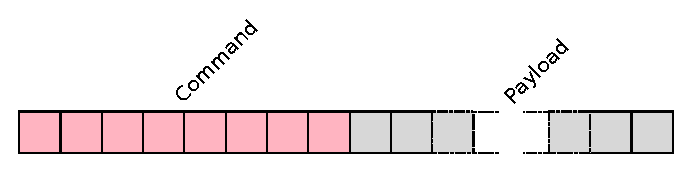
\includegraphics[width=.6\linewidth]{graphics/rxtx_payload.eps}
	\caption[Reading a payload on the nRF24L01.]{Bits written to and received from the \texttt{nRFM} when reading a payload. \texttt{Command} specifies the command given and \texttt{Payload} is the bits written from the \texttt{nRFM}.}
	\label{fig:rxtx_payload}
\end{figure}

Listing \ref{code:rf_read_payload} shows how a payload of 32 bytes is read in C code. 
Line 5 defines the input and output buffers and line 6 assigns the read payload command to the first byte of the output buffer.
33 bytes of data is sent in line 7-8, this is needed in order to create the clock signal for the \texttt{nRFM}, when it sends the 32 bytes payload.
The payload is also read and assigned to the input buffer in line 7-8.
Line 9-12 extracts the 32 bytes payload and ignores the first byte sent from the \texttt{nRFM}, which is the value of the \texttt{STATUS} register.

\begin{listing}[!h]
\begin{minted}{c}
#define R_RX_PAYLOAD       0b01100001
#define PAYLOAD_SIZE       32

void RF_read(XSpiPs *SPI_inst, u8 *buffer){
	u8 input_buffer[PAYLOAD_SIZE+1], output_buffer[PAYLOAD_SIZE+1];
	output_buffer[0] = R_RX_PAYLOAD;
	XSpiPs_PolledTransfer(SPI_inst, output_buffer, input_buffer, @$\Rightarrow$@
		PAYLOAD_SIZE+1);
	int i;
	for(i = 1; i < PAYLOAD_SIZE+1; i++){
		buffer[i-1] = input_buffer[i];
	}
}
\end{minted}
\caption[C function that reads 32 bytes payload from the nRFM]{Implementation of a C function that reads 32 bytes payload from the \texttt{nRFM}. Macros are shown for clarity.}
\label{code:rf_read_payload}
\end{listing}

\subsubsection{PWM Generation} % (fold)
\label{ssub:pwm_generation}
In order to generate the two needed PWM signals from the MicroZed an IP core must be made in VHDL.
As described the IP core needs to be able to switch the PWM signal between channel \texttt{A} and \texttt{B} and have a programmable duty cycle.
It also needs to have a top signal that indicates the center of the PWM pulse.
The designed PWM generator IP core has three inputs and three outputs as illustrated in figure \ref{fig:pwm_gen_component}.
\begin{figure}[h]
	\centering
	\includegraphics[width=.4\linewidth]{graphics/pwm_generator}
	\caption{Input and output signals of the PWM generator component.}
	\label{fig:pwm_gen_component}
\end{figure}
A counter is incremented to a high limit and decremented to zero using a state machine.
The high limit for the counter when using the MicroZed and a PWM frequency of 22KHz is calculated by:
\begin{equation}
	H_{limit} = \frac{F_{Microzed}}{F_{PWM}\cdot 2} = \frac{100\cdot 10^6}{22\cdot 10^3 \cdot 2} = 2272.7 \simeq 2273
\end{equation}
Where $H_{limit}$ is the high counting limit, $F_{MicroZed}$ and $F_{PWM}$ are the frequencies of the MicroZed and the PWM, respectively. 
The PWM output will be set \texttt{high}, when the counter value is greater than a compare value.
Using this mechanism the duty cycle of the PWM can be controlled through the compare value.
The compare value for a 50\% duty cycle should be calculated using:
\begin{equation}
	Compare = (1 - D) \cdot H_{limit} = (1 - 0.5) \cdot 2273 = 1136
\end{equation}
Where $Compare$ is the compare value and $D$ is the wanted duty cycle ratio.

The described mechanism is illustrated in figure \ref{sfig:pwm_gen_int}, where the top signal is simply set \texttt{high}, when the counter reaches its high limit.

\begin{figure}
    \centering
    \begin{subfigure}[b]{0.45\textwidth}
        %% This file was created by matlab2tikz.
%
%The latest updates can be retrieved from
%  http://www.mathworks.com/matlabcentral/fileexchange/22022-matlab2tikz-matlab2tikz
%where you can also make suggestions and rate matlab2tikz.
%
\definecolor{mycolor1}{rgb}{0.00000,0.44700,0.74100}%
\definecolor{mycolor2}{rgb}{0.85000,0.32500,0.09800}%
\definecolor{mycolor3}{rgb}{0.92900,0.69400,0.12500}%
\definecolor{mycolor4}{rgb}{0.49400,0.18400,0.55600}%

%
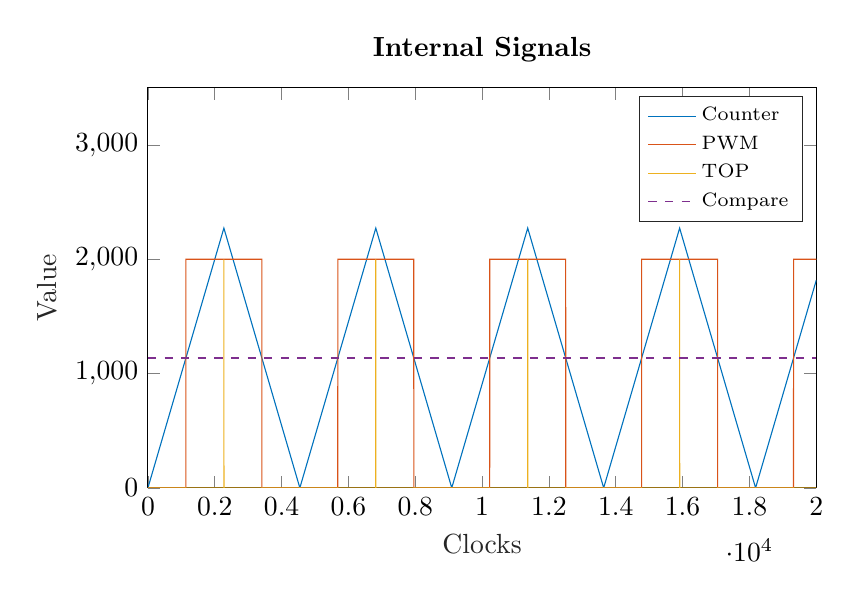
\begin{tikzpicture}

\begin{axis}[%
width=.70\textwidth,
height=2in,
at={(0.758in,0.481in)},
scale only axis,
xmin=0,
xmax=20000,
xlabel style={font=\color{white!15!black}},
xlabel={Clocks},
ymin=0,
ymax=3500,
ylabel style={font=\color{white!15!black}},
ylabel={Value},
axis background/.style={fill=white},
title style={font=\bfseries},
title={Internal Signals},
legend style={legend cell align=left,  align=left, font=\scriptsize, draw=white!15!black}
]
\addplot [color=mycolor1]
  table[row sep=crcr]{%
0	0\\
2273.08333638863	2273\\
4546.16667277727	0\\
6819.2500091659	2273\\
9092.33334555454	0\\
11365.4166819432	2273\\
13638.5000183318	0\\
15911.5833547204	2273\\
18184.6666911091	0\\
20000.7332722273	1816.79929577465\\
};
\addlegendentry{Counter}

\addplot [color=mycolor2]
  table[row sep=crcr]{%
0	0\\
1135.0416131989	0\\
1137.04168652612	2000\\
3409.12498625115	2000\\
3411.12505957837	0\\
5681.20828597617	0\\
5683.20835930339	2000\\
7955.29165902841	2000\\
7957.29173235564	0\\
10227.3749587534	0\\
10229.3750320807	2000\\
12501.4583318057	2000\\
12503.4584051329	0\\
14773.5416315307	0\\
14775.5417048579	2000\\
17047.625004583	2000\\
17049.6250779102	0\\
19319.708304308	0\\
19321.7083776352	2000\\
20000.7332722273	2000\\
};
\addlegendentry{PWM}

\addplot [color=mycolor3]
  table[row sep=crcr]{%
0	0\\
2271.08326306141	0\\
2273.08333638863	2000\\
2275.08340971586	0\\
6817.24993583868	0\\
6819.2500091659	2000\\
6821.25008249313	0\\
11363.4166086159	0\\
11365.4166819432	2000\\
11367.4167552704	0\\
15909.5832813932	0\\
15911.5833547204	2000\\
15913.5834280477	0\\
20000.7332722273	0\\
};
\addlegendentry{TOP}

\addplot [color=mycolor4, dashed]
  table[row sep=crcr]{%
0	1136\\
20000	1136\\
};
\addlegendentry{Compare}

\end{axis}
\end{tikzpicture}%
        \caption{Internal VHDL signals illustrated by a Matlab plot.}
        \label{sfig:pwm_gen_int}
    \end{subfigure}
    \begin{subfigure}[b]{0.45\textwidth}
        %% This file was created by matlab2tikz.
%
%The latest updates can be retrieved from
%  http://www.mathworks.com/matlabcentral/fileexchange/22022-matlab2tikz-matlab2tikz
%where you can also make suggestions and rate matlab2tikz.
%
\definecolor{mycolor1}{rgb}{0.00000,0.44700,0.74100}%
%
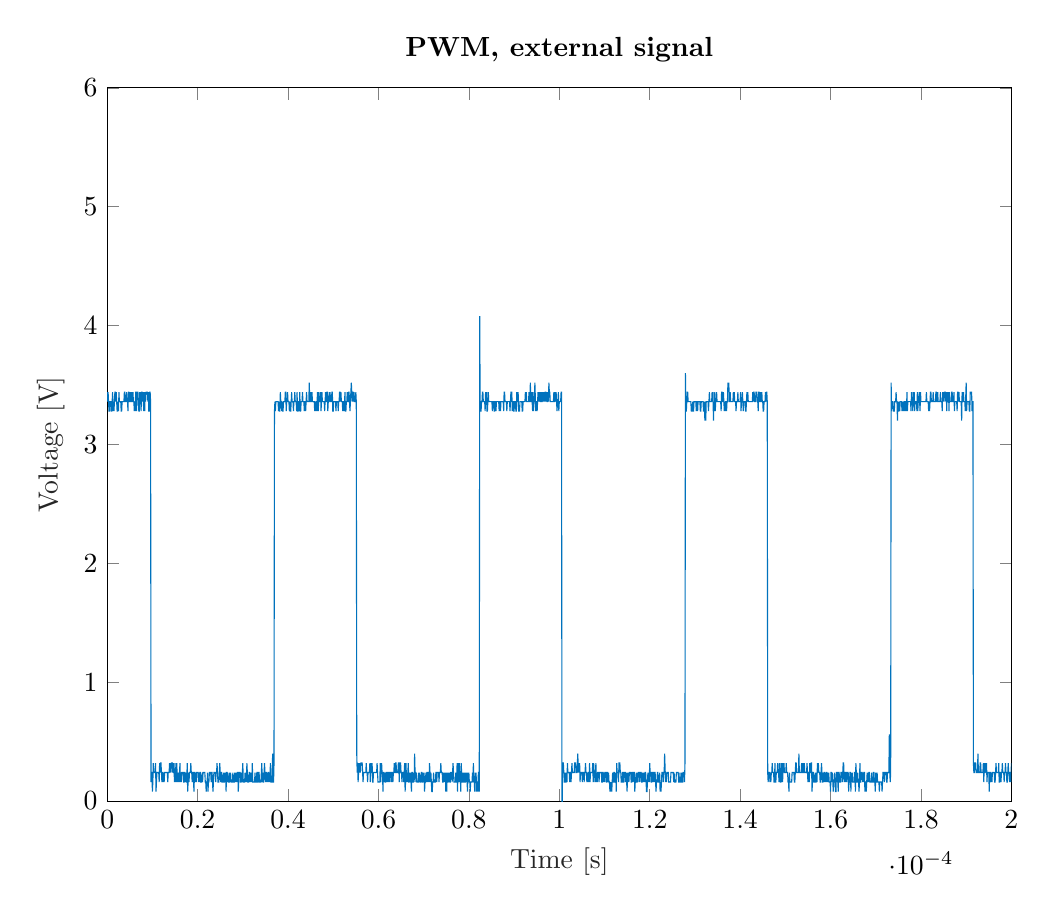
\begin{tikzpicture}

\begin{axis}[%
width=4.521in,
height=3.566in,
at={(0.758in,0.481in)},
scale only axis,
xmin=0,
xmax=0.0002,
xlabel style={font=\color{white!15!black}},
xlabel={Time [s]},
ymin=0,
ymax=6,
ylabel style={font=\color{white!15!black}},
ylabel={Voltage [V]},
axis background/.style={fill=white},
title style={font=\bfseries},
title={PWM, external signal}
]
\addplot [color=mycolor1, forget plot]
  table[row sep=crcr]{%
-1.00000000280431e-07	3.36\\
0	3.44\\
1.00000000280431e-07	3.36\\
1.99999999672684e-07	3.44\\
4.00000000233547e-07	3.28\\
4.999999996258e-07	3.28\\
5.99999999906231e-07	3.36\\
7.99999999578915e-07	3.36\\
8.99999999859347e-07	3.28\\
1.00000000013978e-06	3.28\\
1.19999999981246e-06	3.44\\
1.30000000009289e-06	3.28\\
1.40000000037332e-06	3.36\\
1.49999999976558e-06	3.28\\
1.70000000032644e-06	3.44\\
1.79999999971869e-06	3.44\\
1.89999999999912e-06	3.36\\
2.00000000027956e-06	3.44\\
2.19999999995224e-06	3.28\\
2.30000000023267e-06	3.28\\
2.39999999962492e-06	3.36\\
2.49999999990536e-06	3.28\\
2.60000000018579e-06	3.44\\
2.69999999957804e-06	3.36\\
3.00000000041933e-06	3.36\\
3.09999999981159e-06	3.28\\
3.20000000009202e-06	3.28\\
3.30000000037245e-06	3.36\\
3.69999999971782e-06	3.36\\
3.79999999999825e-06	3.44\\
3.90000000027868e-06	3.44\\
3.99999999967093e-06	3.36\\
4.2000000002318e-06	3.36\\
4.29999999962405e-06	3.44\\
4.39999999990448e-06	3.36\\
4.50000000018491e-06	3.36\\
4.59999999957716e-06	3.28\\
4.6999999998576e-06	3.44\\
4.80000000013803e-06	3.44\\
4.90000000041846e-06	3.36\\
4.99999999981071e-06	3.36\\
5.10000000009114e-06	3.44\\
5.20000000037157e-06	3.36\\
5.29999999976383e-06	3.36\\
5.40000000004426e-06	3.44\\
5.50000000032469e-06	3.36\\
5.59999999971694e-06	3.36\\
5.69999999999737e-06	3.44\\
5.80000000027781e-06	3.36\\
5.89999999967006e-06	3.36\\
5.99999999995049e-06	3.28\\
6.10000000023092e-06	3.36\\
6.19999999962317e-06	3.28\\
6.2999999999036e-06	3.44\\
6.40000000018404e-06	3.44\\
6.49999999957629e-06	3.28\\
6.59999999985672e-06	3.44\\
6.80000000041758e-06	3.44\\
7.00000000009027e-06	3.28\\
7.1000000003707e-06	3.28\\
7.19999999976295e-06	3.44\\
7.30000000004338e-06	3.36\\
7.40000000032381e-06	3.44\\
7.49999999971607e-06	3.28\\
7.5999999999965e-06	3.44\\
7.70000000027693e-06	3.44\\
7.79999999966918e-06	3.36\\
7.89999999994961e-06	3.44\\
8.0999999996223e-06	3.28\\
8.19999999990273e-06	3.44\\
8.30000000018316e-06	3.28\\
8.39999999957541e-06	3.44\\
8.49999999985585e-06	3.36\\
8.60000000013628e-06	3.44\\
8.90000000008939e-06	3.44\\
9.00000000036982e-06	3.36\\
9.09999999976208e-06	3.44\\
9.20000000004251e-06	3.28\\
9.30000000032294e-06	3.28\\
9.39999999971519e-06	3.44\\
9.49999999999562e-06	3.44\\
9.60000000027605e-06	3.36\\
9.69999999966831e-06	0.16\\
9.79999999994874e-06	0.24\\
9.90000000022917e-06	0.24\\
9.99999999962142e-06	0.0800000000000001\\
1.00999999999019e-05	0.16\\
1.02000000001823e-05	0.32\\
1.02999999995745e-05	0.24\\
1.06000000004158e-05	0.24\\
1.06999999998081e-05	0.32\\
1.08000000000885e-05	0.0800000000000001\\
1.09999999997612e-05	0.24\\
1.13999999999947e-05	0.24\\
1.15000000002752e-05	0.16\\
1.15999999996674e-05	0.32\\
1.16999999999479e-05	0.24\\
1.18000000002283e-05	0.32\\
1.18999999996205e-05	0.32\\
1.21000000001814e-05	0.16\\
1.21999999995737e-05	0.24\\
1.22999999998541e-05	0.24\\
1.24000000001345e-05	0.16\\
1.2500000000415e-05	0.24\\
1.25999999998072e-05	0.16\\
1.27000000000876e-05	0.24\\
1.32999999999939e-05	0.24\\
1.34000000002743e-05	0.16\\
1.34999999996666e-05	0.24\\
1.37000000002274e-05	0.24\\
1.37999999996197e-05	0.32\\
1.38999999999001e-05	0.24\\
1.40000000001805e-05	0.32\\
1.40999999995728e-05	0.24\\
1.41999999998532e-05	0.32\\
1.44000000004141e-05	0.32\\
1.44999999998063e-05	0.24\\
1.46000000000868e-05	0.32\\
1.47000000003672e-05	0.24\\
1.47999999997595e-05	0.24\\
1.49000000000399e-05	0.16\\
1.50000000003203e-05	0.32\\
1.5199999999993e-05	0.16\\
1.53999999996657e-05	0.32\\
1.54999999999461e-05	0.16\\
1.56000000002265e-05	0.24\\
1.56999999996188e-05	0.16\\
1.57999999998992e-05	0.24\\
1.59000000001797e-05	0.16\\
1.60999999998523e-05	0.32\\
1.62000000001328e-05	0.16\\
1.63000000004132e-05	0.24\\
1.63999999998055e-05	0.16\\
1.65000000000859e-05	0.24\\
1.6800000000039e-05	0.24\\
1.69000000003194e-05	0.16\\
1.69999999997117e-05	0.16\\
1.70999999999921e-05	0.24\\
1.72000000002726e-05	0.24\\
1.72999999996648e-05	0.16\\
1.73999999999452e-05	0.24\\
1.75000000002257e-05	0.16\\
1.75999999996179e-05	0.16\\
1.76999999998984e-05	0.32\\
1.78000000001788e-05	0.0800000000000001\\
1.79999999998515e-05	0.24\\
1.81000000001319e-05	0.16\\
1.82000000004123e-05	0.24\\
1.8400000000085e-05	0.24\\
1.85000000003654e-05	0.32\\
1.85999999997577e-05	0.24\\
1.87000000000381e-05	0.24\\
1.88000000003186e-05	0.16\\
1.88999999997108e-05	0.24\\
1.89999999999912e-05	0.24\\
1.91999999996639e-05	0.0800000000000001\\
1.92999999999444e-05	0.24\\
1.94000000002248e-05	0.24\\
1.9499999999617e-05	0.16\\
1.95999999998975e-05	0.24\\
1.97000000001779e-05	0.16\\
1.97999999995702e-05	0.24\\
2.01000000004115e-05	0.24\\
2.01999999998037e-05	0.16\\
2.03000000000841e-05	0.24\\
2.04000000003646e-05	0.16\\
2.04999999997568e-05	0.24\\
2.06000000000373e-05	0.24\\
2.07000000003177e-05	0.16\\
2.08999999999904e-05	0.16\\
2.10000000002708e-05	0.24\\
2.10999999996631e-05	0.16\\
2.11999999999435e-05	0.24\\
2.1600000000177e-05	0.24\\
2.16999999995693e-05	0.16\\
2.17999999998497e-05	0.16\\
2.19000000001301e-05	0.0800000000000001\\
2.20000000004106e-05	0.16\\
2.20999999998028e-05	0.16\\
2.22000000000833e-05	0.24\\
2.23000000003637e-05	0.0800000000000001\\
2.23999999997559e-05	0.16\\
2.25000000000364e-05	0.16\\
2.26000000003168e-05	0.24\\
2.29000000002699e-05	0.24\\
2.29999999996622e-05	0.16\\
2.30999999999426e-05	0.24\\
2.3200000000223e-05	0.24\\
2.33999999998957e-05	0.0800000000000001\\
2.35999999995684e-05	0.24\\
2.39000000004097e-05	0.24\\
2.3999999999802e-05	0.16\\
2.41000000000824e-05	0.24\\
2.42000000003628e-05	0.24\\
2.42999999997551e-05	0.32\\
2.45000000003159e-05	0.16\\
2.46999999999886e-05	0.16\\
2.48999999996613e-05	0.32\\
2.51000000002222e-05	0.16\\
2.51999999996144e-05	0.24\\
2.52999999998949e-05	0.24\\
2.54000000001753e-05	0.16\\
2.5599999999848e-05	0.16\\
2.57000000001284e-05	0.24\\
2.58000000004088e-05	0.16\\
2.58999999998011e-05	0.16\\
2.60000000000815e-05	0.24\\
2.61000000003619e-05	0.16\\
2.61999999997542e-05	0.24\\
2.63000000000346e-05	0.0800000000000001\\
2.64000000003151e-05	0.24\\
2.64999999997073e-05	0.24\\
2.65999999999877e-05	0.16\\
2.67000000002682e-05	0.24\\
2.67999999996604e-05	0.16\\
2.70000000002213e-05	0.16\\
2.70999999996135e-05	0.24\\
2.7199999999894e-05	0.16\\
2.73000000001744e-05	0.24\\
2.73999999995667e-05	0.16\\
2.7700000000408e-05	0.16\\
2.77999999998002e-05	0.24\\
2.79000000000806e-05	0.16\\
2.80999999997533e-05	0.16\\
2.82000000000338e-05	0.24\\
2.83000000003142e-05	0.16\\
2.83999999997064e-05	0.24\\
2.84999999999869e-05	0.16\\
2.86000000002673e-05	0.24\\
2.86999999996596e-05	0.16\\
2.879999999994e-05	0.24\\
2.89000000002204e-05	0.24\\
2.89999999996127e-05	0.0800000000000001\\
2.92000000001735e-05	0.24\\
2.93999999998462e-05	0.24\\
2.95000000001266e-05	0.16\\
2.96000000004071e-05	0.16\\
2.96999999997993e-05	0.24\\
2.98000000000798e-05	0.16\\
2.99999999997524e-05	0.32\\
3.01000000000329e-05	0.16\\
3.0399999999986e-05	0.16\\
3.05000000002664e-05	0.24\\
3.05999999996587e-05	0.16\\
3.06999999999391e-05	0.24\\
3.08000000002195e-05	0.16\\
3.08999999996118e-05	0.32\\
3.11000000001727e-05	0.16\\
3.12999999998453e-05	0.16\\
3.14000000001258e-05	0.24\\
3.15000000004062e-05	0.24\\
3.15999999997985e-05	0.16\\
3.17000000000789e-05	0.24\\
3.18000000003593e-05	0.16\\
3.18999999997516e-05	0.24\\
3.2000000000032e-05	0.16\\
3.21000000003124e-05	0.32\\
3.21999999997047e-05	0.16\\
3.25999999999382e-05	0.16\\
3.27000000002187e-05	0.24\\
3.27999999996109e-05	0.16\\
3.30000000001718e-05	0.16\\
3.3099999999564e-05	0.24\\
3.31999999998445e-05	0.24\\
3.33000000001249e-05	0.16\\
3.34000000004053e-05	0.16\\
3.34999999997976e-05	0.24\\
3.3600000000078e-05	0.24\\
3.37000000003584e-05	0.16\\
3.40000000003116e-05	0.16\\
3.41999999999842e-05	0.32\\
3.43000000002647e-05	0.16\\
3.43999999996569e-05	0.24\\
3.44999999999374e-05	0.16\\
3.46000000002178e-05	0.16\\
3.47999999998905e-05	0.32\\
3.49999999995632e-05	0.16\\
3.50999999998436e-05	0.24\\
3.5200000000124e-05	0.24\\
3.53000000004045e-05	0.16\\
3.53999999997967e-05	0.24\\
3.55000000000771e-05	0.16\\
3.56000000003576e-05	0.24\\
3.56999999997498e-05	0.24\\
3.58000000000303e-05	0.16\\
3.59000000003107e-05	0.24\\
3.59999999997029e-05	0.16\\
3.60999999999834e-05	0.32\\
3.62000000002638e-05	0.16\\
3.63999999999365e-05	0.16\\
3.65000000002169e-05	0.24\\
3.65999999996092e-05	0.4\\
3.66999999998896e-05	0.16\\
3.680000000017e-05	0.16\\
3.68999999995623e-05	0.32\\
3.69999999998427e-05	3.28\\
3.71000000001231e-05	3.36\\
3.72000000004036e-05	3.28\\
3.72999999997958e-05	3.36\\
3.78000000003098e-05	3.36\\
3.78999999997021e-05	3.28\\
3.79999999999825e-05	3.36\\
3.81000000002629e-05	3.28\\
3.81999999996552e-05	3.28\\
3.82999999999356e-05	3.44\\
3.8400000000216e-05	3.36\\
3.84999999996083e-05	3.36\\
3.85999999998887e-05	3.28\\
3.87000000001692e-05	3.36\\
3.87999999995614e-05	3.28\\
3.88999999998418e-05	3.28\\
3.90000000001223e-05	3.36\\
3.93000000000754e-05	3.36\\
3.94000000003558e-05	3.44\\
3.94999999997481e-05	3.44\\
3.96000000000285e-05	3.28\\
3.97000000003089e-05	3.36\\
3.97999999997012e-05	3.36\\
3.98999999999816e-05	3.44\\
4.0000000000262e-05	3.36\\
4.01999999999347e-05	3.36\\
4.03000000002152e-05	3.28\\
4.03999999996074e-05	3.36\\
4.04999999998878e-05	3.28\\
4.06000000001683e-05	3.28\\
4.0799999999841e-05	3.44\\
4.09000000001214e-05	3.36\\
4.10999999997941e-05	3.36\\
4.12000000000745e-05	3.28\\
4.13000000003549e-05	3.36\\
4.13999999997472e-05	3.36\\
4.15000000000276e-05	3.44\\
4.16000000003081e-05	3.36\\
4.17999999999807e-05	3.36\\
4.19000000002612e-05	3.28\\
4.19999999996534e-05	3.44\\
4.20999999999339e-05	3.28\\
4.22000000002143e-05	3.28\\
4.22999999996065e-05	3.36\\
4.2399999999887e-05	3.36\\
4.25000000001674e-05	3.28\\
4.25999999995597e-05	3.44\\
4.26999999998401e-05	3.28\\
4.28000000001205e-05	3.28\\
4.2900000000401e-05	3.36\\
4.31000000000736e-05	3.36\\
4.32000000003541e-05	3.44\\
4.32999999997463e-05	3.36\\
4.35000000003072e-05	3.36\\
4.35999999996994e-05	3.28\\
4.36999999999799e-05	3.36\\
4.38000000002603e-05	3.36\\
4.38999999996526e-05	3.28\\
4.41000000002134e-05	3.44\\
4.41999999996057e-05	3.36\\
4.45999999998392e-05	3.36\\
4.47000000001196e-05	3.52\\
4.48000000004001e-05	3.36\\
4.48999999997923e-05	3.36\\
4.50000000000728e-05	3.44\\
4.51000000003532e-05	3.36\\
4.51999999997454e-05	3.36\\
4.53000000000259e-05	3.44\\
4.54000000003063e-05	3.36\\
4.57999999996517e-05	3.36\\
4.58999999999321e-05	3.28\\
4.60000000002125e-05	3.36\\
4.60999999996048e-05	3.28\\
4.61999999998852e-05	3.36\\
4.63000000001657e-05	3.36\\
4.63999999995579e-05	3.28\\
4.64999999998383e-05	3.44\\
4.67000000003992e-05	3.28\\
4.67999999997915e-05	3.44\\
4.69000000000719e-05	3.36\\
4.70999999997446e-05	3.36\\
4.7200000000025e-05	3.44\\
4.73000000003054e-05	3.28\\
4.74999999999781e-05	3.44\\
4.76000000002585e-05	3.36\\
4.79999999996039e-05	3.36\\
4.80999999998843e-05	3.28\\
4.8299999999557e-05	3.44\\
4.83999999998375e-05	3.36\\
4.85000000001179e-05	3.36\\
4.86000000003983e-05	3.44\\
4.86999999997906e-05	3.44\\
4.8800000000071e-05	3.28\\
4.89000000003514e-05	3.36\\
4.89999999997437e-05	3.36\\
4.91000000000241e-05	3.44\\
4.92000000003046e-05	3.36\\
4.92999999996968e-05	3.44\\
4.93999999999772e-05	3.36\\
4.95999999996499e-05	3.36\\
4.96999999999304e-05	3.44\\
4.98000000002108e-05	3.44\\
4.9899999999603e-05	3.28\\
4.99999999998835e-05	3.28\\
5.01000000001639e-05	3.36\\
5.05000000003974e-05	3.36\\
5.05999999997897e-05	3.28\\
5.07000000000701e-05	3.36\\
5.10000000000232e-05	3.36\\
5.11000000003037e-05	3.28\\
5.11999999996959e-05	3.36\\
5.12999999999764e-05	3.36\\
5.14000000002568e-05	3.44\\
5.1499999999649e-05	3.44\\
5.15999999999295e-05	3.36\\
5.17000000002099e-05	3.44\\
5.17999999996022e-05	3.36\\
5.2000000000163e-05	3.36\\
5.21000000004435e-05	3.28\\
5.21999999998357e-05	3.36\\
5.23000000001161e-05	3.36\\
5.24000000003966e-05	3.28\\
5.26000000000693e-05	3.44\\
5.27000000003497e-05	3.28\\
5.27999999997419e-05	3.28\\
5.29000000000224e-05	3.36\\
5.30000000003028e-05	3.36\\
5.30999999996951e-05	3.44\\
5.31999999999755e-05	3.36\\
5.33000000002559e-05	3.36\\
5.33999999996482e-05	3.44\\
5.34999999999286e-05	3.44\\
5.36999999996013e-05	3.28\\
5.40000000004426e-05	3.52\\
5.42000000001153e-05	3.36\\
5.43000000003957e-05	3.44\\
5.4399999999788e-05	3.44\\
5.45000000000684e-05	3.36\\
5.46000000003488e-05	3.44\\
5.46999999997411e-05	3.36\\
5.49000000003019e-05	3.36\\
5.49999999996942e-05	3.44\\
5.50999999999746e-05	3.36\\
5.5200000000255e-05	0.4\\
5.52999999996473e-05	0.24\\
5.53999999999277e-05	0.32\\
5.55000000002082e-05	0.16\\
5.56999999998808e-05	0.32\\
5.58000000001613e-05	0.24\\
5.59000000004417e-05	0.32\\
5.5999999999834e-05	0.24\\
5.61000000001144e-05	0.32\\
5.64000000000675e-05	0.32\\
5.65999999997402e-05	0.16\\
5.67000000000206e-05	0.24\\
5.71999999996464e-05	0.24\\
5.72999999999269e-05	0.32\\
5.74000000002073e-05	0.24\\
5.74999999995995e-05	0.24\\
5.759999999988e-05	0.16\\
5.77000000001604e-05	0.24\\
5.80000000001135e-05	0.24\\
5.81000000003939e-05	0.32\\
5.81999999997862e-05	0.16\\
5.83000000000666e-05	0.32\\
5.84000000003471e-05	0.24\\
5.84999999997393e-05	0.24\\
5.86000000000197e-05	0.32\\
5.87000000003002e-05	0.16\\
5.87999999996924e-05	0.16\\
5.88999999999729e-05	0.24\\
5.96000000001595e-05	0.24\\
5.970000000044e-05	0.32\\
5.99000000001126e-05	0.16\\
6.03000000003462e-05	0.16\\
6.03999999997384e-05	0.32\\
6.05000000000189e-05	0.16\\
6.06999999996916e-05	0.32\\
6.0799999999972e-05	0.24\\
6.09000000002524e-05	0.24\\
6.09999999996447e-05	0.0800000000000001\\
6.10999999999251e-05	0.24\\
6.12000000002055e-05	0.24\\
6.12999999995978e-05	0.16\\
6.13999999998782e-05	0.24\\
6.15000000001586e-05	0.16\\
6.16000000004391e-05	0.16\\
6.16999999998313e-05	0.24\\
6.18000000001118e-05	0.24\\
6.19000000003922e-05	0.16\\
6.19999999997844e-05	0.24\\
6.21000000000649e-05	0.24\\
6.22000000003453e-05	0.16\\
6.22999999997376e-05	0.24\\
6.2400000000018e-05	0.24\\
6.25000000002984e-05	0.16\\
6.25999999996907e-05	0.24\\
6.28000000002515e-05	0.24\\
6.28999999996438e-05	0.16\\
6.29999999999242e-05	0.24\\
6.31000000002047e-05	0.24\\
6.31999999995969e-05	0.16\\
6.32999999998773e-05	0.24\\
6.34000000001578e-05	0.24\\
6.35000000004382e-05	0.32\\
6.35999999998305e-05	0.24\\
6.37000000001109e-05	0.24\\
6.38000000003913e-05	0.32\\
6.38999999997836e-05	0.32\\
6.4000000000064e-05	0.24\\
6.43000000000171e-05	0.24\\
6.44000000002976e-05	0.32\\
6.44999999996898e-05	0.32\\
6.45999999999702e-05	0.16\\
6.47000000002507e-05	0.32\\
6.48999999999234e-05	0.32\\
6.50000000002038e-05	0.24\\
6.5099999999596e-05	0.24\\
6.51999999998765e-05	0.16\\
6.53000000001569e-05	0.24\\
6.54999999998296e-05	0.24\\
6.560000000011e-05	0.16\\
6.57999999997827e-05	0.32\\
6.59000000000631e-05	0.0800000000000001\\
6.60000000003436e-05	0.16\\
6.60999999997358e-05	0.32\\
6.62000000000162e-05	0.16\\
6.63000000002967e-05	0.24\\
6.63999999996889e-05	0.16\\
6.66000000002498e-05	0.32\\
6.6699999999642e-05	0.16\\
6.67999999999225e-05	0.16\\
6.69000000002029e-05	0.24\\
6.69999999995952e-05	0.16\\
6.70999999998756e-05	0.24\\
6.73000000004365e-05	0.0800000000000001\\
6.73999999998287e-05	0.24\\
6.75000000001091e-05	0.24\\
6.76000000003896e-05	0.16\\
6.76999999997818e-05	0.16\\
6.78000000000623e-05	0.24\\
6.79000000003427e-05	0.16\\
6.79999999997349e-05	0.4\\
6.81000000000154e-05	0.24\\
6.82000000002958e-05	0.24\\
6.82999999996881e-05	0.16\\
6.83999999999685e-05	0.24\\
6.85000000002489e-05	0.16\\
6.8800000000202e-05	0.16\\
6.88999999995943e-05	0.24\\
6.89999999998747e-05	0.16\\
6.91000000001551e-05	0.24\\
6.92000000004356e-05	0.16\\
6.94000000001083e-05	0.16\\
6.95000000003887e-05	0.24\\
6.95999999997809e-05	0.24\\
6.97000000000614e-05	0.16\\
6.98000000003418e-05	0.16\\
6.98999999997341e-05	0.24\\
7.00000000000145e-05	0.16\\
7.01000000002949e-05	0.24\\
7.01999999996872e-05	0.0800000000000001\\
7.02999999999676e-05	0.16\\
7.0400000000248e-05	0.16\\
7.04999999996403e-05	0.24\\
7.05999999999207e-05	0.16\\
7.07000000002012e-05	0.24\\
7.07999999995934e-05	0.24\\
7.08999999998738e-05	0.16\\
7.10000000001543e-05	0.24\\
7.11000000004347e-05	0.24\\
7.1199999999827e-05	0.16\\
7.13000000001074e-05	0.32\\
7.14999999997801e-05	0.16\\
7.16000000000605e-05	0.24\\
7.17999999997332e-05	0.0800000000000001\\
7.19000000000136e-05	0.0800000000000001\\
7.20000000002941e-05	0.16\\
7.20999999996863e-05	0.16\\
7.21999999999667e-05	0.24\\
7.23000000002472e-05	0.16\\
7.26000000002003e-05	0.16\\
7.26999999995925e-05	0.24\\
7.2799999999873e-05	0.24\\
7.29000000001534e-05	0.16\\
7.30000000004338e-05	0.24\\
7.33000000003869e-05	0.24\\
7.33999999997792e-05	0.16\\
7.35000000000596e-05	0.24\\
7.36999999997323e-05	0.24\\
7.38000000000127e-05	0.32\\
7.39000000002932e-05	0.24\\
7.40999999999659e-05	0.24\\
7.42000000002463e-05	0.16\\
7.42999999996385e-05	0.16\\
7.4399999999919e-05	0.24\\
7.45000000001994e-05	0.16\\
7.45999999995917e-05	0.24\\
7.46999999998721e-05	0.16\\
7.48000000001525e-05	0.24\\
7.4900000000433e-05	0.0800000000000001\\
7.49999999998252e-05	0.24\\
7.51000000001056e-05	0.0800000000000001\\
7.52000000003861e-05	0.24\\
7.52999999997783e-05	0.16\\
7.54000000000588e-05	0.16\\
7.55000000003392e-05	0.24\\
7.55999999997314e-05	0.16\\
7.57000000000119e-05	0.24\\
7.58000000002923e-05	0.16\\
7.58999999996846e-05	0.16\\
7.5999999999965e-05	0.24\\
7.61999999996377e-05	0.24\\
7.62999999999181e-05	0.16\\
7.64999999995908e-05	0.32\\
7.67000000001516e-05	0.16\\
7.70000000001048e-05	0.16\\
7.71000000003852e-05	0.24\\
7.71999999997774e-05	0.16\\
7.73000000000579e-05	0.16\\
7.74000000003383e-05	0.32\\
7.74999999997306e-05	0.0800000000000001\\
7.7600000000011e-05	0.32\\
7.77999999996837e-05	0.16\\
7.78999999999641e-05	0.32\\
7.80000000002445e-05	0.16\\
7.80999999996368e-05	0.24\\
7.81999999999172e-05	0.0800000000000001\\
7.83000000001977e-05	0.32\\
7.84999999998703e-05	0.16\\
7.86000000001508e-05	0.16\\
7.87000000004312e-05	0.24\\
7.87999999998235e-05	0.16\\
7.89000000001039e-05	0.16\\
7.90000000003843e-05	0.24\\
7.90999999997766e-05	0.16\\
7.9200000000057e-05	0.16\\
7.93000000003374e-05	0.24\\
7.93999999997297e-05	0.16\\
7.95000000000101e-05	0.24\\
7.96999999996828e-05	0.0800000000000001\\
7.97999999999632e-05	0.24\\
7.99000000002437e-05	0.16\\
7.99999999996359e-05	0.24\\
8.00999999999163e-05	0.16\\
8.02000000001968e-05	0.16\\
8.0299999999589e-05	0.0800000000000001\\
8.03999999998695e-05	0.16\\
8.06999999998226e-05	0.16\\
8.0800000000103e-05	0.24\\
8.09000000003834e-05	0.16\\
8.09999999997757e-05	0.32\\
8.11000000000561e-05	0.16\\
8.12000000003366e-05	0.16\\
8.12999999997288e-05	0.0800000000000001\\
8.14000000000092e-05	0.24\\
8.15000000002897e-05	0.16\\
8.15999999996819e-05	0.24\\
8.16999999999624e-05	0.0800000000000001\\
8.18000000002428e-05	0.16\\
8.1899999999635e-05	0.16\\
8.19999999999155e-05	0.0800000000000001\\
8.21000000001959e-05	0.24\\
8.21999999995882e-05	0.24\\
8.22999999998686e-05	0.0800000000000001\\
8.2400000000149e-05	4.08\\
8.25000000004295e-05	3.28\\
8.27000000001021e-05	3.28\\
8.28000000003826e-05	3.36\\
8.28999999997748e-05	3.36\\
8.30000000000553e-05	3.44\\
8.31000000003357e-05	3.44\\
8.31999999997279e-05	3.36\\
8.34999999996811e-05	3.36\\
8.35999999999615e-05	3.28\\
8.37000000002419e-05	3.44\\
8.37999999996342e-05	3.36\\
8.38999999999146e-05	3.44\\
8.4000000000195e-05	3.28\\
8.40999999995873e-05	3.28\\
8.43000000001481e-05	3.44\\
8.44000000004286e-05	3.36\\
8.50999999997271e-05	3.36\\
8.52000000000075e-05	3.28\\
8.53000000002879e-05	3.36\\
8.54999999999606e-05	3.36\\
8.5600000000241e-05	3.28\\
8.56999999996333e-05	3.28\\
8.57999999999137e-05	3.36\\
8.59000000001942e-05	3.36\\
8.59999999995864e-05	3.28\\
8.60999999998668e-05	3.36\\
8.66000000003808e-05	3.36\\
8.66999999997731e-05	3.28\\
8.68000000000535e-05	3.36\\
8.69000000003339e-05	3.36\\
8.69999999997262e-05	3.28\\
8.71000000000066e-05	3.36\\
8.75999999996324e-05	3.36\\
8.76999999999128e-05	3.28\\
8.78000000001933e-05	3.44\\
8.78999999995855e-05	3.44\\
8.7999999999866e-05	3.36\\
8.82999999998191e-05	3.36\\
8.84000000000995e-05	3.28\\
8.85000000003799e-05	3.36\\
8.90000000000057e-05	3.36\\
8.91000000002862e-05	3.28\\
8.92999999999589e-05	3.44\\
8.94999999996315e-05	3.44\\
8.9599999999912e-05	3.28\\
8.97000000001924e-05	3.36\\
8.97999999995847e-05	3.36\\
8.98999999998651e-05	3.28\\
9.00000000001455e-05	3.28\\
9.0100000000426e-05	3.36\\
9.03000000000986e-05	3.36\\
9.04000000003791e-05	3.28\\
9.04999999997713e-05	3.28\\
9.06000000000518e-05	3.44\\
9.07000000003322e-05	3.36\\
9.07999999997244e-05	3.36\\
9.09000000000049e-05	3.44\\
9.10000000002853e-05	3.28\\
9.1199999999958e-05	3.28\\
9.13000000002384e-05	3.36\\
9.16999999995838e-05	3.36\\
9.17999999998642e-05	3.28\\
9.19000000001446e-05	3.28\\
9.20000000004251e-05	3.36\\
9.23999999997704e-05	3.36\\
9.25000000000509e-05	3.44\\
9.26000000003313e-05	3.36\\
9.26999999997236e-05	3.44\\
9.2800000000004e-05	3.36\\
9.32000000002375e-05	3.36\\
9.32999999996298e-05	3.44\\
9.33999999999102e-05	3.36\\
9.35000000001907e-05	3.36\\
9.35999999995829e-05	3.52\\
9.36999999998633e-05	3.36\\
9.38000000001438e-05	3.36\\
9.39000000004242e-05	3.44\\
9.41000000000969e-05	3.28\\
9.42000000003773e-05	3.44\\
9.42999999997696e-05	3.28\\
9.440000000005e-05	3.36\\
9.45000000003304e-05	3.36\\
9.45999999997227e-05	3.52\\
9.48000000002835e-05	3.28\\
9.48999999996758e-05	3.36\\
9.49999999999562e-05	3.36\\
9.51000000002367e-05	3.28\\
9.52999999999093e-05	3.44\\
9.54000000001898e-05	3.36\\
9.5499999999582e-05	3.44\\
9.55999999998625e-05	3.36\\
9.57000000001429e-05	3.44\\
9.58000000004233e-05	3.36\\
9.58999999998156e-05	3.36\\
9.6000000000096e-05	3.44\\
9.61000000003764e-05	3.36\\
9.61999999997687e-05	3.36\\
9.63000000000491e-05	3.44\\
9.64000000003296e-05	3.36\\
9.64999999997218e-05	3.44\\
9.66000000000022e-05	3.36\\
9.67000000002827e-05	3.44\\
9.67999999996749e-05	3.36\\
9.68999999999554e-05	3.44\\
9.70000000002358e-05	3.44\\
9.7099999999628e-05	3.36\\
9.71999999999085e-05	3.44\\
9.73000000001889e-05	3.36\\
9.73999999995812e-05	3.36\\
9.74999999998616e-05	3.44\\
9.7600000000142e-05	3.36\\
9.77000000004224e-05	3.52\\
9.77999999998147e-05	3.44\\
9.79000000000951e-05	3.44\\
9.80000000003756e-05	3.36\\
9.8699999999674e-05	3.36\\
9.87999999999545e-05	3.44\\
9.89000000002349e-05	3.36\\
9.89999999996272e-05	3.36\\
9.90999999999076e-05	3.44\\
9.9200000000188e-05	3.36\\
9.92999999995803e-05	3.44\\
9.95000000001411e-05	3.28\\
9.96000000004216e-05	3.36\\
9.96999999998138e-05	3.36\\
9.98000000000943e-05	3.44\\
9.99000000003747e-05	3.28\\
9.99999999997669e-05	3.36\\
0.00010029999999972	3.36\\
0.0001004	3.44\\
0.000100500000000281	3.44\\
0.000100599999999673	-0.24\\
0.000100699999999954	0.24\\
0.000100800000000234	0.32\\
0.000100899999999626	0.32\\
0.000101100000000187	0.16\\
0.000101199999999579	0.16\\
0.00010129999999986	0.24\\
0.00010140000000014	0.16\\
0.000101500000000421	0.16\\
0.000101599999999813	0.24\\
0.000101700000000093	0.16\\
0.000101800000000374	0.32\\
0.000101899999999766	0.24\\
0.000102199999999719	0.24\\
0.0001023	0.16\\
0.00010240000000028	0.24\\
0.000102499999999672	0.24\\
0.000102599999999953	0.16\\
0.000102799999999625	0.32\\
0.000102899999999906	0.24\\
0.000103300000000139	0.24\\
0.00010340000000042	0.32\\
0.000103600000000093	0.32\\
0.000103700000000373	0.24\\
0.000103900000000046	0.24\\
0.000104099999999718	0.4\\
0.000104199999999999	0.24\\
0.000104300000000279	0.32\\
0.000104399999999671	0.24\\
0.000104499999999952	0.32\\
0.000104600000000232	0.16\\
0.000104699999999625	0.24\\
0.000104999999999578	0.24\\
0.000105099999999858	0.16\\
0.000105200000000139	0.24\\
0.000105399999999811	0.24\\
0.000105500000000092	0.16\\
0.000105600000000372	0.24\\
0.000105699999999764	0.24\\
0.000105800000000045	0.32\\
0.000105900000000325	0.24\\
0.000105999999999717	0.24\\
0.000106099999999998	0.16\\
0.000106200000000278	0.24\\
0.000106299999999671	0.16\\
0.000106399999999951	0.24\\
0.000106500000000231	0.24\\
0.000106599999999624	0.16\\
0.000106699999999904	0.32\\
0.000106800000000185	0.16\\
0.000106899999999577	0.24\\
0.00010729999999981	0.24\\
0.000107400000000091	0.32\\
0.000107500000000371	0.16\\
0.000107599999999763	0.32\\
0.000107700000000044	0.24\\
0.000107800000000324	0.24\\
0.000107899999999717	0.16\\
0.000108100000000277	0.32\\
0.00010819999999967	0.16\\
0.00010829999999995	0.24\\
0.000108400000000231	0.16\\
0.000108499999999623	0.24\\
0.000108700000000184	0.24\\
0.000108799999999576	0.16\\
0.000108899999999856	0.24\\
0.00010930000000009	0.24\\
0.00010940000000037	0.16\\
0.000109499999999763	0.16\\
0.000109600000000043	0.24\\
0.000109700000000323	0.24\\
0.000109799999999716	0.16\\
0.000109899999999996	0.24\\
0.000110000000000277	0.16\\
0.000110099999999669	0.24\\
0.00011030000000023	0.24\\
0.000110399999999622	0.16\\
0.000110499999999902	0.16\\
0.000110600000000183	0.24\\
0.000110699999999575	0.24\\
0.000110799999999855	0.16\\
0.000110900000000136	0.24\\
0.000111000000000416	0.16\\
0.000111099999999809	0.16\\
0.000111200000000089	0.0800000000000001\\
0.000111300000000369	0.16\\
0.000111399999999762	0.0800000000000001\\
0.000111500000000042	0.16\\
0.000111600000000323	0.0800000000000001\\
0.000111799999999995	0.24\\
0.000111900000000276	0.16\\
0.000111999999999668	0.16\\
0.000112099999999948	0.24\\
0.000112200000000229	0.24\\
0.000112299999999621	0.16\\
0.000112399999999901	0.16\\
0.000112500000000182	0.24\\
0.000112599999999574	0.0800000000000001\\
0.000112699999999855	0.32\\
0.000112800000000135	0.24\\
0.000112999999999808	0.24\\
0.000113100000000088	0.16\\
0.000113200000000369	0.32\\
0.000113400000000041	0.32\\
0.000113500000000322	0.24\\
0.000113599999999714	0.24\\
0.000113699999999994	0.16\\
0.000113899999999667	0.16\\
0.000113999999999947	0.24\\
0.000114100000000228	0.24\\
0.00011419999999962	0.16\\
0.000114299999999901	0.16\\
0.000114400000000181	0.24\\
0.000114599999999854	0.24\\
0.000114700000000134	0.16\\
0.000114800000000415	0.24\\
0.000115000000000087	0.0800000000000001\\
0.000115100000000368	0.24\\
0.00011519999999976	0.16\\
0.00011530000000004	0.24\\
0.000115400000000321	0.16\\
0.000115499999999713	0.24\\
0.000115799999999666	0.24\\
0.000115899999999947	0.16\\
0.000116000000000227	0.16\\
0.000116099999999619	0.24\\
0.0001161999999999	0.24\\
0.00011630000000018	0.16\\
0.000116399999999572	0.24\\
0.000116600000000133	0.24\\
0.000116700000000414	0.0800000000000001\\
0.000116799999999806	0.16\\
0.000116900000000086	0.16\\
0.000117000000000367	0.24\\
0.000117099999999759	0.16\\
0.000117200000000039	0.16\\
0.00011730000000032	0.24\\
0.000117399999999712	0.16\\
0.000117499999999993	0.24\\
0.000117699999999665	0.24\\
0.000117799999999946	0.16\\
0.000117900000000226	0.24\\
0.000118099999999899	0.24\\
0.000118200000000179	0.16\\
0.000118299999999572	0.16\\
0.000118399999999852	0.24\\
0.000118500000000132	0.16\\
0.000118600000000413	0.24\\
0.000118699999999805	0.16\\
0.000118800000000086	0.24\\
0.000118900000000366	0.16\\
0.000118999999999758	0.24\\
0.000119100000000039	0.24\\
0.000119299999999711	0.0800000000000001\\
0.000119399999999992	0.0800000000000001\\
0.000119599999999664	0.24\\
0.000119699999999945	0.16\\
0.000119800000000225	0.24\\
0.000119899999999618	0.16\\
0.000119999999999898	0.32\\
0.000120100000000178	0.24\\
0.000120199999999571	0.24\\
0.000120299999999851	0.16\\
0.000120400000000132	0.16\\
0.000120500000000412	0.24\\
0.000120599999999804	0.24\\
0.000120700000000085	0.16\\
0.000120800000000365	0.24\\
0.000120899999999757	0.24\\
0.000121000000000038	0.16\\
0.000121100000000318	0.24\\
0.00012119999999971	0.24\\
0.000121400000000271	0.0800000000000001\\
0.000121499999999664	0.16\\
0.000121599999999944	0.16\\
0.000121700000000224	0.24\\
0.000121799999999617	0.24\\
0.000121899999999897	0.16\\
0.00012209999999957	0.16\\
0.00012219999999985	0.24\\
0.000122300000000131	0.0800000000000001\\
0.000122400000000411	0.16\\
0.000122499999999803	0.0800000000000001\\
0.000122700000000364	0.24\\
0.000122900000000037	0.24\\
0.000123000000000317	0.16\\
0.00012309999999971	0.24\\
0.00012319999999999	0.24\\
0.00012330000000027	0.4\\
0.000123499999999943	0.16\\
0.000123600000000224	0.24\\
0.000123699999999616	0.16\\
0.000123799999999896	0.24\\
0.000124099999999849	0.24\\
0.00012420000000013	0.16\\
0.000124600000000363	0.16\\
0.000124699999999756	0.24\\
0.00012520000000027	0.24\\
0.000125299999999662	0.16\\
0.000125399999999942	0.24\\
0.000125500000000223	0.16\\
0.000125800000000176	0.16\\
0.000125899999999568	0.24\\
0.000126299999999802	0.24\\
0.000126400000000082	0.16\\
0.000126599999999755	0.16\\
0.000126700000000035	0.24\\
0.000126800000000316	0.16\\
0.000126999999999988	0.16\\
0.000127100000000269	0.24\\
0.000127199999999661	0.16\\
0.000127299999999941	0.16\\
0.000127400000000222	0.24\\
0.000127599999999894	0.24\\
0.000127700000000175	0.16\\
0.000127799999999567	0.32\\
0.000127899999999848	3.6\\
0.000128000000000128	3.28\\
0.000128100000000408	3.28\\
0.000128300000000081	3.44\\
0.000128400000000362	3.44\\
0.000128499999999754	3.36\\
0.00012909999999966	3.36\\
0.00012919999999994	3.28\\
0.000129399999999613	3.28\\
0.000129499999999894	3.36\\
0.000129600000000174	3.28\\
0.000129699999999566	3.28\\
0.000129799999999847	3.36\\
0.00013020000000008	3.36\\
0.000130300000000361	3.28\\
0.000130399999999753	3.36\\
0.000130500000000033	3.36\\
0.000130600000000314	3.28\\
0.000130699999999706	3.36\\
0.00013109999999994	3.36\\
0.00013120000000022	3.28\\
0.000131299999999612	3.28\\
0.000131399999999893	3.36\\
0.000131800000000126	3.36\\
0.000131900000000407	3.28\\
0.000131999999999799	3.28\\
0.000132100000000079	3.36\\
0.00013220000000036	3.2\\
0.000132299999999752	3.36\\
0.000132400000000032	3.2\\
0.000132500000000313	3.36\\
0.000132899999999658	3.36\\
0.000132999999999939	3.28\\
0.000133199999999611	3.44\\
0.000133299999999892	3.36\\
0.000133700000000125	3.36\\
0.000133800000000406	3.44\\
0.000133899999999798	3.36\\
0.000134000000000079	3.44\\
0.000134100000000359	3.2\\
0.000134199999999751	3.36\\
0.000134300000000032	3.28\\
0.000134400000000312	3.44\\
0.000134499999999704	3.28\\
0.000134599999999985	3.36\\
0.000134700000000265	3.36\\
0.000134799999999657	3.44\\
0.000134899999999938	3.36\\
0.000135700000000405	3.36\\
0.000135799999999797	3.28\\
0.000135900000000078	3.44\\
0.000136000000000358	3.44\\
0.00013609999999975	3.36\\
0.000136200000000031	3.36\\
0.000136300000000311	3.44\\
0.000136499999999984	3.28\\
0.000136600000000264	3.36\\
0.000136699999999657	3.28\\
0.000136799999999937	3.36\\
0.000136900000000217	3.36\\
0.00013699999999961	3.28\\
0.00013709999999989	3.36\\
0.000137200000000171	3.36\\
0.000137299999999563	3.52\\
0.000137399999999843	3.44\\
0.000137500000000124	3.52\\
0.000137600000000404	3.36\\
0.000137699999999796	3.36\\
0.000137800000000077	3.44\\
0.000137900000000357	3.36\\
0.000138399999999983	3.36\\
0.000138500000000263	3.44\\
0.000138599999999656	3.36\\
0.000138699999999936	3.44\\
0.000138800000000217	3.36\\
0.000138999999999889	3.36\\
0.00013910000000017	3.28\\
0.000139199999999562	3.36\\
0.000139400000000123	3.36\\
0.000139500000000403	3.44\\
0.000139599999999795	3.36\\
0.000140000000000029	3.36\\
0.000140100000000309	3.44\\
0.000140199999999702	3.28\\
0.000140299999999982	3.36\\
0.000140400000000263	3.36\\
0.000140499999999655	3.44\\
0.000140700000000216	3.28\\
0.000140799999999608	3.36\\
0.000141099999999561	3.36\\
0.000141199999999841	3.28\\
0.000141300000000122	3.28\\
0.000141499999999795	3.44\\
0.000141600000000075	3.36\\
0.000141700000000355	3.44\\
0.000141799999999748	3.36\\
0.000142699999999607	3.36\\
0.000142799999999887	3.44\\
0.000142900000000168	3.36\\
0.00014299999999956	3.44\\
0.000143099999999841	3.44\\
0.000143200000000121	3.36\\
0.000143399999999794	3.36\\
0.000143500000000074	3.44\\
0.000143699999999747	3.44\\
0.000143800000000027	3.36\\
0.000143900000000308	3.36\\
0.0001439999999997	3.28\\
0.00014409999999998	3.44\\
0.000144200000000261	3.44\\
0.000144299999999653	3.36\\
0.000144399999999933	3.36\\
0.000144500000000214	3.44\\
0.000144599999999606	3.36\\
0.000144699999999887	3.36\\
0.000144800000000167	3.44\\
0.000144899999999559	3.36\\
0.00014499999999984	3.36\\
0.00014510000000012	3.28\\
0.000145200000000401	3.28\\
0.000145299999999793	3.36\\
0.000145500000000354	3.36\\
0.000145599999999746	3.44\\
0.000145700000000026	3.36\\
0.000145800000000307	3.44\\
0.000145899999999699	3.44\\
0.000145999999999979	3.36\\
0.00014610000000026	0.24\\
0.000146199999999652	0.16\\
0.000146299999999933	0.24\\
0.000146499999999605	0.24\\
0.000146599999999886	0.16\\
0.000146700000000166	0.24\\
0.000146799999999558	0.16\\
0.000146899999999839	0.24\\
0.000147000000000119	0.24\\
0.0001471000000004	0.32\\
0.000147199999999792	0.24\\
0.000147400000000353	0.24\\
0.000147499999999745	0.16\\
0.000147600000000025	0.16\\
0.000147700000000306	0.32\\
0.000147799999999698	0.16\\
0.000147899999999979	0.16\\
0.000148000000000259	0.24\\
0.000148199999999932	0.24\\
0.000148300000000212	0.32\\
0.000148399999999604	0.24\\
0.000148499999999885	0.24\\
0.000148600000000165	0.16\\
0.000148699999999558	0.32\\
0.000148900000000118	0.16\\
0.000149000000000399	0.16\\
0.000149099999999791	0.32\\
0.000149200000000071	0.16\\
0.000149300000000352	0.32\\
0.000149399999999744	0.16\\
0.000149500000000025	0.32\\
0.000149600000000305	0.24\\
0.000149699999999697	0.32\\
0.000149799999999978	0.24\\
0.000150099999999931	0.24\\
0.000150200000000211	0.32\\
0.000150299999999604	0.24\\
0.000150500000000164	0.24\\
0.000150599999999557	0.16\\
0.000150699999999837	0.16\\
0.000150800000000118	0.0800000000000001\\
0.000150900000000398	0.24\\
0.00015099999999979	0.16\\
0.000151400000000024	0.16\\
0.000151500000000304	0.24\\
0.00015189999999965	0.24\\
0.00015199999999993	0.16\\
0.00015210000000021	0.16\\
0.000152299999999883	0.32\\
0.000152400000000164	0.32\\
0.000152500000000444	0.24\\
0.000152899999999789	0.24\\
0.00015300000000007	0.4\\
0.00015310000000035	0.24\\
0.000153499999999696	0.24\\
0.000153599999999976	0.32\\
0.000153700000000256	0.24\\
0.000153799999999649	0.24\\
0.000153899999999929	0.32\\
0.00015400000000021	0.24\\
0.000154099999999602	0.24\\
0.000154199999999882	0.32\\
0.000154300000000163	0.24\\
0.000154700000000396	0.24\\
0.000154799999999788	0.32\\
0.000155000000000349	0.16\\
0.000155099999999742	0.24\\
0.000155200000000022	0.24\\
0.000155300000000302	0.16\\
0.000155399999999695	0.32\\
0.000155499999999975	0.24\\
0.000155600000000256	0.24\\
0.000155699999999648	0.32\\
0.000155799999999928	0.32\\
0.000155900000000209	0.0800000000000001\\
0.000156099999999881	0.24\\
0.000156200000000162	0.24\\
0.000156300000000442	0.16\\
0.000156500000000115	0.16\\
0.000156600000000395	0.24\\
0.000156699999999788	0.16\\
0.000156800000000068	0.16\\
0.000156900000000348	0.24\\
0.000156999999999741	0.16\\
0.000157100000000021	0.32\\
0.000157200000000302	0.24\\
0.000157299999999694	0.32\\
0.000157399999999974	0.24\\
0.000157599999999647	0.24\\
0.000157699999999927	0.16\\
0.000157800000000208	0.16\\
0.00015799999999988	0.32\\
0.000158200000000441	0.16\\
0.000158299999999834	0.16\\
0.000158400000000114	0.24\\
0.000158500000000394	0.16\\
0.000158599999999787	0.24\\
0.000158700000000067	0.24\\
0.000158800000000348	0.16\\
0.00015889999999974	0.24\\
0.00015900000000002	0.16\\
0.000159100000000301	0.24\\
0.000159199999999693	0.24\\
0.000159299999999973	0.16\\
0.000159400000000254	0.24\\
0.000159499999999646	0.16\\
0.000159599999999926	0.24\\
0.000159700000000207	0.16\\
0.00015989999999988	0.16\\
0.00016000000000016	0.0800000000000001\\
0.00016010000000044	0.24\\
0.000160199999999833	0.24\\
0.000160300000000113	0.16\\
0.000160400000000394	0.24\\
0.000160600000000066	0.0800000000000001\\
0.000160700000000347	0.16\\
0.000160799999999739	0.16\\
0.000160900000000019	0.24\\
0.000161099999999692	0.0800000000000001\\
0.000161199999999972	0.0800000000000001\\
0.000161300000000253	0.24\\
0.000161499999999926	0.24\\
0.000161699999999598	0.0800000000000001\\
0.000161799999999879	0.24\\
0.000161900000000159	0.24\\
0.00016200000000044	0.16\\
0.000162200000000112	0.16\\
0.000162300000000393	0.24\\
0.000162500000000065	0.24\\
0.000162600000000346	0.16\\
0.000162800000000018	0.32\\
0.000162900000000299	0.32\\
0.000162999999999691	0.16\\
0.000163099999999972	0.24\\
0.000163200000000252	0.24\\
0.000163299999999644	0.16\\
0.000163399999999925	0.24\\
0.000163500000000205	0.24\\
0.000163599999999597	0.16\\
0.000163699999999878	0.24\\
0.000163900000000439	0.24\\
0.000163999999999831	0.0800000000000001\\
0.000164100000000111	0.16\\
0.000164200000000392	0.16\\
0.000164299999999784	0.24\\
0.000164400000000064	0.24\\
0.000164500000000345	0.0800000000000001\\
0.000164599999999737	0.24\\
0.000164700000000018	0.16\\
0.000164800000000298	0.24\\
0.00016489999999969	0.16\\
0.000165199999999643	0.16\\
0.000165299999999924	0.24\\
0.000165400000000204	0.24\\
0.000165499999999597	0.0800000000000001\\
0.000165599999999877	0.32\\
0.000165800000000438	0.16\\
0.00016589999999983	0.16\\
0.000166000000000111	0.24\\
0.000166100000000391	0.16\\
0.000166199999999783	0.16\\
0.000166300000000064	0.0800000000000001\\
0.000166400000000344	0.16\\
0.000166499999999736	0.32\\
0.000166600000000017	0.16\\
0.000166700000000297	0.16\\
0.000166799999999689	0.24\\
0.00016700000000025	0.24\\
0.000167099999999643	0.16\\
0.000167199999999923	0.24\\
0.000167300000000203	0.16\\
0.000167399999999596	0.24\\
0.000167499999999876	0.24\\
0.000167600000000157	0.0800000000000001\\
0.000167700000000437	0.16\\
0.000167799999999829	0.16\\
0.00016790000000011	0.0800000000000001\\
0.000168099999999782	0.24\\
0.000168200000000063	0.16\\
0.000168300000000343	0.24\\
0.000168399999999735	0.16\\
0.000168500000000016	0.24\\
0.000168600000000296	0.24\\
0.000168699999999689	0.16\\
0.000168999999999642	0.16\\
0.000169099999999922	0.24\\
0.000169200000000203	0.16\\
0.000169399999999875	0.16\\
0.000169500000000156	0.24\\
0.000169600000000436	0.24\\
0.000169699999999828	0.16\\
0.000169800000000109	0.16\\
0.000169900000000389	0.0800000000000001\\
0.000169999999999781	0.24\\
0.000170100000000062	0.16\\
0.000170200000000342	0.16\\
0.000170299999999735	0.24\\
0.000170400000000015	0.16\\
0.000170699999999968	0.16\\
0.000170800000000249	0.0800000000000001\\
0.000170899999999641	0.16\\
0.000171299999999874	0.16\\
0.000171400000000155	0.0800000000000001\\
0.000171599999999827	0.24\\
0.000171800000000388	0.24\\
0.000171899999999781	0.16\\
0.000172000000000061	0.24\\
0.000172300000000014	0.24\\
0.000172400000000295	0.16\\
0.000172499999999687	0.16\\
0.000172599999999967	0.24\\
0.00017289999999992	0.24\\
0.000173000000000201	0.56\\
0.000173099999999593	0.24\\
0.000173199999999873	0.16\\
0.000173300000000154	0.24\\
0.000173400000000434	3.52\\
0.000173499999999827	3.28\\
0.000173600000000107	3.36\\
0.00017379999999978	3.36\\
0.00017390000000006	3.28\\
0.000174099999999733	3.28\\
0.000174200000000013	3.36\\
0.000174399999999686	3.36\\
0.000174499999999966	3.44\\
0.000174600000000247	3.36\\
0.000174699999999639	3.36\\
0.000174799999999919	3.2\\
0.0001749000000002	3.36\\
0.000174999999999592	3.28\\
0.000175099999999873	3.28\\
0.000175200000000153	3.36\\
0.000175300000000433	3.28\\
0.000175399999999826	3.36\\
0.000175699999999779	3.36\\
0.000175800000000059	3.28\\
0.00017590000000034	3.36\\
0.000175999999999732	3.28\\
0.000176100000000012	3.36\\
0.000176200000000293	3.28\\
0.000176299999999685	3.36\\
0.000176399999999965	3.36\\
0.000176500000000246	3.28\\
0.000176599999999638	3.36\\
0.000176699999999919	3.36\\
0.000176800000000199	3.28\\
0.000176899999999591	3.44\\
0.000176999999999872	3.28\\
0.000177100000000152	3.36\\
0.000177700000000058	3.36\\
0.000177800000000339	3.28\\
0.000177899999999731	3.44\\
0.000178000000000011	3.36\\
0.000178100000000292	3.36\\
0.000178199999999684	3.28\\
0.000178299999999965	3.44\\
0.000178400000000245	3.36\\
0.000178499999999637	3.44\\
0.000178599999999918	3.28\\
0.000178700000000198	3.36\\
0.000179000000000151	3.36\\
0.000179100000000432	3.28\\
0.000179199999999824	3.44\\
0.000179300000000104	3.28\\
0.000179400000000385	3.36\\
0.000179499999999777	3.36\\
0.000179600000000057	3.44\\
0.00017979999999973	3.28\\
0.000179900000000011	3.44\\
0.000180000000000291	3.36\\
0.000181099999999823	3.36\\
0.000181200000000104	3.44\\
0.000181300000000384	3.36\\
0.000181600000000337	3.36\\
0.000181699999999729	3.28\\
0.00018180000000001	3.36\\
0.00018190000000029	3.28\\
0.000182099999999963	3.44\\
0.000182200000000243	3.44\\
0.000182299999999636	3.36\\
0.000182599999999589	3.36\\
0.000182699999999869	3.44\\
0.00018280000000015	3.36\\
0.000183200000000383	3.36\\
0.000183299999999775	3.44\\
0.000183400000000056	3.44\\
0.000183500000000336	3.36\\
0.000183599999999728	3.36\\
0.000183700000000009	3.44\\
0.000183800000000289	3.36\\
0.000184199999999635	3.36\\
0.000184299999999915	3.44\\
0.000184400000000196	3.36\\
0.000184599999999868	3.36\\
0.000184700000000149	3.28\\
0.000184800000000429	3.44\\
0.000184899999999821	3.36\\
0.000185000000000102	3.44\\
0.000185100000000382	3.36\\
0.000185199999999774	3.44\\
0.000185400000000335	3.44\\
0.000185499999999728	3.36\\
0.000185600000000008	3.44\\
0.000185700000000288	3.28\\
0.000185799999999681	3.44\\
0.000185899999999961	3.36\\
0.000186000000000242	3.36\\
0.000186099999999634	3.44\\
0.000186199999999914	3.28\\
0.000186300000000195	3.44\\
0.000186399999999587	3.36\\
0.000186700000000428	3.36\\
0.00018679999999982	3.44\\
0.000186900000000101	3.44\\
0.000187000000000381	3.36\\
0.000187200000000054	3.36\\
0.000187300000000334	3.44\\
0.000187399999999727	3.28\\
0.000187500000000007	3.36\\
0.000187900000000241	3.36\\
0.000187999999999633	3.28\\
0.000188099999999913	3.44\\
0.000188200000000194	3.44\\
0.000188299999999586	3.36\\
0.000188399999999866	3.44\\
0.000188500000000147	3.36\\
0.00018890000000038	3.36\\
0.000188999999999773	3.2\\
0.000189100000000053	3.44\\
0.000189200000000334	3.36\\
0.000189299999999726	3.36\\
0.000189400000000006	3.44\\
0.000189500000000287	3.36\\
0.000189699999999959	3.36\\
0.00018980000000024	3.28\\
0.000189999999999912	3.52\\
0.000190100000000193	3.28\\
0.000190199999999585	3.36\\
0.000190599999999819	3.36\\
0.000190700000000099	3.28\\
0.00019080000000038	3.28\\
0.000190899999999772	3.44\\
0.000191199999999725	3.44\\
0.000191300000000005	3.28\\
0.000191400000000286	3.36\\
0.000191499999999678	3.36\\
0.000191599999999958	0.32\\
0.000191700000000239	0.24\\
0.000191799999999631	0.24\\
0.000191899999999912	0.32\\
0.000192099999999584	0.32\\
0.000192199999999865	0.24\\
0.000192499999999818	0.24\\
0.000192600000000098	0.4\\
0.000192700000000379	0.24\\
0.000193000000000332	0.24\\
0.000193099999999724	0.32\\
0.000193200000000004	0.32\\
0.000193300000000285	0.24\\
0.00019369999999963	0.24\\
0.000193799999999911	0.32\\
0.000193900000000191	0.16\\
0.000193999999999583	0.32\\
0.000194099999999864	0.24\\
0.000194200000000144	0.24\\
0.000194300000000425	0.32\\
0.000194399999999817	0.24\\
0.000194500000000097	0.32\\
0.000194600000000378	0.16\\
0.00019469999999977	0.24\\
0.000194999999999723	0.24\\
0.000195100000000004	0.0800000000000001\\
0.000195200000000284	0.24\\
0.000195399999999957	0.24\\
0.000195500000000237	0.16\\
0.000195599999999629	0.24\\
0.00019569999999991	0.16\\
0.00019580000000019	0.24\\
0.000196200000000424	0.24\\
0.000196299999999816	0.16\\
0.000196400000000096	0.16\\
0.000196599999999769	0.32\\
0.00019670000000005	0.24\\
0.000197100000000283	0.24\\
0.000197199999999675	0.32\\
0.000197299999999956	0.16\\
0.000197400000000236	0.16\\
0.000197499999999629	0.24\\
0.000197599999999909	0.24\\
0.000197700000000189	0.16\\
0.000197799999999582	0.24\\
0.000197899999999862	0.24\\
0.000198000000000143	0.32\\
0.000198100000000423	0.24\\
0.000198300000000096	0.24\\
0.000198400000000376	0.16\\
0.000198499999999768	0.24\\
0.000198600000000049	0.24\\
0.000198700000000329	0.32\\
0.000198799999999721	0.24\\
0.000198900000000002	0.24\\
0.000199000000000282	0.16\\
0.000199099999999675	0.16\\
0.000199300000000235	0.32\\
0.000199399999999628	0.24\\
0.000199499999999908	0.24\\
0.000199600000000189	0.16\\
0.000199699999999581	0.24\\
0.000199799999999861	0.24\\
0.000199900000000142	0.16\\
0.000200000000000422	0.32\\
0.000200099999999814	0.16\\
};
\end{axis}
\end{tikzpicture}%
        \caption{External PWM signal measured using an oscilloscope. }
        \label{sfig:pwm_gen_ext}
    \end{subfigure}
    \caption[Signals associated with the PWM generator IP core]{Internal and external signals associated with the PWM generator IP core. PWM and TOP are logic signals and 2000 represents their \texttt{high} value.}
    \label{fig:vhdl_pwm_gen}
\end{figure}

Generating the PWM signal from the counter and compare values is done in lines 4 to 10 of listing \ref{code:vhdl_pwm_gen}.
Setting the PWM on to the correct channel is done in lines 11 to 15.
As \texttt{pwm\_a\_l} and \texttt{pwm\_b\_l} are written to while in a process, they will only be updated with the last written value, at the end of the process.

\begin{listing}[H]
\begin{minted}{vhdl}
OUTPUT_DECODE: process (state,counter,dir)
begin
	@$\vdots$@
if (counter > unsigned(comp_value)) then
		pwm_a_l <= '1';
		pwm_b_l <= '1';
	else
		pwm_a_l <= '0';
		pwm_b_l <= '0';
	end if;	
	if( dir = '1') then 
		pwm_b_l <= '0';
	else 
		pwm_a_l <= '0';	
	end if;
end process;		
\end{minted}
\caption[VHDL code generating PWM signals.]{VHDL code generating PWM and setting it to the correct channel.}
\label{code:vhdl_pwm_gen}
\end{listing}

\subsubsection{KHAos and Real-Time Software} % (fold)
\label{ssub:khaos}
KHAos is a run-to-complete scheduler written by Karsten Holm Andersen, lecturer at SDU.
It is written to provide a simple operating system, OS, for use on bare-metal systems.
The OS includes a timer module and a CPU config module which are written specifically for the platform that the OS should be running on.
The software also includes the scheduler itself, \texttt{schedule.c} and a pair of configuration files \texttt{rtcs.h} and \texttt{rtcscnf.h}.
\\~\\
It should be noted that while the authors did set up a functioning KHAos system it saw no actual use in the verification of features due to time constraints.
The steps to properly configure KHAos are presented here to provide an overview of the process.
Defining the task names is done in \texttt{rtcscnf.h}.
An excerpt of the file can be seen in listing \ref{code:khaos_config}.
As can be seen, every task created in the system is associated with an ID and is given an init function.
The init function is used to set up hardware and other pre-requisites for the task and eventually to start the task. 
\begin{listing}[H]
\begin{minted}{c}
#define T_TICK 1

#define LAST_TASK 1

#define TASK0 alive_task
#define TASK1 cart_task
#define TASK2 NULL
#define TASK3 NULL

#define INIT_TASK0 init_alive_task
#define INIT_TASK1 init_cart_task
#define INIT_TASK2 NULL
#define INIT_TASK3 NULL

#define ALIVE_TASK 0
#define CART_TASK 1
\end{minted}
\caption[Configuration file of KHAos.]{Excerpt of the configuration file of KHAos. Each task is given an ID for both the task itself and its init function. The number of tasks in the system is given in \texttt{LAST\_TASK}.}
\label{code:khaos_config}
\end{listing}
The timer has been set up to provide a tick every 10$\mu$s.
This means that the period of the scheduler can be set in multiples of 10$\mu$s by setting the \texttt{T\_TICK} variable.
In this project it was chosen to use the shortest possible frequency while setting up the system.
Clearly, when more tasks are added to the system it is crucial to ensure that the deadline of each task is still upheld.
\\~\\
For the sake of verifying the system a simple \texttt{alive\_task} is set up which toggles one of the RGB LEDs on the controller board.
This task can be seen in listing \ref{code:alive_task}.
Every 0.5s this task flips the state of \texttt{RGB2} between the \texttt{off}-state and lighting the green LED.
The functions \texttt{set\_green()} and \texttt{set\_off()} are wrapper functions which hide the calls to \texttt{Xil\_Out32()} in an effort to simplify the code.
\begin{listing}[H]
\begin{minted}{c}
void alive_task(void)
{
	if(led)
		set_green(RGB2_BASEADDR);
	else
		set_off(RGB2_BASEADDR);

	led = !led;

	_wait(MILLI_SEC(500));
}
\end{minted}
\caption[Alive task in KHAos.]{Alive task in KHAos. This task repeatedly switches one of the RGB LEDs on the controller board to green and \texttt{off}.}
\label{code:alive_task}
\end{listing}
% subsubsection khaos (end)

\subsection{Verification} % (fold)
\label{ssub:verification_controller_board_software}
\thomas{introduction to section}
\subsubsection{Verification of: Requirement \ref{enum:correct_cart_position}} % (fold)
\label{ssub:verification_of_requirement_enum:correct_cart_position}
This requirement states that correct cart position should be known at all times.

\paragraph{Test}~\\
Cart should by moved back and forth and the cart position variable should increment and decrement accordingly.
The position should be set to zero, when moving the cart to the position of endstop 1.
\\
Drifting of the counter should be tested by placing the cart at a fixed position and noting the position variable.
Then the cart should be moved back and forth for some time and then placed at the initial fixed position. 
The position variable should have the same value as when initially held at the fixed position.

\paragraph{Conclusion}~\\
The test procedure described above was followed and it was found that the cart position variable is correctly increased, decreased and it was set to zero when reaching endstop 1.
\\
The drifting test was done by noting the counter position at the position of endstop 2. 
Hereafter the cart was moved back and fourth at different velocities for several minutes before returning it to the place of endstop 2. 
The position counter was the same, indicating that drifting is not present in the system.
\\~\\
The length of the rail from endstop 1 to endstop 2 was measured to be 72387 ticks.

\subsubsection{Verification of: Requirement \ref{enum:general_peripheral_hardware}} % (fold)
\label{ssub:verification_of_requirement_enum:general_peripheral_hardware}
This requirement states that general peripheral hardware should be controlled.

\paragraph{Conclusion}~\\
It was tested that the two relays could be turned \texttt{on} and \texttt{off} successfully from the software.
Furthermore it was tested that the three RGB LEDs could be illuminated in all colors using the PWM generation.


\subsubsection{Verification of: Requirement \ref{enum:software_correct_motor_driver_signals}} % (fold)
\label{ssub:verification_of_requirement_enum:software_correct_motor_driver_signals}
This requirement specifies that software should produce correct signals to the motor driver that allows for control of speed and direction of the motor.

\paragraph{Test}~\\
PWM outputs and I/O pin \texttt{DIS} of the MicroZed should be applied to the motor through the controller board circuitry.
Through programming it should be possible to set speed and direction of motor.

\paragraph{Conclusion}~\\
The MicroZed was programmed and inserted in the connector on the controller board.
Setting different duty cycles yielded different velocities of the motor - as expected.
By programming the \texttt{DIR} bit it was possible to change the motor direction.
The motor was successfully stopped by setting the \texttt{DIS} variable \texttt{high}.

\subsubsection{Verification of: Requirement \ref{enum:receive_joint_angle}} % (fold)
\label{ssub:verificatation_of_requirement_enum:receive_joint_angle}
This requirement states that the software should receive joint angle data from the two joint boards using the \texttt{nRFM}.

\paragraph{Conclusion}~\\
Testing this requirement requires software to run on the joint board.
The joint board has a similar requirement, which states that it should be able to transmit joint angle data to the controller board.
This requirement is tested and concluding remarks are given in section \ref{ssub:requirement_enum:joint_transmit}.

\subsubsection{Verification of: Requirement \ref{enum:real_time_behavior}} % (fold)
\label{ssub:verification_of_requirement_of_requirement_enum:real_time_behavior}
This requirement states that all software should be real-time.
\paragraph{Conclusion}~\\
It was the intention to collect all of the written software in a real-time system based on KHAos.
This goal was not reached due to time constraints of the project. 

\subsubsection{Verification of: Requirement \ref{enum:vhdl_implementation_practices}} % (fold)
\label{ssub:verification_of_requirement_enum:vhdl_implementation_practices}
This requirement states that VHDL modules should be designed and implemented using the practices:
\begin{itemize}
	\item Utilization of Test Benches.
	\item Atomic Components.
	\item Utilization of IP Cores.
\end{itemize}

\paragraph{Conclusion}~\\
This was successfully done as described in section \ref{ssub:vhdl_components}. 

\subsubsection{Verification of: Requirement \ref{enum:software_should_handle_emergency}} % (fold)
\label{ssub:verification_of_requirement_enum:software_should_handle_emergency}
This requirement specifies that software should handle emergency situations.
\thomas{do safety condition transformation}
\paragraph{Test}~\\
Detecting a safety condition should be tested by triggering an emergency condition e.g. moving the cart to one of the endstop and record this using the MicroZed.
\\
Producing a safety condition should be done by setting the \texttt{EM\_MCU} signal \texttt{low}. 

\paragraph{Conclusion}~\\
It was found that the \texttt{EM\_DIS} signal that indicates a safety condition was not wired to the MicroZed Bergstak connector.
This should be done in order to record safety conditions.
\\~\\
No tests were performed on producing a safety condition because of time constraints.